










































\documentclass[a4paper,twoside,12pt,nochapterprefix]{scrbook}


\usepackage{amsmath,amssymb,amsthm,mathtools, commath,svg}
\usepackage[footnotesize,sl,SL,hang,tight]{subfigure}  % helpful package for aligning figures next to each other
\usepackage{longtable} % tables over several pages





\usepackage[font={small,sl},hang,labelfont=bf]{caption} % configure captions
\usepackage{booktabs} % publication quality tables for LaTeX
\newcommand{\ra}[1]{\renewcommand{\arraystretch}{#1}}

\usepackage{tikz}





\usetikzlibrary{shapes.geometric, arrows}

\ifpdfoutput{%
	\usepackage[pdftex]{graphicx}
	\usepackage[]{pdfpages} %for including full pdf pages
}{%
	\usepackage{graphicx}
}
\usepackage{rotating} % rotate figures






\usepackage[headinclude]{scrpage2}

% Font packages:

\usepackage{times}
\usepackage{helvet}   % sets sans serif font
\usepackage[T1]{fontenc}

%PDF hyperref config
\ifpdfoutput{%
	\usepackage[pdftex,
		a4paper,
		bookmarks,
		bookmarksopen=true,
		bookmarksnumbered=true,
		pdfauthor={Jonas Stolle},       % FILL THIS IN PROPERLY
		pdftitle={Robustness Quantification and Optimization for Legged Robotics},   % FILL THIS IN PRPERLY
		colorlinks,
		linkcolor=black,
		citecolor=black,
		filecolor=black,
		urlcolor=black,
		anchorcolor=black,
		menucolor=black,
		breaklinks=true,
		pageanchor=true,
		plainpages=false,
		pdfpagelabels=true]{hyperref}
}{}

\ifpdfoutput{%
	\pdfcompresslevel=9
	\pdfoutput=1
	\DeclareGraphicsExtensions{.pdf,.png}
}{}

\bibliographystyle{acm}

% A4
%
\topmargin -0.5in
\textheight 9.3in
\textwidth 6.3in
\oddsidemargin 0.18in
\evensidemargin -0.22in
\parskip 0.1in
\parindent 0in

\renewcommand{\arraystretch}{1.5}
\renewcommand{\baselinestretch}{1}

% TO DO search symbol
\newcommand{\TODO}{\mbox{\large\bf TO DO}}
\newcommand{\REFR}{\mbox{\large\bf REFR}}

%  Terminates current page and paragraph, makes sure next page starts on
%  an odd-number, and generates a completely blank page, without page markers,
%  if necessary.
\newcommand{\clearemptydoublepage}{\newpage{\pagestyle{empty}\cleardoublepage}}


% Stripped from acm siggraph bst and cls
\makeatletter

% no labels in bibliography.
\def\@biblabel#1{}

\newlength{\bibhang}
\setlength{\bibhang}{1em}

% Change in-bibliography biberence style
\def\thebibliography#1{%
  \section*{%
    \bibname\@mkboth{\sl\uppercase{\bibname}}{\sl\uppercase{\bibname}}}
  \list{\relax}{\setlength{\labelsep}{0em}
                \setlength{\itemindent}{-\bibhang}
                \setlength{\leftmargin}{\bibhang}}
  \def\newblock{\hskip .11em plus .33em minus .07em}
  \sloppy\clubpenalty4000\widowpenalty4000
  \sfcode`\.=1000\relax}

% Not sure what this does...
%\def\@citex[#1]#2{\if@filesw\immediate\write\@auxout{\string\citation{#2}}\fi
%  \def\@citea{}\@cite{\@for\@citeb:=#2\do
%    {\@citea\def\@citea{; }\@ifundefined
%      {b@\@citeb}{{\bf ?}\@warning
%      {Citation '\@citeb' on page \thepage \space undefined}}%
%{\csname b@\@citeb\endcsname}}}{#1}}

% Change in-document citation styles
\let\@internalcite\cite
\def\cite{\def\citename##1{##1}\@internalcite}
\def\shortcite{\def\citename##1{}\@internalcite}

\makeatother


\begin{document}














%% Define leading chapter pages
%
\addtokomafont{chapter}{\setlength{\parskip}{190pt}}   % SEVERE HACK to keep spacing to chapter art work
%\addtokomafont{chapter}{\rmfamily}        % remove this if you prefer sans-serif section titles
%\addtokomafont{section}{\rmfamily}        % remove this if you prefer sans-serif section titles
%\addtokomafont{subsection}{\rmfamily}     % remove this if you prefer sans-serif section titles
%\addtokomafont{subsubsection}{\rmfamily}  % remove this if you prefer sans-serif section titles
%\addtokomafont{paragraph}{\rmfamily}      % replace by \sffamily if you prefer sans-serif para titles
\addtokomafont{paragraph}{\sffamily}

\def\mychpstyleintl{%
{\noindent\setlength{\tabcolsep}{0pt}\setlength{\arrayrulewidth}{2pt}%
\begin{tabular}{c}
\\[100pt]
\begin{tabular}{lr}
\begin{tabular}{p{0.6\linewidth}}
\\
\end{tabular}
&
\begin{tabular}{p{0.4\linewidth}}
\rightline{{%
\sffamily%
\fontseries{bx}%
\fontshape{n}%
\fontsize{100}{120}%choose baselineskip to be 1.2 times font size
\selectfont
\thechapter}}
\end{tabular}
\end{tabular}\\[300pt]
\end{tabular}
}}

\newpagestyle{mychapterpagestyle}{{\protect\mychpstyleintl}{\protect\mychpstyleintl}}{}
\newpagestyle{myappendixpagestyle}{{\protect\mychpstyleintl}{\protect\mychpstyleintl}}{}
%%

%% macros e.g.
\newcommand{\mfytext}[0]{my fancy text}

%refs
\newcommand{\chpref}[1]{Chapter \ref{#1}}
\newcommand{\secref}[1]{Section \ref{#1}}
%\newcommand{\equref}[1]{Equation \ref{#1}} %better use builtin \eqref{}
\newcommand{\figref}[1]{Figure \ref{#1}}
\newcommand{\tabref}[1]{Table \ref{#1}}
\newcommand{\apxref}[1]{Appendix \ref{#1}}
%%

%% Replace this by your own design of a title page
%
%\title{Thesis Title}
%\author{My Name}
%\date{September 2042}
%\maketitle
%\clearemptydoublepage
% --- selfmade version ----
\begin{titlepage}
	\topmargin 1.0cm
	\oddsidemargin 0.0cm
	\evensidemargin 0.0cm
	%\textwidth 6.5in
	\centering
	\Huge
	\vspace{3.0cm}
	\textbf{\textsf{Robustness Quantification and Optimization for Legged Robotics}} \\[2.0cm]
	\includegraphics*[width=0.8\textwidth]{figures/colors_on_black.png} \\ % TITLE IMAGE - replace by attractive and representative images from your thesis
	\vspace{3cm}
	\sffamily
	\Large
	Jonas Stolle
	\\[0.8cm]
	\large
	Bachelor Thesis % Bachelor Thesis
	\\
	June 2021
	\\[1.3cm]
	\emph{Supervisors:}\\
	Moritz Geilinger\\ 					% The name of the thesis supervisor
	Prof.\ Dr.\ Stelian Coros		% The supervising professor
	\vfill
	\includegraphics*[width=0.3\textwidth]{figures/ETH_logo} \hfill
	\includegraphics*[width=0.3\textwidth]{figures/CRL-logo}
	\vspace{3.4cm}
\end{titlepage}
\clearemptydoublepage
%%

\pagenumbering{roman}
\setcounter{page}{1}

\chapter*{Abstract}

This thesis addresses the development of a novel sample thesis. We analyze the requirements of a general template, as it can be used with the \LaTeX\ text processing system. (And so on\dots) The abstract should not exceed half a page in size!

\cleardoublepage


%-----------------------------------------------------------------------------------------------
%include task description here:
\cleardoublepage
%\includegraphics[viewport=3cm 0cm 20cm 27.5cm]{task_description} %better use includepdf below!
%\includepdf{task_description}
\cleardoublepage
%-----------------------------------------------------------------------------------------------

%include acknowledgment here:
%\include{acknowledgment}

\tableofcontents




\cleardoublepage
\phantomsection
\addcontentsline{toc}{chapter}{List of Figures}
\listoffigures

\cleardoublepage
\phantomsection
%\addcontentsline{toc}{chapter}{List of Tables}
%\listoftables
%\cleardoublepage

\pagenumbering{arabic}
\renewcommand*{\chapterpagestyle}{mychapterpagestyle}
\renewcommand*{\chapterformat}{} % show chapter titles only (no numbers)
% \setchapterpreamble[o]{...}  unfortunately does not move the \chapter output downwards

% ---- MAIN PART ----

% set counter to n-1:
\setcounter{chapter}{0}

\chapter{Introduction}
\iffalse
also state here that we are dealing with mechanical systems in particular\

Give clear indicaitons that the goal is to work with robots and make them mor robust. Don't start with the general case. 


BLATANT SoM COPY
\fi
\iffalse
Quadruped locomotion has advanced far enough that they are now feasible for more and more  making legged robotics feasible for everyday applications. For 

The recent advances in quadruped locomotion are allowing for an increasing amount of everday applications. 

With advances in quadruped locomotion allowing for an increasing number of everyday applications, 

As robots are taking the step from tightly controlled industrial and research spaces, a certain leve  

The advances in quadruped locomotion are allowing legged robots to be a feasible solution for an increasing number of everyday tasks. In this process rob

With quadruped locomotion continually advancing, legged robotics are being applied in increasigly diverse and uncertain environments. In order for these robots to accomplish their tasks 


With the continuing advances in quadruped locomotion, legged robots are being applied to an ever increasing number of real world tasks. With this come many uncertainties present in real world environments. For robots to successfully make this step from the tightly controlled industrial and research settings, their robustness is 
For the robots to still function like in a tighly controlled industrial or reasearch setting, their robustness is of utmost importance. 


What am I trying to say:
robot becoming better
are applied in more settings
also in more uncertain environments (especially that)
robots still need to function as they would in a tightly controlled lab setting. 
for this robustness is needed

give examples.  

Quadruped locomotion has advanced to an extent that applications outside of a tightly controlled industrial or research setting are becoming feasible. With this step into an uncertain and often unpredictable environment, a degree of robustness is necessary for these systems for them to successfully complete their tasks. 
\fi

Legged locomotion promises robust performance within difficult terrain and human infrastructure, which often present insurmountable hurdles for wheeled robots. Inspired by nature, these platforms tend to be quadrupeds resembling mammal physiology. The successful implementation of such systems is generally much more difficult and expensive compared to their wheeled counterparts. 

Still, continuing advances in legged locomotion are opening up an increasing amount of feasible use cases for quadruped robots. As with this process robots are often taking the step from tightly controlled research or industrial settings to real world environments, their robustness towards unpredictable disturbances and general uncertainty is of utmost importance. 

In popular platforms like Boston Dynamics' "Spot" \cite{spot} or "ANYmal" by ANY-botics \cite{anymal}, robust behaviour is achieved via highly sophisticated control algorithms capable of producing precisely coordinated movements. The mechanical design of the legs on the other hand is generally kept rather simple. In contrast, examples like Theo Jansens "Strandbeest" \cite{jansen} achieve robust locomotion via a complex mechanical leg designs producing precise foot trajectories. A constant torque driving the main axle is all that is needed for locomotion to occur, completely eliminating the need for controllers to be applied.   
While versatility here is limited to even surfaces, the question arises whether more adapted mechanical leg designs could alliviate the need for complex control strategies, while keeping the robustness properties. Such adaptations promise improvements regarding cost and development time of legged robotics.

In order to explore what benefits novel leg mechanisms might bring, a method of quantifying their robustness properties is needed. Taking robustness of a system as resilience against disturbances, one may check whether the robot is robust against any particular disturbance by applying it to the system in simulation. Simple criteria for differentiating between recovery and failure can be used to evaluate the response numerically. The sheer amount of possible disturbances however makes a brute force approach infeasible in practice. 

To overcome this, a finite set of scalable disturbances is chosen against which robustness is measured. Concrete quantification of robustness is achieved by approximating the size of the set of disturbances from which the system will recover from. 
With this system parameters are optimized to maximize the robustness of given leg designs. Fundamentally different mechanism may also be quantitatively compared with respect to their robustness, given the same choice of disturbanc set.

While the focus in this thesis lies on robotic leg design, the framework may be applied to other robotics applications as well. Given a functional dynamical system with established poses or cyclic motion patterns, the method can be applied to maximize its robustness against specific sets of disturbances by finding optimal system parameters. 



\iffalse
Given .. system parameter optimization is possible. 

As long as a functioning model is at hand, 

The proposed robustness measure is however not limited to robotic leg design but can be applied to any dynamical system that interacts with its environment and for which an undisturbed desired behaviour is known apriori. 

Applications of the framework are not limited to robotic legs allows for robustness quantification and optimization of any dynamical system 

if system has established behaviour it can be made mor robust to disturbances
not limited to robotic legs
works in 
\fi
\iffalse
Lay out examples of two approaches of acquiring robustness (control vs. mechanical design), see below. 

Want to find a compromise. 

For this need to quantify robustness.

Also briefly state how this is done
brute force. use set of scalable disturbances. test how large these disturbances may be. use conservative measure to reduce number of evaluations. Change system parameters and optimize over robustness measure.




Quadruped locomotion has advanced greatly over the  recent  years  and  is  slowly  finding  its  wayinto  mainstream  applications,  the  most  notablebeing Boston Dynamics’ autonomous quadruped”Spot”  and  the  ”ANYmal”  platform  by  ANY-botics.    While  robots  like  these  are  becomingincreasingly capable of navigating autonomouslyand robustly through rough terrain, the progressin the field can almost exclusively be attributedto  improvements  on  the  control  side,  while  thephysical design of the legs has stayed quite prim-itive.  A stark contrast to these systems can befound in closed loop linkages, notably the popu-lar  Theo  Jansen  Mechanism  [13],  which  are  ca-pable of achieving complex end effector trajecto-ries  with  nothing  but  a  constant  control  input.The  issue  is  that  these  complex  mechanical  de-signs lack general robustness as they only workin  very  predictable  environments,  making  themunviable  for  most  real  world  applications.   Oneapproach of improving on the robustness of de-signs lacking in that area could be adding spring-damper-systems to mimic the compliance of legsfound on mammals, which has been successfullyattempted before in [7] and [19].  The overarch-ing goal of the underlying project is therefore toexplore the benefits that alternative leg designscan bring to bio-inspired quadruped robots, first determining the optimally robust mechanical design of such legs and later developing suitable locomotion controllers.  Leaving the latter open forfuture work, the main problem to be solved here is the quantification of robustness, with the goal of  comparing  vastly  different  designs  under one unified measure.  As robustness is universally de-sired, a multitude of definitions as well as meth-ods for quantifying it exists, a selection of whichare discussed in this report. Section 2 will presentvarious robustness definitions and applications toconvey an intuitive understanding of the concept,including its limitations.  Section 3 will discuss indetail what requirements are needed in a robust-ness measure for the specific problem at hand, aswell  as  explaining  various  methods  for  fulfillingthem.  Finally, Section 4 will summarize and dis-cuss the findings and Section 5 will present theconclusion.3

BLATANT SoM COPY END

\fi
% set counter to n-1:
\setcounter{chapter}{1}

\chapter{Related Work}

Sample references are~\cite{Zwicker04Perspective} and~\cite{Altman89QuaternionScandal}.



\section{Robustness Overview} \label{Robustness Overview}
Robustness is a desirable property of robotic systems as it allows them to navigate uncertain environments without system failure. At the same time, finding concrete measures for quantifying robustness is difficult, especially when striving for a generality, as often definitions are either vague or overly specific.
This section provides an overview of differenct interpretations of the concept. 



\subsection{The Robustness Principle} \label{The Robustness Principle}
%\subsubsection{Sub-Sub-Category (if necessary)}
The Transmission Control Protocol from 1981 ~\cite{trm}, which contains guidelines for host-to-host communication via networks, states: “Be conservative in what you do, be liberal in what you accept from others”. The idea being that sent data out should be as concise as possible, while on the receiving side deviations from the standard should be accounted for. Translated to our problem, a robot behaves robustly when given concise commands it successfully executes them even in the presence of unexpected disturbances. A margin of error should always be accounted for to bridge the gap between theory and practice.




\subsection{Robustness against Failure} \label{Robustness against Failure}
N. Hazon et al.\ \cite{covrob} have improved upon multi-agent algorithms for coverage  to account for failure of agents. Here robustness was quantified by proving that the presented algorithms would always succeed, given that at least one agent is still functioning. On a similar note, M. Hofbaur et al.\ \cite{sysrob} have worked on making mobile robots robust against failure, however here the robustness was defined with respect to unexpected internal changes, for example the failure of an actuator. The issue with these failures is that the robot is usually not aware of the fault and continues to try to use the broken component, resulting in the failure of the entire robot. By actively monitoring the system and changing the internal model in, the robot is able to overcome its impairment in many cases. In both cases, robustness is merely a binary measure and its value can be quantified quite decisively. In contrast, the problem at hand seeks a measure that can be evaluated continuously, especially as the robustness is to be compared between designs and eventually maximized. 
 

\subsection{Robust Optimization} \label{Robust Optimization}
Robust optimization is an extension to ordinary optimization problems, in which uncertainty sets are introduced as additional parameters, as described and summarized by \cite{optrob}. The argument goes that if a solution is feasible not for only one parameter but covers a set of uncertainties, it will in turn be generally robust against them. While optimally the solution would be robust against any arbitrary uncertainty, covering a larger amount of cases usually also results in the deterioration of the solution for any particular case. The optimization algorithm is applied to find a balance within this trade-off. The way the uncertainties are defined and considered results in different “strengths” of robustness, however there exists no method for measuring the resulting robustness of the solution, meaning that it cannot be assessed independently of the optimization problem. This makes it impossible to compare different systems as optimizing over the same set of uncertainties in different systems in no way guarantees that their behaviour in any specific case will be comparable.


\subsection{Residual Force Polytopes} \label{Residual Force Polytopes}
Residual force polytopes have been used by \cite{respoly} for trajectory optimization on the ANYmal quadruped platform. The approach here is to represent all largest possible outside forces that the system can compensate as a polytope, i.e.\ a high (usually 3) dimensional volume. Here the vector from the actuator to any point on the surface represents the critical force in that direction. The largest sphere that can be placed within a polytope represents the worst case scenario for that actuator. The radius of this sphere can be used as a concrete measure for robustness which encompasses all possible disturbances. Given a rough trajectory, Ferrolho et al.\ \cite{anytraj} were able to perform an optimization with this measure, maximizing the sum of all of the inscribed spheres for a maximally robust position at every point along the trajectory. 
On a first look this seems promising, however there might be a multitude of physical constellations where the end effector resides at the same position, as shown in Figure~\ref{fig:resforce}. Each constellation has a different polytope and therefore a different robustness measure, a problem which becomes worse for systems with high degrees of freedom. This dependence on the specific state renders this measure unfeasible for our problem.
\begin{figure}[ht]
    \centering
    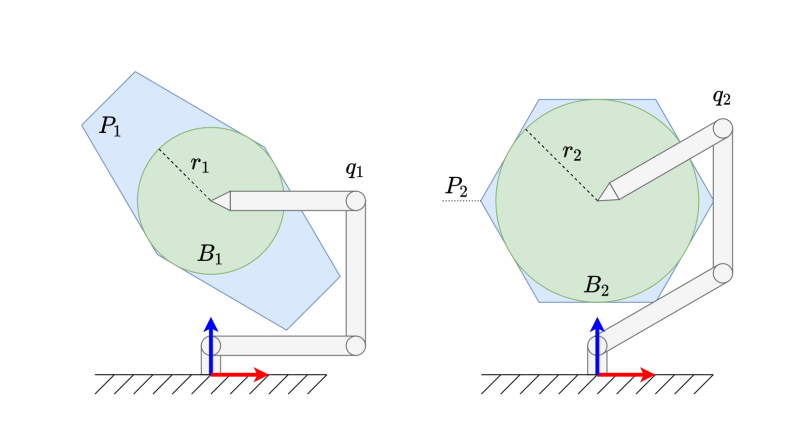
\includegraphics[width=\linewidth]{figures/resdidual_force_polytope}
    \caption{Comparison of two residual force polytopes with identical endeffector position. The blue area represents the maximal forces the system can compensate with the green circle being the worst case scenario. Note that the shapes change with respect to the configuration of the arm.\cite{respoly}}
    \label{fig:resforce}
\end{figure}


\section{Global Robustness in Nonlinear Dynamic Systems} \label{Global Robustness}
It should now become clear that the way robustness is defined and quantified strongly depends on the problem it is applied to. The hurdle in finding a measure for the particular problem at hand is that neither the underlying system nor the applied disturbances are predefined as to preserve generality. 
To find a suitable solution, it is a good idea to formalize the question to a degree. The mathematical representation of mechanical systems is usually given in the form of differential equations $\dot{\textbf{x}} =F(\textbf{x})$, describing the relationship between the states of a system and their change with respect to time. 
Nonlinearities caused by compliance as well as impacts typically occurring in legged locomotion exclude methods applicable to linear systems of equations. 
What remains are nonlinear systems of differential equations which are to be analyzed and ultimately quantified with respect to robustness. 
 
\subsection{Phase Space Representation of Dynamic Systems} \label{Phase Space}
A popular method of visualizing dynamic systems are phase space diagrams, which encompass all possible states of a system. For mechanical systems these states are usually the generalized coordinates and their temporal derivatives, where the dimension of the space scales with the degrees of freedom. Solving the differential equations repeatedly, taking various states as the initial conditions, reveals the global behaviour in the form of trajectories within the phase space. An two dimensional example of this can be seen in Figure~\ref{fig:Limitcycle}.

While the trajectories go on indefinitely, most quickly go to infinity or end up in a cyclic pattern. The latter are called attractors, which are of large interest in the discussion of nonlinear dynamic systems. They represent a set of states which the trajectories will not leave once they encounter them. This might represent the repeating motion of a robotic foot at the end of a leg. An important insight here is that around any attractor there exists a set of states who's trajectories will always converge towards the attractor. This set is called the Basin of Attraction (BoA), however it should be noted that the terms “Domain of Attraction”, “Region of Attraction” as well as “Basin Attraction” are used synonymously in literature.
\begin{figure}[ht]
    %\resizebox{.9\linewidth}{!}{\input{plot.tex}}
    \centering
    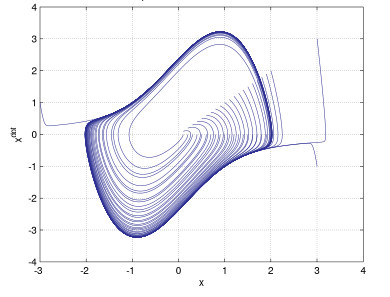
\includegraphics[width=.5\linewidth]{figures/Limitcycle}
    \caption{Phase Space Diagram of a Van der Pol Oscillator. The attractor is indicated by the thick line and the trajectories by thin lines, all converging towards the attractor. \cite{phase}}
    %\scalebox{0.25}{0.25}
    \label{fig:Limitcycle}
\end{figure}

\subsection{Robustness Measures via the Basin of Attraction} \label{Basin of Attraction}

Given that all trajectories starting in the BoA will also always stay within it, a robustness formulation can be derived by taking the effect of disturbances into account. Disturbances generally result in a state changes, which in the context of the phase space corresponds to a jump onto a different trajectory. As long as the new state lies within the BoA, the trajectory will return back to the stable solution and the robot will recover. However if the disturbance is too large, the system will land on a diverging trajectory outside the BoA, quickly leading to failure of the system. To increase robustness, we want to decrease the likelihood of a disturbance moving the system state outside of the basin. Having no control over the types of disturbances that our robot leg might encounter, the geometry of the basin itself needs to be changed. A larger basin will make it more likely that the new trajectory will stay within it, given a random disturbance. The geometry of the BoA is therefore a representation of the system's robustness. To obtain a quantified measure of the robustness, one simple approach is to take the high dimensional volume of the basin.
Rummel et al.\ \cite{walkbasin} have applied this robustness formulation to identify stable walking gaits in a two degree of freedom spring-mass walker model. In this low dimensional case the volume translates to the area of the BoA, which was always bounded for the system analyzed. Of course these basins may take many complicated forms, including fractals and regions that stretch to infinity. Sprott et al.\ \cite{classify} have come up with a method to sort the BoA into classes, listed in Table~\ref{t:class} and shown in part in Figure~\ref{fig:classes}. They achieved this by finding a power law describing the probability of a point laying within the basin, depending on it's distance from the attractor. 

\begin{table}[ht]
\caption[Spacing for units]{\label{t:class}Classes of Basins. \cite{classify}}
\begin{tabular}{l l}
\hline
1       &  globally attracting basins\\
2       &  attracting a fixed fraction of phase space\\
3       & basins extending to $\infty$ in some directions\\
4       & bounded basins\\                
\hline
\end{tabular}

\end{table}
\begin{figure}
    \centering
    \subfloat[\centering Class 3]{{\includegraphics*[width=0.4\linewidth]{figures/IMG_0769.jpg} }}%
    \qquad
    \subfloat[\centering Class 4]{{\includegraphics*[width=0.4\linewidth]{figures/IMG_0770.jpg} }}%
    \caption{Examples of basin classes. The black lines represent the attractors and the blue areas the basins of attraction. Note that in (a) parts of the basin extend to infinity while (b) is bounded. \cite{classify}}%
    \label{fig:classes}%
\end{figure}

Knowing that BoA are not uniform in most cases, the direction of a disturbance within the phase space matters. If the basin border is particularly close to the attractor at any point, the system will be less robust to disturbances in that direction. Comparable to the methodology in Section~\ref{Residual Force Polytopes} Horibe et al.\ \cite{quant} have considering the worst case scenario by finding the shortest distance from the attractor to the boundary of the BoA.
This minimal radius of the BoA is a more conservative measure of robustness. It also allows to disregard complicated parts of the basin that extend to infinity or have strong fractal properties. In \cite{integr} this robustness measure was also determined, however under the name "Integrity Measure".
Coinciding with the goals of this project, \cite{quant} have used this robustness formulation to successfully optimize the physical design of inverted multi link pendulums with respect to control effort.
 
\subsection{Numerical Methods for Basin of Attraction Analysis} \label{Numerical Methods}
In order to quantify the robustness of a system using the BoA, the shape of the basin needs to be explored. Solving the systems of differential equations analytically is often not feasible, requiring numerical methods to be applied. The general procedure is first the sampling of a finite set of initial conditions from the continuous phase space and then integration of the differential equations. One popular method, applied by Brzeski et al.\ \cite{multistable} to quantify the responses of multistable systems, uses Monte Carlo methods for the sampling in which the initial conditions are chosen randomly from a given probability distribution. Finding the corresponding trajectories and determining whether they converge to the attractor gives a picture of the basin geometry. \cite{limitsBoA} explores potential issues with this method and finds that chaotic systems can lead to large cumulative errors in the integration of the trajectories. Furthermore the fraction of space that the basins take up tends to become smaller in higher dimensions, leading to more samples having to be evaluated and in turn increasing the computational cost.
An alternative approach are the “Cell Mapping Methods”, first summarized in \cite{cell1} and recently updated in \cite{cell2} as a comprehensive book. For cell mapping methods, the entire phase space is discretized along each dimension, resulting in a grid of possibly high dimensional, equally sized cells. The center point of each cell is chosen as the initial condition with which the differential equations are solved. The resulting trajectory is computed for a short time period to determine the mapping to a following cell. Repeating this procedure for all cells reveals the global behavior of the system dynamics. The benefit here is that integration errors are only local and stay confined to the basin boundaries. In addition, as the integration of the differential equations is bound to short intervals, each evaluation becomes computationally cheaper.

\begin{figure}[h]
    \caption{One dimensional SCM.\cite{cell1}}
    \centering
    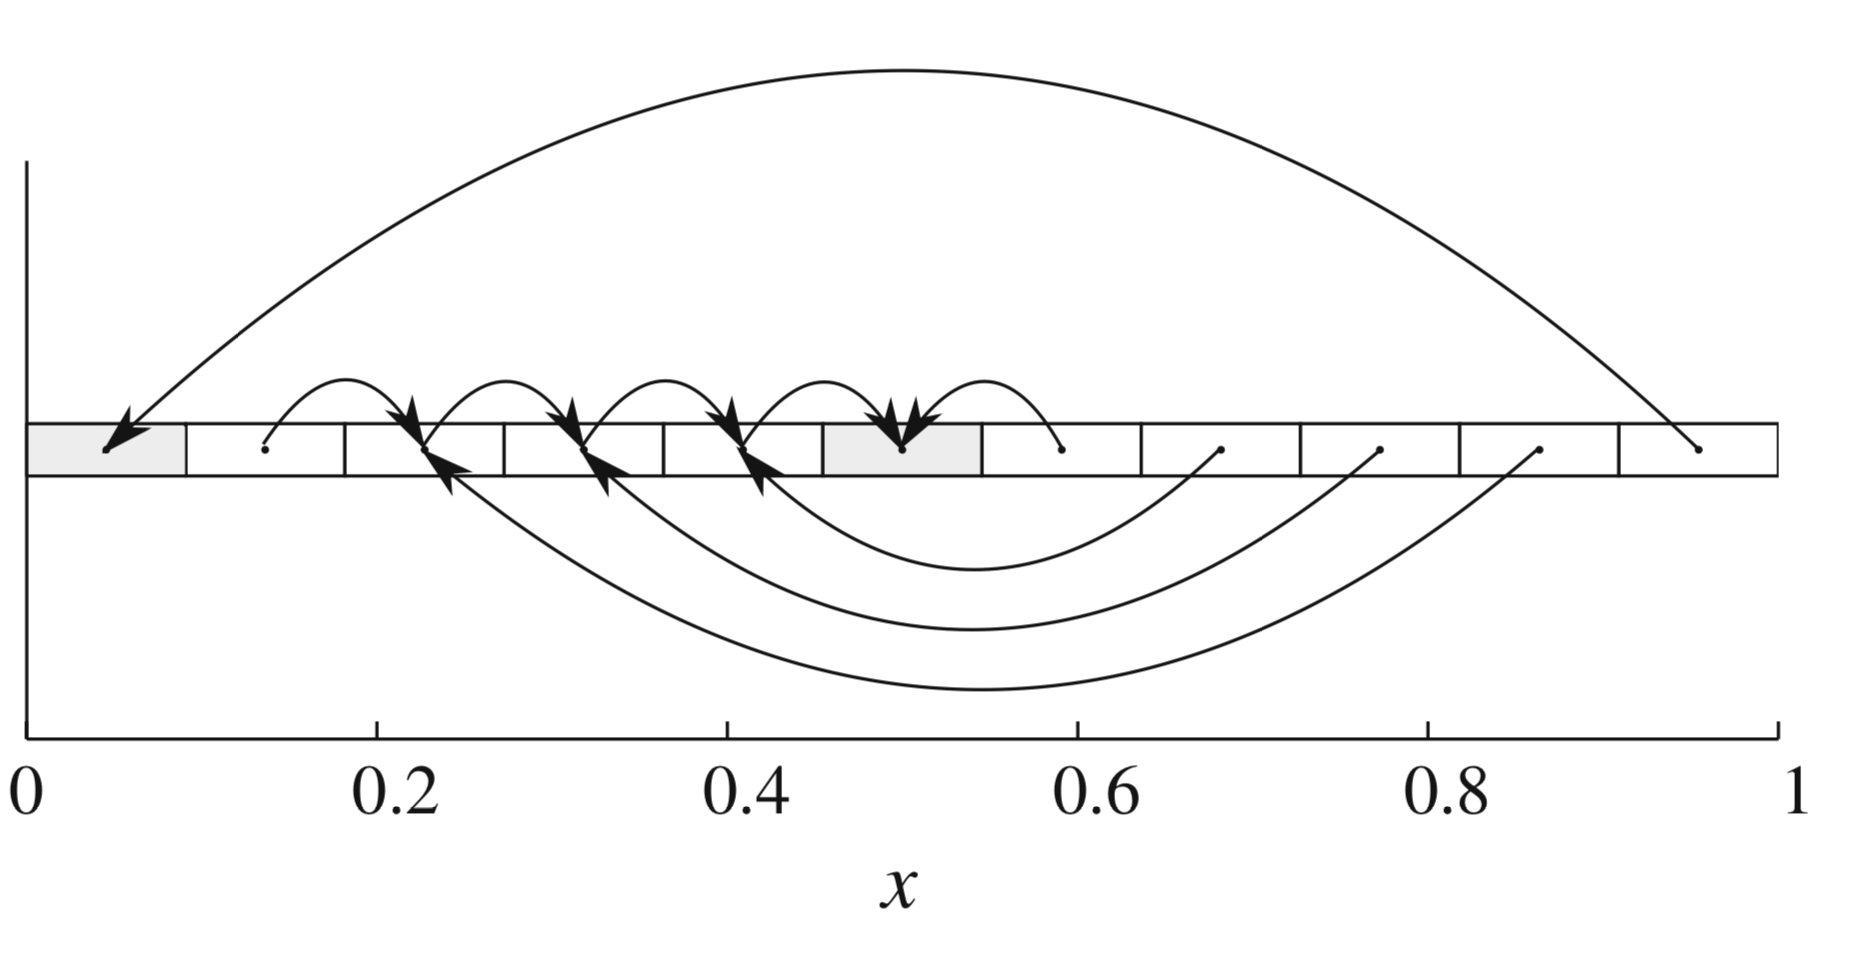
\includegraphics[width=.9\linewidth]{figures/1d-cm}
    \caption{One dimensional SCM. The rightmost cell goes to infinity, which is mapped to the 0 position, the so called sink-cell. With the remaining cells an attractor can be seen at x = 0.5. \cite{cell1}}
    \label{fig:1d-cm}
\end{figure}

This deterministic mapping between cells represents the Simple Cell Mapping (SCM). An issue with it is that it does not consider the infinite amount of initial conditions covered by each cell, which could all potentially result in vastly different trajectories. This discrepancy is overcome with the General Cell Mapping (GCM), a stochastic approach where from each starting cell the probability of landing in any other cell is found. This problem translates to a Markov chain representation, which has been well researched and for which efficient algorithms exist. The GCM is also better at dealing with fractal basin boundaries and can handle chaotic systems. As seen \cite{cell2}, there are many extensions to, as well as hybrids of the SCM and GCM methods, yielding better results. But of course cell mapping methods do have their limitations. 
As always, the curse of dimensionality persists and adding more dimensions exponentially increases the number of cells that have to be evaluated. For the overarching project leg designs with many degrees of freedom need to be analyzed, resulting in high dimensional phase spaces and increasing the computational cost. To overcome this hurdle, there have been efforts in parallelization of the computation by \cite{sixdim},\cite{parallel} and \cite{integr}, allowing for the exploration of higher dimensional systems, with promising results (see Figure~\ref{fig:sboa}). Given the results from any of the Cell Mapping Measures, either the volume or the minimal radius of a BoA can then be found to act as the concrete measure of robustness. 

\begin{figure}[ht]
    \centering
    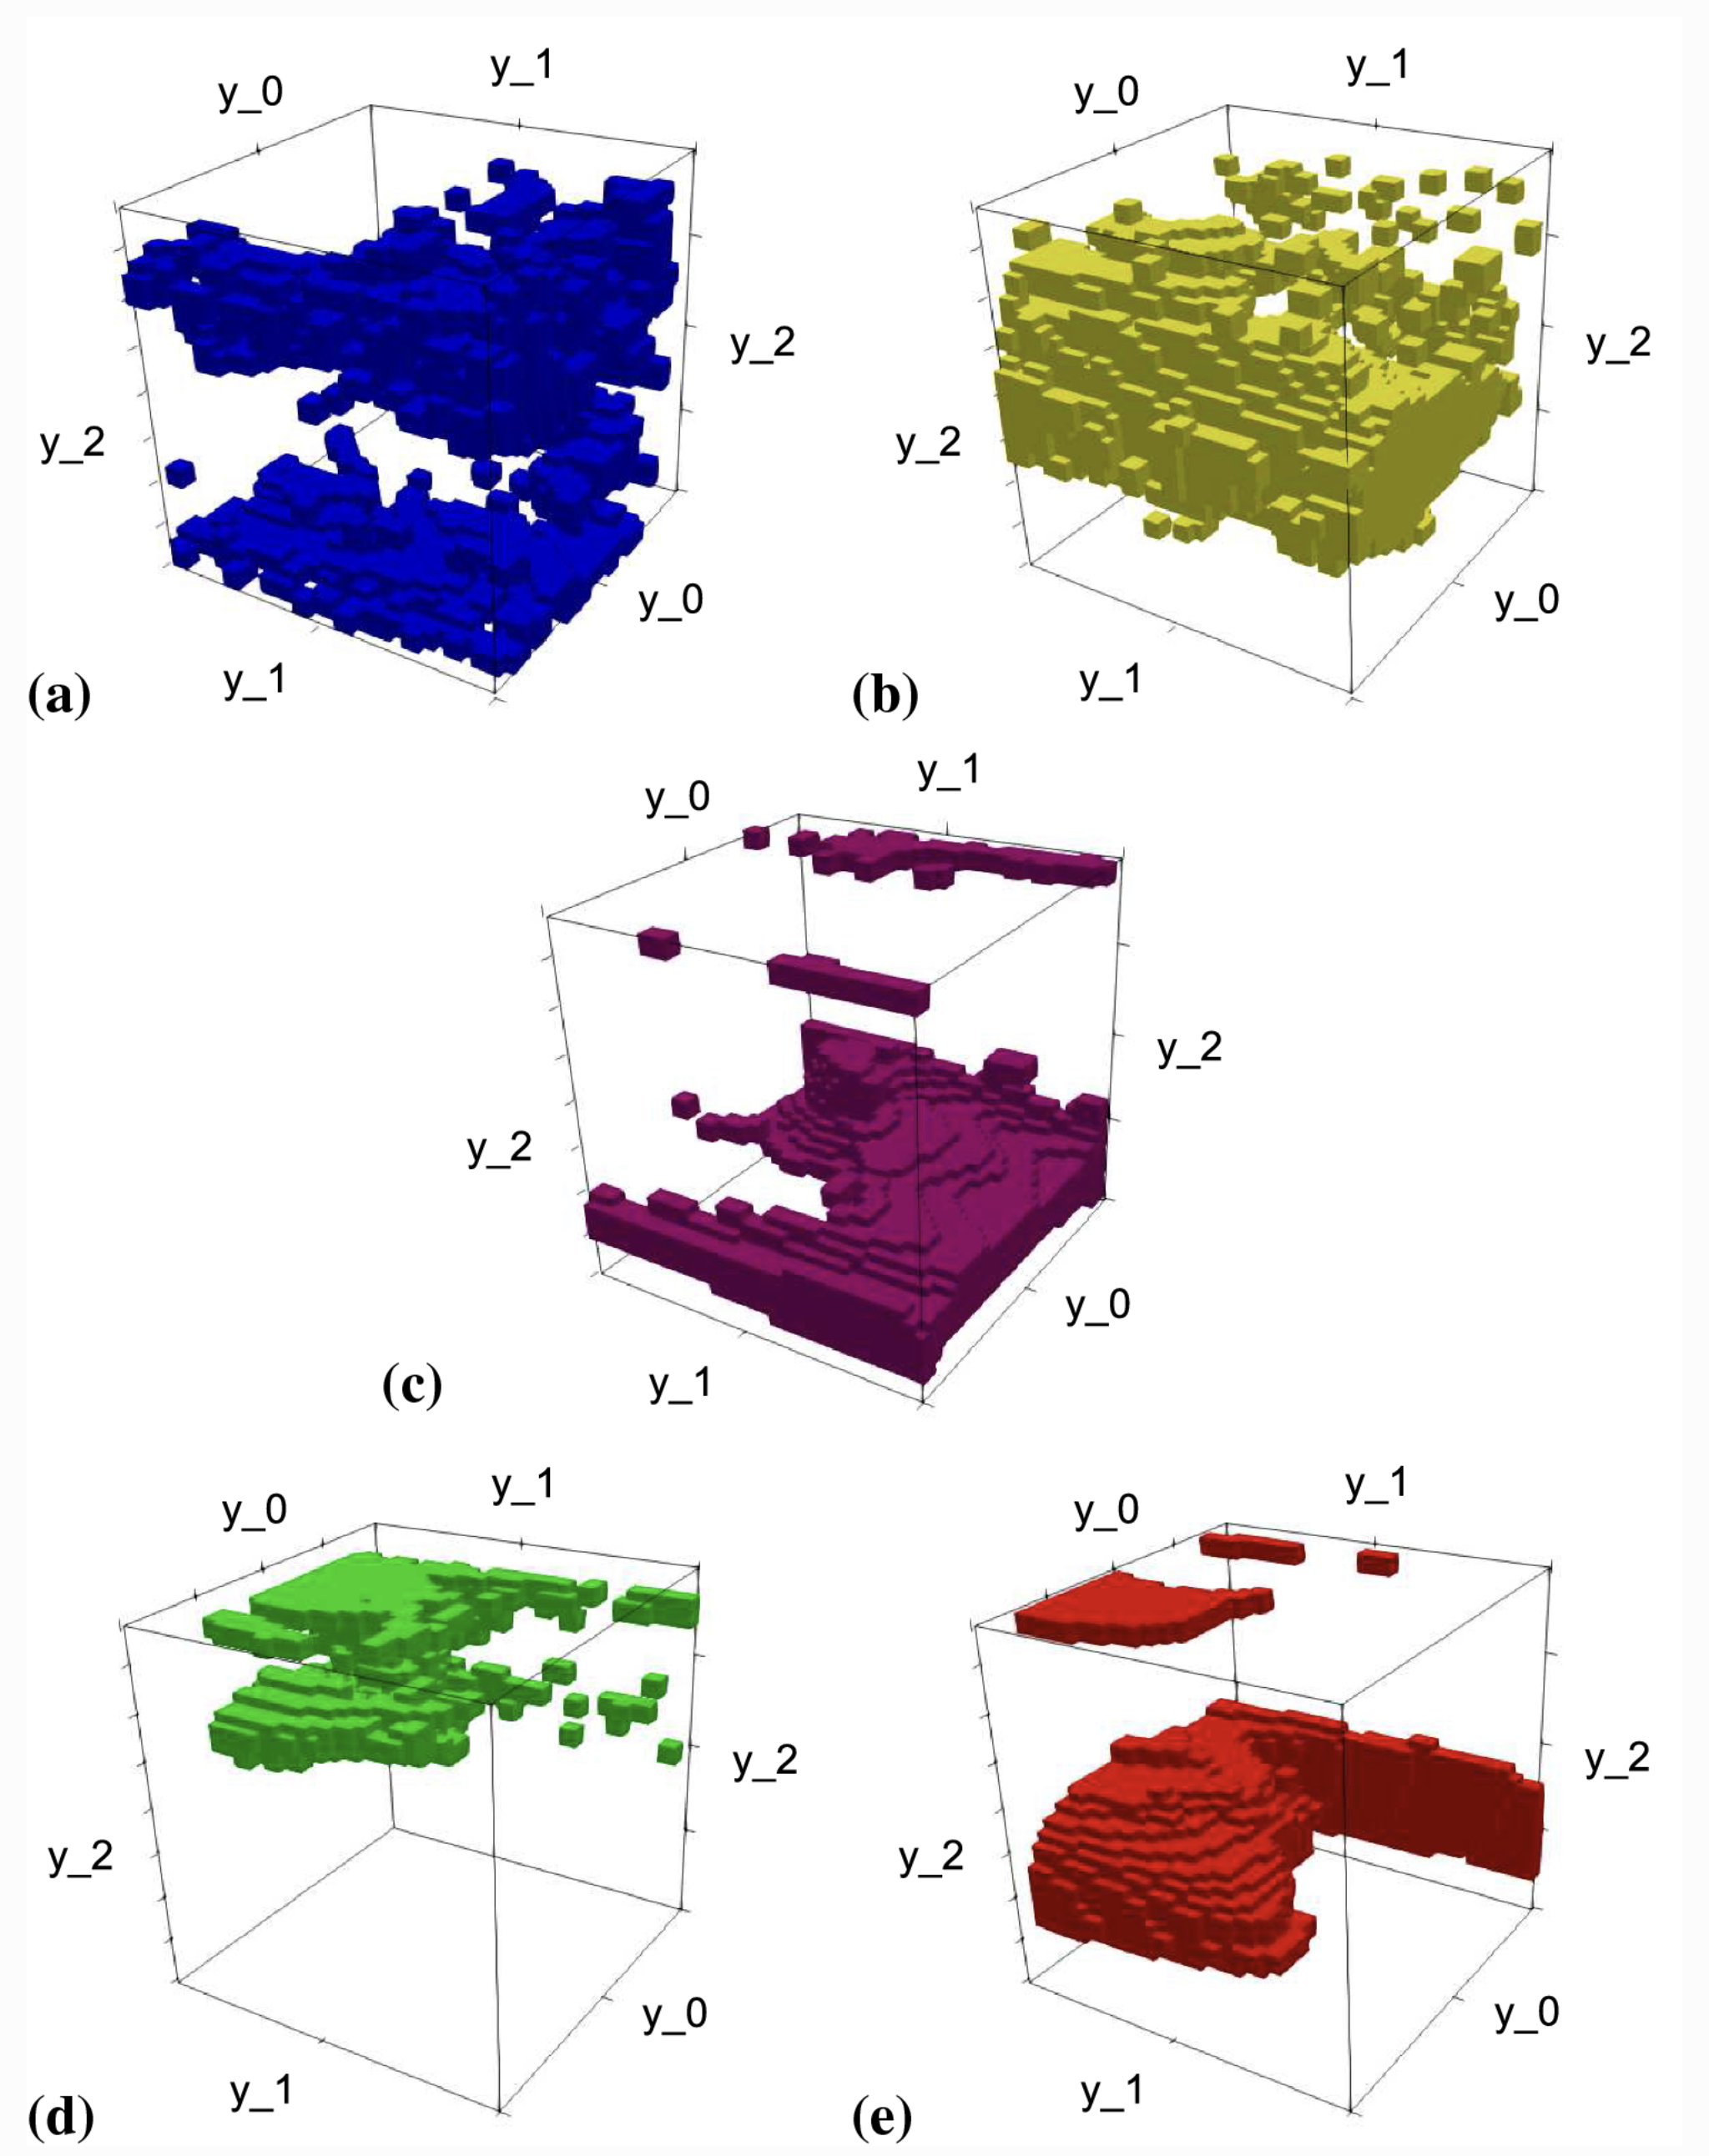
\includegraphics[width=.9\linewidth]{figures/IMG_0783.jpg}
    \caption{3D sections of multiple six dimensional Basins of Attraction. \cite{sixdim}}
    \label{fig:sboa}
\end{figure}


\begin{figure}[h]
    \centering
    %\fontsize{7}{10}\selectfont
    %\includesvg[width=.9\linewidth]{bisection.svg}
    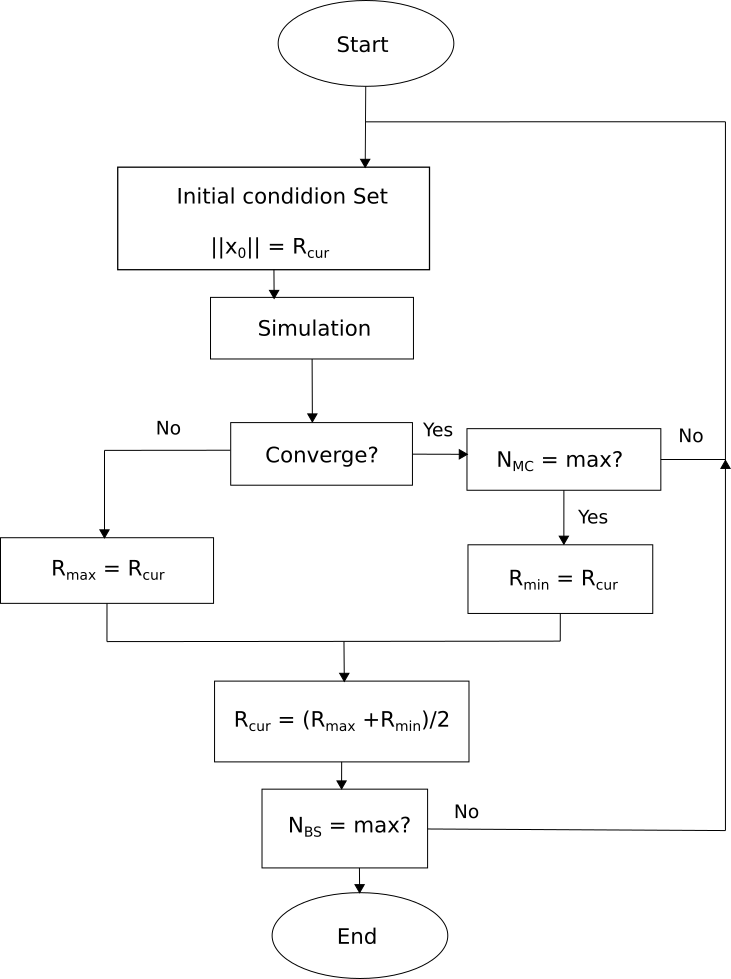
\includegraphics[width=.9\linewidth]{figures/bisection.png}
    \caption{Bisection Algorithm. Using two initial guesses $N_{MC}$ samples at the current radius are evaluated for convergence. If all samples converge the minimal radius is updated, otherwise the maximal radius. This is repeated for $N_{BS}$ iterations. \cite{quant}}
    \label{fig:alg}
\end{figure}

Looking again at \cite{quant}, the robustness was determined without a global exploration, but by strategically sampling initial conditions and using the bisection algorithm to approximate the minimal radius, as seen in Figure~\ref{fig:alg}. For this method the trajectories had to again be evaluated until their convergence could be determined. Still, with the strong reduction of the total number of evaluations to be performed, the computational cost of quantifying the robustness was greatly decreased. 




\newpage
\section{Discussion} \label{Discussion}
The previous sections presented robustness definitions in different fields as well as concrete measures applicable to nonlinear systems. Cell Mapping Methods and random sampling in combination with trajectory evaluation were discussed and their shortcomings as well as their benefits were pointed out. While Cell Mapping Methods have low evaluation costs for each of their cells, the total computational cost rises exponentially when applied to higher dimensions. At the same time they are easily parallelizable, leaving a possibility of reducing the total computational time. The random sampling methods face similar issues in high dimensions with shrinking basin ratios and large errors in the trajectory exploration caused by chaos. Given the geometry of the BoA, the volume of the basin and its minimal radius were presented as specific measures for robustness. The later introduced bisection method presented an improvement on the random sampling approach by determining only the minimal radius of the BoA. An important assumption for this method is the knowledge of the location of the BoA, as the algorithm depends on knowing the distance from the center of attraction. 
The bisection method seems to be the most promising, especially as it has been applied to a problem very similar to the goal of the project. This however also assumes that the input data is a set of differential equations. Given experimental data, it might make sense to incorporate them into the Cell Mapping Methods, possibly mitigating the need for computing the trajectories. In any case, these are all very powerful tools, which can obtain excellent results, given a certain amount of computational resources.
\chapter{Your Central Work}

\section{Theory and Problem Formulation}

    In this section lays out the relvant physical definitions from which the robustness measure is derived and which will be referred to in the later code implementation. all of which are important for understanding and some of which are directly used for the implementation. 

\subsection{Dynamical Systems} \label{dynamicstheory}
    
    Dynamical systems are distinguished by an evolution of their state $\mathbf{x}(t)$ through time. This evolution can be fully described by a set of ordinary differential equations of the form $\dot{\mathbf{x}}(t) = \mathbf{F}(\mathbf{x}(t),t)$, where $\mathbf{F}$ is some nonlinear function. This simplifies to $\dot{\mathbf{x}}(t) = \mathbf{F}(\mathbf{x}(t))$ under the assumption that the dynamical system is autonomous, i.e. is not explicitly dependent on time. 
    When solving for the explicit solution $\mathbf{x}(t)$, an initial condition $\mathbf{x_0}=\mathbf{x}(t_0)$ is required, which is a system state at an initial time. For simplicity and without loss of generality for autonomous systems, one sets $t_0 = 0$. With this the Initial Value Problem (IVP) can be formulated: \begin{gather} \label{eq:1} find \ \ \mathbf{x}(t) \\ s.t. \ \dot{\mathbf{x}}(t) = \mathbf{F}(\mathbf{x}(t)) \\ and \ \ \mathbf{x}(0) = \mathbf{x}_0 \end{gather}
    The solution to the IVP is denoted as $\mathbf{x}(t,\mathbf{x}_0)$. It represents the trajectory of the system state through time given an initial condition. The space in which this trajectory lies is spanned by all possible states $\mathbf{x}$ and termed the $state\ space$. Note that any future state of the trajectoy $\mathbf{x}(\tau,\mathbf{x}_0)$ at time $\tau > 0$ can be taken as an initial condition of the IVP itself. It turns out that the new solution coincides with the initial one, i.e. $\mathbf{x}(t,\mathbf{x}_0) = \mathbf{x}(t,\mathbf{x}(\tau,\mathbf{x}_0))$, which illustrates that any state $\mathbf{x}(t)$ of a trajectory $\mathbf{x}(t,\mathbf{x}_0)$ is suffitient to represent the trajectory as a whole.
    
    Mechanical systems tend to be described in terms of generalized coordinates \begin{gather}\mathbf{q}(t)=\begin{bmatrix}q_1(t)&q_2(t)&\ldots&q_n(t) \end{bmatrix}^\intercal . \end{gather} They are the minimal set of coordinates needed to fully describe the position and orientation of all of the systems elements. Their dimension $n$ cooincides with the number of degrees of freedom of the system. The corresponding differential equations are of second order, depending on $\ddot{\mathbf{q}}(t)$ in addition to $\dot{\mathbf{q}}(t)$ and $\mathbf{q}(t)$. Simply put, this is due to their derivation by Newton's second method, where forces acting on the system are related to the second time derivative via $F = ma$.
    Through an order reduction these differential equations can be cast into the reviously mentioned general form \ref{eq:1}, where \begin{gather*} \mathbf{x}(t) = \begin{bmatrix}\mathbf{q}(t)&\dot{\mathbf{q}}(t)\end{bmatrix}^\intercal .\end{gather*}
    This implies that in order to solve the IVP, initial conditions $\mathbf{q}_0$ and $\dot{\mathbf{q}}_0$ are required. We can also state that for a system with $n$ degrees of freedom (DoF), its state $\mathbf{x}(t) \in \mathbb{R}^{2n}$. The particular state space spanned by generalized coordinates and velocities is termed the $phase\ space$. Within it, states are single points and state trajectories following the IVP are smooth curves. The phase space is used for generalizable qualitative analysis of the behaviour of nonlinear dynamical systems and plays a pivotal role in the fromulation of the robustness measure. It shall be stressed that any instantaneous configuration of the system can be represented as a point in the phase space and it is impossible for the state to exist outside of it. 

    When discussing high level concepts the system state will be refered to as $\mathbf{x}(t)$ for simplicity, while in the code implementation the generalized coordinates $\mathbf{q}(t)$ and velocities $\dot{\mathbf{q}}(t)$ will be more relevant. Keep in mind that both are equivalent.




    %Go over to mechanical systems, explain generalized coordinates and show how this means that the state has q and qdot. Appendix to order reduction. Say how q_0 and qdot_0 are suffitient an necessary to fully characterize the system state. State that the state space for this constellation is called the phase space (used often). Is very interesting for analysis





    %It's elements are coordinates  in a chosen set of coordinates. For convenience we choose the so called generalized coordinates $\mathbf{q}(t)=\begin{bmatrix}q_1(t)&q_2(t)&\ldots&q_n(t) \end{bmatrix}^\intercal$, which describe the system configuration with a minimal amount of coordinates, the number of which coincided with the degrees of freedom of the system. The individual q might represent angles, positions along a specific direction or even along a constrained curve. 

    %to acquire the equations of motion one needs to solve a 2n dimensional system of differential equations of the general form 
    %\begin{align*}
    %\dot{\mathbf{q}}(t) = \mathbf{f}(\mathbf{q}(t),\dot{\mathbf{q}}(t))\\
    %\ddot{\mathbf{q}}(t) = \mathbf{g}(\mathbf{q}(t),\dot{\mathbf{q}}(t))
    %\end{align*}
    %with $\mathbf{f}$ and $\mathbf{g}$ being some general nonlinear functions under the assumtion that the system is autonomous. 
    %q(t) describes the evolution through time.
    %q(t) can only be analytically found in a few cases and quickly breaks down when contact forces and other nonlinearities come into play. 


    %q and qdot are suffitient to describe the system as they are precisely the initial conditions for solving for the trajectory in future time. 


    %This is something for the appendix
    %It is often much simpler to formulate the dynamics in terms of differential equations, which in the case of mechanical systems result in ordinary differential equations with the first and second time derivative of q. 
    


    %$\math

    %The trajectory of a system is the evolution of the state x through time starting from an initial state at an initial time $\mathbf{x}_0 = \mathbf{x}(t_0)$. Explicit for trajectories $\mathbf{x}(t) = \mathbf{F}(t)$ are generally hard to find which is why system dynamics are usually described in the form of an initial value problem using systems of differential equations $\dot{\mathbf{x}}(t) = \mathbf{F}(\mathbf{x}(t),t)$. $\dot{\mathbf{q}}(t) = \begin{bmatrix}\dot{q_1}(t)&\dot{q_2}(t)&\ldots&\dot{q_n}\end{bmatrix}^\intercal$ is denoted as the vector of generalized velocities. 

    %For mechanical systems the 


    %For ease of notation we define the state $\mathbf{x}(t)$ of a system by the concatenation of the generalized coordinates and velocities.

    %$\mathbf{x}(t) = \begin{bmatrix}\mathbf{q}(t)&\dot{\mathbf{q}}(t)\end{bmatrix}^\intercal$



    %the solution of x may depend on anarbitrary order of time derivatives, however it can always be reduced to a first order system of ode's. 

    %we look at dynamical systems of the form of ivps  


    %Here we assume that the differential equations do not explicitly depend on time and are therefore autonomous $\%mathbf{F}(\mathbf{x}(t),t) = \mathbf{F}(\mathbf{x}(t))$.   

    %define state and trajectory first.


\subsection{Attractors and Convergence} \label{attractortheory}
    

    In nonlinear dynamical systems, there may exist sets of states in the phase space which express an attracting behaviour, which means that once a trajectory reaches an element of such a set, all of its future states will also be part of that set. Define an attractor as a set of states:
    \begin{gather} \mathbf{A} \subset phase\ space,\\ s.t.\ if \ \mathbf{x}(t_0) = \mathbf{x}_0\ \in \mathbf{A}, \\ \mathbf{x}(t,\mathbf{x}_0) \in \mathbf{A}\quad \forall\ t > t_0. \label{eq:2} \end{gather}
    Attractors can be divided into two fundamental variants.
    If the attracting set consists of only one state, it is called a fixed point. Fixed points are associated with the condition
    \begin{gather}  \dot{\mathbf{x}}(t) = \mathbf{0}\ \ \forall \ t \in \mathbb{R}, \label{eq:3} \end{gather}
    meaning that the state of the fixed point is unchanging and the related trajectory is reduced to a point. Whether a state $\mathbf{x}(t)$ is a fixed point can be easily determined by checking $\mathbf{F}(\mathbf{x}(t)) = \mathbf{0} \label{eq:4}$. A classical example of a fixed point is the stable bottom position of a pendulum, where if given zero initial velocity, it won't leave the stable position. This is not the case for any other position as gravity will act on the mass (except for the inverted position, however this is practically not realizable), accelerating the pendulum and in turn violating \ref{eq:3}.
    In the general case with $\mathbf{A}$ containing of more than one state, \ref{eq:3} does not hold. Rather the trajectory is moving through the states of $\mathbf{A}$, visiting every each at some point in time and returning to it at future times in a periodic fashion. These types of attractors are called limit cycles. Finding them is generally a hard problem, but for simpler cases one can check:
    \begin{gather} If\ for \ \mathbf{x}(t,\mathbf{x}_0) ,\ t > 0 \quad \exists \quad \mathbf{x}(\tau) = \mathbf{x}(\tau + h),\ \tau > 0,\ h > 0, \\then\ \{\ \mathbf{x}(t) \mid t \in [\tau,\tau + h)\ \}, \ is \ a\ \mathbf{limit\ cycle}.\label{eq:5} \end{gather}
    An example for this case are the compliant linkages described in (REF: strandbeest compliant version), where the end effector follows a cyclic trajectory in its undisturbed state. 
    In section \ref{codeimplementation}, methods for dealing with both types of attractors and the problem of applying the continuous analysis in a discrete setting are provided. 

    For any initial condition not part of the attractor, the related trajectory may land and stay on the attractor after some time $t > t_0$. 
    \begin{gather} \label{eq:6} Given\ an\ attractor\ \mathbf{A},\ for\ any\ \mathbf{x}_0 \notin \mathbf{A}\\ if\ \ \underset{t \rightarrow \infty}{lim} \ \mathbf{x}(t,\mathbf{x}_0) \in \mathbf{A}\ \Rightarrow\
    \mathbf{x}(t,\mathbf{x}_0)\ \mathbf{converges}\ to\ \mathbf{A}\ \end{gather}
    Should the definition above not hold, the trajectoy is denoted as diverging (as in cell mapping methods). 

    Note that there may exist any number of attractors in the phase space of a system (REF: paper with multitude of attractors). Convergence is always defined with respect to a particular attractor $\mathbf{A}$, which needs to be specified. Therefore if the trajectory converges to a different attractor, it is still defined as diverging from the attractor of interest.  

    The set of all states for which the resulting trajectories converge to the attractor of interest is called the $Basin\ of\ Attraction$ (BoA) and is defined as: 
    \begin{gather} \label{eq:7} BoA = \{\ \mathbf{x}_0 \in \mathbb{R}^{2n} \mid  \underset{t \rightarrow \infty}{lim} \ \mathbf{x}(t,\mathbf{x}_0) \in \mathbf{A}\ \}\end{gather}
    where $\mathbf{A}$ is an attractor as defined in \ref{eq:3}.

    From here on the general attractor of interest is represented by $\mathbf{A}$.
    Additionally, disturbances are defined as any event that acts upon the system, inducing a state change. This new state implies a new trajectory as a solution of the IVP, resulting in future system behaviour that may differ vastly from the undisturbed case.




    %Formally, a trajectory converges to an attractor A iff $\underset{t \rightarrow \infty}{lim}\mathbf{x}(t) \in A$
    %We denote an initial condition which ends up at the attractor of choice as converging towards the attractor. Any initial condition for which this is not true is said to diverge. Note that there may exist any number of attractors in the phase space (reference paper with multitude of attractors) towards the  which is why a particular attractor needs to be specified. If the attractor converges a different attractor, it is still defined as diverging from the attractor of interest.  
    %The attractor of interest is can be found by simulation, but often it already clear a priori, mostly in the form of the undisturbed state. 

    %Within bounded time intervals, the evolution of a state trajectory can be described by two main behaviours. Either it stays confined to a set of states   (also reference cell mapping algorithms which do exactly that).


    %The phase space is a particular instance of state spaces, restricted to the set of generalized coordinates $q_i$ and their corresponding generalized velocities $\dot{q_i}$, sometimes in form of generalized momenta (via scaling by mass or inertia). It encompasses all possible initial conditions of a mechanical system and solutions of of the ivp result in trajectories through the phase space, starting at 


    %Starting with a system and an initial condition that is part of an attractor 

   % Attractors are sets of states in the phase space
    %In a general nonlinear dynamical system, the evolution of the state can be divided into two main events using the concept of attractors. Attractors are sets of states toward which the system trajectories will converge or diverge from. If the set only consists of one state it is called a fixed point, else a periodic orbit where the trajectory will visit all states of the set periodically if given enough time. 
     
    %The set of initial conditions in the phase space for which the resulting trajectories converge towards the attractor is called the basin of attraction. If an initial condition does not lie in this set, it's trajectory diverges from the attractor. 
     

    

    

\subsection{Robustness Measure} \label{robustnessmeasure}

    The robustness measure proposed in REF and implemented in the following is derived using the concepts of nonlinear dynamics outlined in the previous section. In order to improve feasibility when applied to high degree of freedom systems, a slight reframing of the theroy and implementation is proposed.
    
    %INTERPRETATION OF CONVERGENCE
     %Disturbances in mechanical systems can generally be viewed as external forces acting on the system. 
    Given a dynamical system, assume that it holds a desired pose or behaves in a periodic fashion in its undisturbed state. We can interpret these types of behaviour as attractors in the phase space of the system. Applying disturbances will change the system state in ways that are hard to predict as the IVP doesn't hold while the disturbance is acting. In the instant the disturbance stops however, the state $\mathbf{x_d}$ can be used to compute a new trajectory in accordance with the IVP. With this one can evaluate whether the disturbed trajectory converges back to the attractor or fails to do so, implying divergence. %Disturbances resulting in disturbed states lying on the attractor or within the BoA will trivially lead to recoveries, while any state outside of these sets will cause a fatality. 

    \begin{figure}
    \centering
    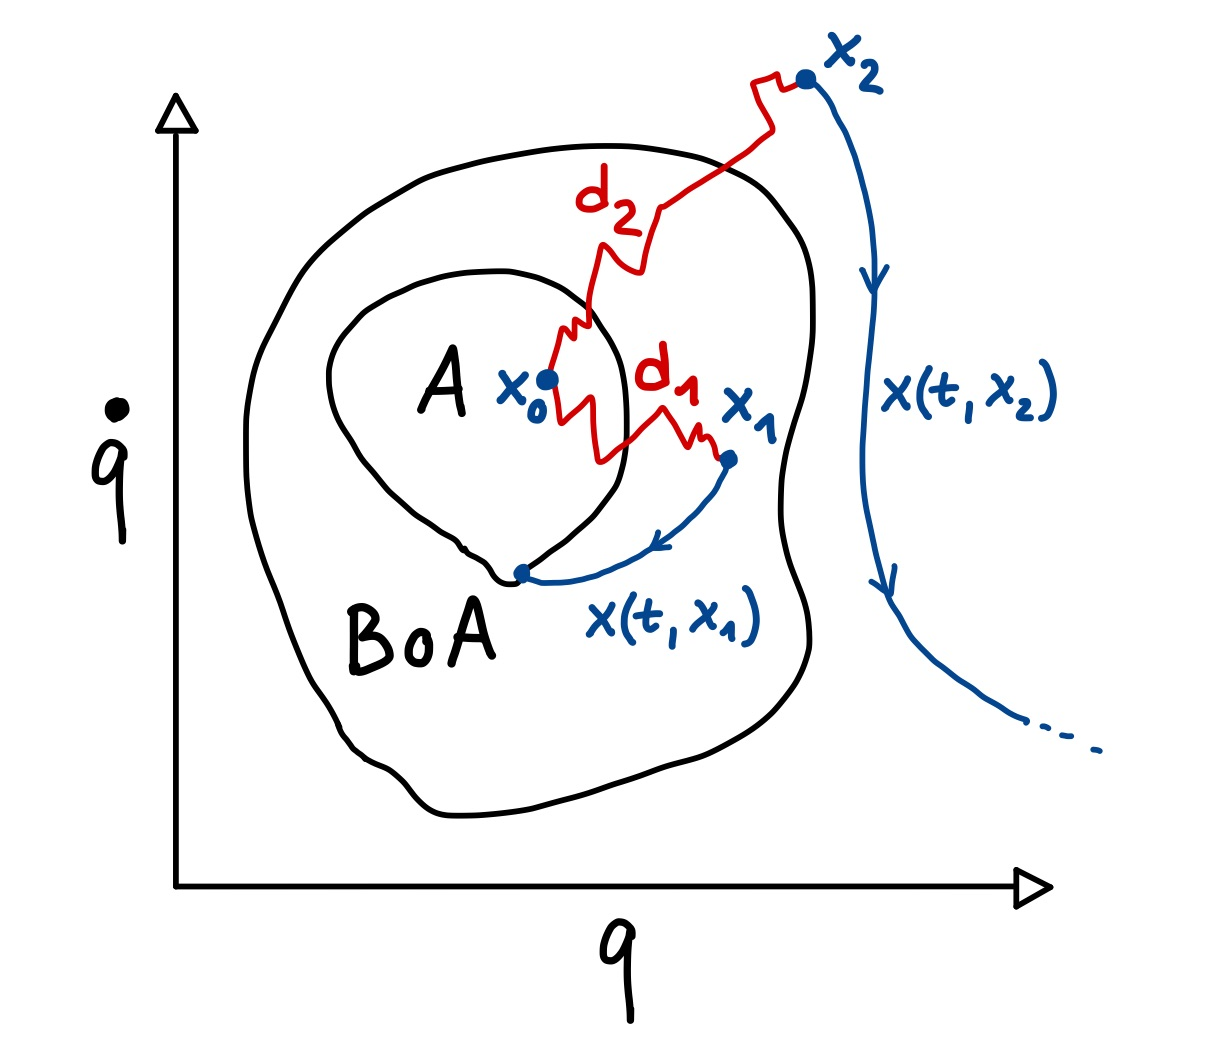
\includegraphics[width=.5\textwidth]{figures/conv_div_viz_crop.png}
    \caption[Convergence and Divergence in the Phase Space]{Effect of differnt disturbances in the phase space. Both trajectories start with a state $\mathbf{x}_0$ on the attractor which is disturbed by two different disturbances $d_i$. $d_1$ results in a disturbed state $\mathbf{x}_1$ in the BoA, the trajectory of which by definition converges back to the attractor. $d_2$ results in a disturbed state $\mathbf{x}_2$ outside the BoA and hence diverges. The IVP holds on the blue parts of the trajectory only.}
    \label{convdiv}
    \end{figure}

    Because of the direct relation between disturbances and state changes, one may choose to analyze only the convergence behaviour of states in phase space. This is how the robustness measure was formulated in REF. The size of the set of states in the phase space resulting in convergence is the measure for robustness. Notice that this is precisely the basin of attraction as defined in \ref{eq:7}. As outlined in REF, finding the size of the BoA is nontrivial, for which the conservative measure of the minimal radius as the shortest distance from the origin to the boundary of the BoA was introduced. One may also think of this as the radius of the largest hypersphere that is still fully contained within the BoA.

    While this measure is rather straight forward to implement, it becomes quite computationally expensive for systems with high number of DoF. 
    In the paper the computational time for a system with just two DoF was already 15 hours for a total of 225 robustness measure computations. The most complex system analyzed had only six DOFs. For comparison, the quadruped model to be analyzed here has 78 DoFs. The exact dependency of the computational effort on the DoF's of the system is hard to determine because of the stochastic nature of the process (see section \ref{minrad}). However in the 6 DoF test in REF, evolutionary algorithms had to be applied as computation of a discretized phase space was no longer feasible, implying that upscaling will be very compuationally expensive. One may choose to measure robustness taking only some dimensions of the phase space into consideration, however in this case the robustness measure is valid only for that subset of the system. This makes its applications less useful, as one would only measure the robustness of a single leg for example, which does not guarantee implications for the whole system. Clearly, some other method of sampling the disturbances is needed.

    Recall that the disturbed states sampled in the phase space are results of underlying disturbances. Given a dynamics engine capable of simulating the disturbances in addition to the system itself, one can compute the complete disturbed trajectories, starting from a state on the attractor. This enables direct application of arbitrarily chosen sets of disturbances to the system, removing the requirement of needing to sample full states. Here a $d$-dimensional disturbance space $\mathsf{D}$ is defined, from which disturbances $\mathbf{s}_{\mathsf{D}}$ will be sampled and in which robustness will be measured. The idea is to transfer the concept of the minimal radius to this new space to approximate the size of the set of disturbances the system will recover from. Note that convergence of the system under a disturbance will still be evaluated by verifying convergence of the state trajectory to the attractor in the phase space. This choice however rules out the application of the cell mapping methods presented in \ref{Numerical Methods}. 

    Denoting $\mathbf{x}(t,\mathbf{x}_0,\mathbf{s}_{\mathsf{D}},\mathbf{s}_{\mathsf{P}})$ as a trajectory that is disturbed at least once for $t > 0$ and given some $\mathbf{A}$, the robustness measure
    \begin{gather} \label{eq:8}
        %robustness\ measure = \min \norm{ s_{\mathsf{D},rec} }\, \{s_{\mathsf{D},rec} = \mathbf{s}_{\mathsf{D}} \in \mathsf{D} \mid \underset{t \rightarrow \infty}{lim} \ \mathbf{x}(t,\mathbf{x}_0,\mathbf{s}_{\mathsf{D}}) \in \mathbf{A}\ \}\\
        %robustness\ measure = \min_{s \in \mathsf{D}_{f}} \norm{ s }\ ,\ \mathsf{D}_{f} = \{\mathbf{s}_{\mathsf{D}} \in \mathsf{D} \mid \underset{t \rightarrow \infty}{lim} \ \mathbf{x}(t,\mathbf{x}_0,\mathbf{s}_{\mathsf{D}}) \notin \mathbf{A}\ \forall\ t > 0 \} \subset \mathsf{D}\\
        RM = \max r\ \in \mathbb{R}^+ \ \ s.t.\ \forall\ \mathbf{s}_{\mathsf{D},r} \in \{\mathbf{s}_{\mathsf{D}} \in \mathsf{D} \mid\ \ \norm{\mathbf{s}_{\mathsf{D}}} = r\}:\ \ \underset{t \rightarrow \infty}{lim} \ \mathbf{x}(t,\mathbf{x}_0,\mathbf{s}_{\mathsf{D},r},\mathbf{s}_{\mathsf{P}}) \in \mathbf{A},\
        %\mathsf{D}_{f} = \{\mathbf{s}_{\mathsf{D}} \in \mathsf{D} \mid \underset{t \rightarrow \infty}{lim} \ \mathbf{x}(t,\mathbf{x}_0,\mathbf{s}_{\mathsf{D}}) \notin \mathbf{A}\ \forall t > 0 \} \subset \mathsf{D}
        %robustness measure is the smalles (norm) of any element of the set of disturbances for which the state trajectory converges to the attractor.  
    \end{gather}
    is defined, where $\mathbf{s}_{\mathsf{P}}$ denotes a set of constant system parameters.
    In other words, RM is the largest radius $r$ for which all disturbances sampled at that distance from the origin will lead to convergence of the disturbed state trajectory.

    %s_{\mathsf{D},rec} = \mid \mathbf{s}_{\mathsf{D}} \in \mathsf{D}




    %Given a solver that can simulate the disturbances as well, trajectories can be computed even while outside forces are acting on the system. This opens the possibility to directly sample and apply disturbances to the system and evaluating the full disturbed trajectory for convergence to the attractor.

    %Examples of this might be holding a specific pose or walking with a periodic gait.

     %Following the new trajectory, one can detemine whether the system will converge back to the attractor. In such a case successful recovery of the system from the disturbance is achieved; one might say the system is robust to that disturbance. %If the following trajectory converges back to the attractor this implies that the system recoveres successfully from the specific disturbance applied to it. 

    

    %Note (add into previous paragraph, that disturbances can do "anything" to the trajectory, i.e. mustn't be continuous, etc. But once the disturbance stops, we can take the state that the system is in at that time to compute the future dynamics, given that no more disturbances are applied. Else we repeat until no further disturbances.)



    




    %Note that a this holds for multiple consecutive or distributed disturbances as well, as only eventual convergence of the trajectory is relevant. Here the IVP has to be solved repeatedly after every new disturbance. %If successful recovery does not occur, it is a failed recovery. 

    %NOTION OF ROBUSTNESS
    %One might also say that the system is robust with respect to that type of disturbance.

    %I want to first explain the REF approach FULLY. 


    %Using these binary responses and under the assumtion that disturbances occur isolated, we can formulate a measure of robustness as in REF.

    %For a robust system, we expect it to recover from more disturbances than one that is not. 
    %(Analyzing all the states in the phase space corresponds to analyzing the effects of any type of disturbance, for times after the end of the disturbance)
     %(quickly describe the minimal Radius here, also do a mathematical formulation).

    %for these types of disturbances it suffices to analyze the convergence of states without regarding the specific disturbance that caused them. The set of converging 


    %We expect a system we denote as robust to recover from more disturbances than one that is not. 


    %Illustrate issue of full state space by introducing Laikago. 78 DOF => 156 dimensional phase space. Applying frameowork on full state space is infeasible. Using just a few dimensions is often not realistic to occur in the real world (just one leg or even joint being disturbed). Therefore we need a way to find a subset of the phase space that can be derived from real world disturbances. 
    %Here we take into account . 
    %We do not sample single states, but apply disturbances directly to the model in the simulation. By this we acquire nontrivial disturbed states that can be described via simple disturbances. The evaluation of convergence stays exactly the same as before. 

    %While this approach has a strong foundation in nonlinear dynamics theory, it quickly becomes infeasible for more complex applications. In the paper the most complex system had six DOFs and the computational time was already high (numbers??). 
    %The system on which most of the test were executed is a simple model of a quadruped which aready has 78 degrees of freedom implying a 156 dimensional phase space. If one for example wanted to discretize the space with just 3 nodes along each dimension, $2.697x10^74$ initial conditions would need to be evaluated. We clearly need to restrict ourselves to a subset of the phase space. One approach would be choosing only small number of dimensions of the phase space, however then the robustness measure is valid only for a part of the system, making it applications less useful, as one could only look at the robustness of a single leg for example. (too long)

    %(The thing is, we don't actually want to discretize the phase space. That's why we use the minimal Radius in the first place. Rather we need to achieve a certain sample density on the surface of the hypersphere defined by the minimal radius in order for the minRad algorithm to work properly. As the surface of a n-dim hypersphere actually becomes quite small for very high dof, this should actually not be an issue... What is an issue, however is that the scaling of all of the different coorinates $q_i$ matters. Findin a scaling such that relevant disturbances have more of an effect on the robustness measure seems quite tough. It would be better to restrict the choice of disturbances/I.C. derived from disturbances. 
    %One argument from a practical perspective is that one needs to verify the results from the minRad algorithm somehow (we did that! overlay!) this becomes tough for any $\mathsf{D}$ with $dim(\mathsf{D}) > 2$ already, as visualization becomes difficult, but then we can point to the issue of subspaces of the phase space only having limited meaning, i.e. robustness of only a small part of the system 

    %A different way of choosing a subset of disturbances is needed. 
    

    %"find the minimal distance to boundary of converging set, where converging set is all elements of DS, for which trajectory will go to attractor in limit within the phase space"
    
    %The goal of finding a robustness measure can be though of as $RM:\mathbb{R}^p \rightarrow \mathbb{R}$, i.e. a mapping from the p-dimensional parameter space to a scalar value.
    %(maybe this goes into the next section)
    

    %Then state why we need to change it (only single intantantaneous forces considered, cannot test specific types of disturbances. phase space becomes veeery large in high dof systems) 

    %(also why it's better)

    %Then we explain how we sample from the DS (after defining it, 0 disturbance at origin, etc) using the same method

    


    

    %REF APPROACH AND APPLICATION TO OUR CASE
    %DESCRIPTION OF HOW ROBUSTNESS IS DEFINED
    %A solution to this can be taken from REF, which used the the same underlying concept for their robustness formulation, just that disturbances arr not explicitly specified. Instead, only the resulting disturbed states are analyzed to determine a measure of robustness which has a more global nature (rephrase). 




    %DESCRIPTION OF HOW TO ACTUALLY GO ABOUT MEASURING
    %While there exist a fair bit of analysis on BoA's their highly complex shapes makes precisely determining their size quite difficult. The approach to overcome this issue is the fromulation of the minimal Radius of the BoA as a conservative measure, restated in the following:

    %It describes the shortest distance from the origin to the boundary of the BoA which can be found using iterative aproaches, detailed in section (minRad). 

    %ADAPTATIONS / REDEFINITION

    %We transfer the concept of the minimal Radius to the Disturbance Space (DS), where the origin represents zero disturbances and each dimension represents the magnitude of a single component of the full disturbance applied. (add mathematical def of DS)
    %With that we can analogously measure robustness by finding the minimal radius of the set of disurbances in the DS, for which the state trajectories in the phase space converge to the attractor.
    %(formally define minimal radius wrt DS)

    %In other words, any combination of disturbances which lies on the surface of the hypersphere with the minimal radius in the DS will result in a trajectory that converges to the attractor in the phase space. 

    %To summerize, while ref was maximizing the number of states resulting of unspecified disturbances, for which the related trajectories converge to the attractor, we are trying to maximize the number of disturbances, for which 

    %When when optimizing for robustness we want to maximise the set of disturbances, which we can do by changing the system paramterers. 
    %IMPLICATIONS OF ADAPTATIONS

    

    %While we still determine convergence by checking the state trajectory wrt the attractor in the phase space, disturbances will be sampled in the DS, meaning the minimal radius also lies in the disturbance space. Nice thing is that any disturbance one can come up with can be tested, but generalizbility to other disturbances (for which one doesn't evaluate the robustness) ceases to exist (rephrase)

    


    %We sample in the bounded DS, evaluate convergence of disturbed system via convergence to the specified attractor in the phase space and 
    

    %Taking sampling initial conditions form the phase space as disturbances gives a nice physical interpretation and in "REF" this was denoted as general robustness (or was it?), however as a counterexample, periodic or constant disturbances are cleary not covered by this. 
    %This is why we worked with general disturbance spaces that can be chosen to work for the particular application at hand. 
    %Note that the trajectory will still lie in the phase space and convergence evaluation 


    %Describe robustness measure from paper but for the actual definition use the general disturbance space. 


\subsection{ Parameter space and Disturbance space}
    
    In order to apply the concept of the minimal radius as a measure of robustness in the disturbance space $\mathsf{D}$, one must impose some conditions on it.
    In the phase space, the origin is generally chosen such that the attractor of interest lies on or in close viscinity to it. This means sampled points $\mathbf{s}_{\mathsf{D}} \in \mathsf{D}$ with a small norm represent no or very small disturbances, guaranteeing convergence of the state trajectory if $\norm{\mathbf{s}_{\mathsf{D}}}$ is chosen small enough. The minimal Radius approach builds on the fact that the origin lies within the converging set and the it's boundary is reached at some point when moving farther away. 
    For this reason me must ensure that in $\mathsf{D}$ the origin also represents the state being on the attractor, implying no disturbance.
    Each element of the disturbance space is just a vector of coordinates representing a single or multiple disturbances. To impose the above condition it must be ensured that the 0 vector in $\mathsf{D}$ represents no disturbance. 
    Taking oscillations as an example one might want to represent them in a 2 dimensional DS with amplitude and frequency as the coordinates. An oscillation with either 0 amplitude or 0 frequency implies no oscillation at all, making this choice valid.
    An invalid example of a coordinate is the direction of a force applied. If the angle of attack is 0, the disturbance itself is clearly non zero, breaking our condition.
    Here, given an initial condition $\mathbf{x}_0$, the $set\ of\ convergence$ 
    \begin{gather} \label{eq:9}
    \mathsf{D}_c = \{ \mathbf{s}_{\mathsf{D}} \in \mathsf{D} \mid\ \underset{t \rightarrow \infty}{lim} \ \mathbf{x}(t,\mathbf{x}_0,\mathbf{s}_{\mathsf{D}},\mathbf{s}_{\mathsf{P}}) \in \mathbf{A}\ \}\end{gather}
    is defined to be quantified by the minimal radius as the equivalent to the BoA.
    For any set of valid coordinates, their scaling w.r.t. each other turns out to considerably affect the resulting robustness measure. Just choosing different units for any coordinate will stretch $\mathsf{D}$ along the corresponding dimension, changing the shape of the converging set and in turn changing the minimal radius to its boundary. This issue is alluded to in the paper REF by allowing the minimal radius to trace an elliptical shape, which corresponds to rescaling one dimension. There seems to be no comprehensive solution to this issue, which is why finding a well posed $\mathsf{D}$ by trial and error is crucial. 
    Conversely, this problem may also be leveraged for controlling later optimization of robustness. If the boundary of the converging set is a given distance away along a dimensions, shrinking that dimension will move that boundary closer to the origin, making it more likely that the minimal Radius lies in that direction. With this the scaling of the coordinates could be seen as a weighting of how important robustness against that part of the disturbance is. 


    For the aforementioned optimization, the parameter space $\mathsf{P}$ is defined to perform the optimization in. Each element $\mathbf{s}_{\mathsf{P}}$ of $\mathsf{P}$ is a set of parameters describing some parts of the underlying system. A different set of parameters will fundamentally change the system and for each element of $\mathsf{P}$, robustness can be evaluated. Eventually the vector of parameters for which robustness is maximized is to be found:

    \begin{gather}\label{eq:10} \max \text{RM}(\mathbf{s}_{\mathsf{P}}),\ \mathbf{s}_{\mathsf{P}}  \in \mathsf{P}\end{gather}

    Methods on finding the optimal set of parameters $\mathbf{s}_{\mathsf{P},opt}$ are presented in section \ref{opt}.
    %sNote that the choice of $\mathsf{P}$ is fundamental for the results. 




    %The choice of parameter spaces (have I mentioned them before?) and disturbance spaces
    %I feel like this should be part of the robustness measure

    %separate from "dynamics", focus on 

    %dimension disturbance space equals d

    %We define the $Disturbance\ Space$ (DS) as the d dimensional space in from which we sample the disturbances. As in REF, 
    %The disturbance space is defined as the set containing all combinations of disturbances, against which the robustness of the system is evaluated. The choice of disturbances in "REFERENCE" are the initial conditions in the phase space (reference to the section in related work or copy that here) as they can be interpreted as the direct result of external forces. In general however, the disturbances may be chosen arbitrarily and the resulting robustness measure will quantify robustness against these. Examples of this were initial tilting of a quadruped over pitch and roll axes and oscillations with the disturbance space spanning the amplitudes and frequencies. Tuple combinations are favoured in testing because of their ease of visualization and mild computational power requirements.  

    %"REFERENCE" chose the DS to coincide with the phase space, as elements of it can be directly interpreted as the result of external forces on the system. This choice is not always feasible nor necessary, as will be shown in the following sections. 

    %It may coincide with the phase space as implemented in "REFERENCE", in which case disturbances can be interpreted as the effects of external forces acting on the system. This moves the system onto a different trajectory 
    %, however it will be shown in the following sections, that this is not always feasible nor necesseary. Especially in systems with a large number of degrees of freedom n, the resulting disturbance space is 2n dimensional. 

    %case DS = phase space: d

    %dimension parameter space = p
    %The two main variable spaces of relevance move are the parameter space (PS), where each dimension represents the value of a chosen system parameter. T (really it also depends on the disturbance space) Finding the best system parameters with respect to the resulting robustness can be formulated as an optimization problem ...


    
    %state space v phase space


\section{Code Implementation} \label{codeimplementation}

This section details the implementation of the robustness measure and its optimization. 

\subsection{Framework Overview} \label{framework}

The framework for the computations seen in figure \ref{fig:framework} was written in c++ while visualizations were created in Python.  

It begins by initializing the simulation, in particular setting the current system parameters. For this adapted system, the corresponding attractor is computed, which it will differ for systems with different parameters. With this and given an initial guess for the upper bound of the minimal radius, the minRad algorithm starts. It repeatedly samples disturbances, applies them to the system and evaluates the disturbed trajectories in order to iteratively update its guess, approaching the true minimal radius. Once a predefined number of iterations is completed, the final guess is taken as the robustness measure for the particular set of system parameters. For the optimization, the robustness measure is used to update the guess of the optimizer, which then samples new sets of parameters, beginning the cycle anew. 


The implementation was built up such that for a different system, only two functions need to be adapted, namely the one handling the setting of new parameters and the one 
in charge of running the simulation and evaluating convergence. Examples of this can be found in section \ref{app}.


%First iterations of the implementation were naively done in a "top down" fashion that was specific to a particular system. This ledLater this was changed such that the relevant (and changing) functions were isolated and could quickly be redefined for new applications. 
%differential equations are implicitly represented as simulation objects in dde. Their parameters can be set. The state x as well. Use the solver to compute the trajectory under a disturbance for a given amount of timesteps. check if trajectory converges or diverges. Do this repeatedly with initial conditions sample
%talk about how knowing the exact shape of the basin of attraction is not necessary for optimization of the robustness, with this and because of the additional work needed to implement the cell mapping algorithms, the method with full trajectories was chosen. For this a solver is needed. boom. Great segue!

%A framework was built up to take in all necesseaty information, run minrad with multithreading, ..
    %(this is kinda the flowchart I wanted to put at the beginning of the code implementation section)


%... it was built up such that everything was implemented and only (insert two relevant) functions needed to be specified for the particular application, in addition to specifying all the relevant variables (ds, ps, boundaries, tolerances, etc.).
    %Maybe state this more as: It is advised to build a framework that can handle general cases of sampling, convergenc evaluaion and where only (insert relevant blocks) need to be specified. 

    %need to decide on PS and DS plus boundaries. Need to find or define attractor. 
%Written in c++

%We choose the method from REF over cell mapping because of it's simplicity in implementation with the given solver. 
%I.e. cell mapping also needs the solver, but in addition also a lot of other structure around it. 

%specify laikago as an example. Or rather briefly describe what it is and use it to illustrate issue that might arise, 

%platform (laptop) stats

    %\resizebox{.9\linewidth}{!}{\input{plot.tex}}
    %\centering
    %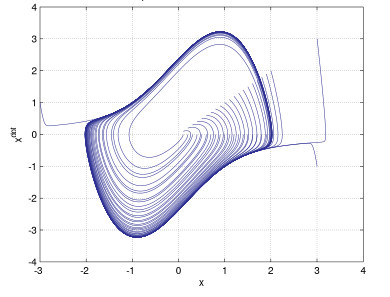
\includegraphics[width=.5\linewidth]{figures/Limitcycle}
    %\caption{Phase Space Diagram of a Van der Pol Oscillator. The attractor is indicated by the thick line and the trajectories by thin lines, all converging towards the attractor. \cite{phase}}
    %\scalebox{0.25}{0.25}
    %\label{fig:Limitcycle}
%\end{figure}
\tikzset{%
  %>={Latex[width=2mm,length=2mm]},
  % Specifications for style of nodes:
            base/.style = {rectangle, draw=black,
                           minimum width=2cm, minimum height=.5cm,
                           text centered, font=\sffamily},
  activityStarts/.style = {base,rounded corners, fill=blue!20},
       startstop/.style = {base, fill=red!30},
    activityRuns/.style = {base, fill=green!30},
         process/.style = {base, minimum width=2.5cm, fill=orange!15,
                           font=\ttfamily},
    interchangableProcess/.style = {base, minimum width=2.5cm, fill=yellow!15,
                           font=\ttfamily}
            %arrNote/.style = {draw=black, minimum width = font=\sffamily},
}
\begin{figure}[ht]
    \scalebox{1.35}{
        \begin{tikzpicture}[node distance=3cm, every node/.style={fill=white, font=\sffamily}, align=center]
        \node (pBounds)[activityStarts, scale=.5]{Parameter Bounds};
        \node (pInit)    [activityStarts, scale=.5, right of=pBounds, xshift = 2cm]{Parameters:\\initial guess};
        \node (system)          [activityStarts,scale=.5, right of=pInit, ]        {System};
        \node (dBounds)[activityStarts, scale=.5, right of=system, xshift =3cm]{Disturbance \\Bounds};
        \node (rInit)   [activityStarts,scale=.5, right of=dBounds]{$R_{curr}$:\\inital guess};
        \node (setParam)[interchangableProcess, scale=.5, below of= system, xshift = -2cm]{Apply Parameters to System};
        \node (compAttr)[process, scale=.5, below of= setParam, yshift = -3cm]{Compute Attractor};
        \node (samplDist)[process, scale=.5, below of=rInit, xshift=-2cm]{Sample Disturbances at $R_{curr}$};

        \node (simSys)[interchangableProcess, scale=.5, below of=samplDist]{Simulate Disturbed System};
        \node (eval)[interchangableProcess, scale=.5, below of=simSys]{Evaluate Convergence};
        \node (updR)[process, scale=.5, below of=eval]{Update $R_{curr}$};
        \node (rerm)[process, scale=.5, below of=updR, xshift=-6cm, yshift=1cm]{$R_{curr}=$ Robustness Measure};
        \node (opt)[process, scale=.5, below of= pInit, xshift = -4cm, yshift = -4cm]{Sample Parameters\\(via Optimizer)};

        \coordinate (join1) at ([yshift=-.5cm]pInit.south);
        \coordinate (join2) at ([yshift=-.5cm]rInit.south);
        \coordinate (join3) at ([yshift=-.47cm]updR.south))
        \coordinate (join4) at ([xshift=2cm]join2);

        \draw[->]   ([xshift=.25cm]pBounds.south) -| ([xshift=-3cm]opt);
        \draw[->] (join1) -| ([xshift=-2.2cm]setParam);
        \draw[-] ([xshift=2cm]opt) |- (join1);

        \draw  (pInit.south) edge (join1);
        \node (sysPar)[ scale = .4, left of=join1, xshift = 1cm]{System\\Parameters\\$\mathbf{s}_{\mathsf{P}}$};

        \draw[->] (system.south) -| ([xshift=7cm]setParam);
        %\node (adSys)[scale = .4, below of=setParam, yshift = -.75cm]{Adapted System};
        %\draw[-] (setParam.south) |- (adSys);
        %\draw[->] (adSys) |- (simSys.west);
        %\draw[->] (adSys) -| (compAttr);

        \draw[->] (setParam.south) |- node(adSys)[scale=.4]{Adapted System}(simSys.west);
        \draw[->] (adSys.south) -| (compAttr);
        \draw[->] (compAttr) -- node[scale=.4]{Attractor}(eval.west);
        \draw[->] (dBounds.south) -| ([xshift=-4cm]samplDist);
        %\draw[->] (rInit.south) -- node(R)[scale=.4]{$R_{curr}$}([xshift=10cm]samplDist);
        \draw[-] (rInit.south) |- (join2);
        \node (R)[scale =.5, below of=join2, yshift =3cm]{$R_{curr}$};
        \draw[->] (R.south) -| ([xshift=3.3cm]samplDist);
        \draw[->] (samplDist) -- node[scale=.4]{Disturbances\\$\{\mathbf{s}_{D,i}\}, i=\{1,2,...,n_s\}$}(simSys);
        \draw[->] (simSys) -- node[scale=.4]{State Trajectories}(eval);
        \draw[->] (eval) -- node[scale=.4]{$R_{curr} >$ or $<$ \\than minimal radius}(updR);
        \node (R2)[scale =.5, below of=join3, yshift =2.25cm]{$R_{curr}$};
        \draw[-] (updR.south) |- ([yshift=-.2cm]join3);
        \draw[->] (R2.west) |- (rerm.east);
        \draw[->] (rerm.west) -| (opt.south);
        \draw[-] (R2.east) -| (join4);
        \draw[-] (join4) -- ([xshift=.3cm]join2);\end{tikzpicture}
    }
    \caption[Framework Block Diagram]{Block diagram of the implementation of robustness measure computation and optimization. The blue boxes represent inputs specified by the user. The arrows connecting boxes designate the flow of data. Orange and yellow boxes correspond to operations on the data; the latter need to be specified for different systems and disturbances while the former stays as is. Outputs are defined depending on the application.}
    \label{fig:framework}
\end{figure}
\newpage
\subsection{Computing Trajectories} \label{solver}

One of the most difficult parts of the implementation is computing the state trajectories of the system. 
Finding an explicit analytical solution to the IVP is possible for simple cases, but very hard if not impossible for more complex systems. Numerical solvers represent a general approach to approximate the trajectories. For this the differential equations of the IVP are integrated over small time steps $\Delta t$ to approximate future states.
Iterating this process gives a discrete approximation of the continuous state trajectory. Note that general discrete points in time are represented as $t_n$.
The state trajectory is therefore just a set of states $\mathbf{x}(t_n)$ at time points $[t_0,t_1,\ldots, t_n]$ with $t_{i+1}-t_{i} = \Delta t\quad \forall\ i \in [0,n-1]\ $.
A smaller time step will result in a more accurate approximation, however it will take more computational effort to progress through the same amount of time.
It is advised to find a time step that is a sufficient compromise between accuracy and computational time and keeping it fixed from there on. Here $\Delta t = 0.01$ was found to be appropriate. 
Still numerical errors and will always be present, fundamentally limiting the precision that can be achieved. 

Solving the IVP only gives state trajectories of the isolated system through time.  Dynamics engines take this one step further by also taking friction and contact forces into account, simulating the interactions of the system with its environment. This addition is what allows for the direct application of disturbances to the system.

For this project CRL's Differentiable Dynamics Engine (DDE) was provided, doing most of the heavy lifting. %It simulates mechanical systems by considering multibody dynamics and contact forces. 
DDE represents the system states by generalized coorinates and provides the generalized accelerations $\ddot{\mathbf{q}}(t_n)$ in addition to $\mathbf{q}(t_n)$ and $\dot{\mathbf{q}}(t_n)$ for ever iteration of the trajectory. For any computation, an object describing the system to be simulated, the time step $\Delta t$ and the initial state $\mathbf{x}_0 = \begin{bmatrix} \mathbf{q}_0&\dot{\mathbf{q}_0}\end{bmatrix}^\intercal$ are required. Contact forces are modeled using spring dampener elements, the dynamics of which depend on the time step, which is another reason for keeping it constant between different test. Another particularity to keep in mind is the choice of y as the vertical axis, while x and z lie in the horizontal plane. 
%(anything else important to note?)
 %Choose a time step that's too large and the results will become inaccurate, choose it too small and large computations will become infeasible. A compromise has to be found.


%The solution to the IVP can be found using numerical solvers. This is not an explicit solution but the trajectory must be iteratively computed by integrating the differential equations over small time steps. 

%Here we used dde ... write some stuff about dde.

%Describe what dde puts out
    %DDE provides q, qdot and qddot at every timestep when computing the trajectories. 




%dde does most of the work, we just have to define the attractor and see if the trajectory converges. 

%Starting with a sytem of ODE's and as corresponding set of initial states, the first step towards computing robustness measure is finding the resulting trajectories. This is achieved by numerically integrating the differential equations over small timesteps until either convergence is detected or the $t_max$ is reached. With the chosen solver it is imperative to keep this timestep constant when comparing different robustness measures. The time step has a direct influence on the solvers accuracy and by that onto the system dynamics. 

%trajectories here are not continuous but sets of states for discrete timepoints . 


\subsection{Detecting Attractors} \label{attractors}

In order to evaluate the convergence of a trajectory resulting from a disturbance, first the attracting set of states must be found. For this the nonlinear dynamics definitions ar followed for a general approach.

%!! Note that we generally want to run the undisturbed simulation a bit so it can settle. 
%Automatic identification of fixed points

When setting up a simulation, especially when compliance is present, the undisturbed initial state resulting from the construction is rarely part of an attractor. To remedy this simulations of the undisturbed system should be run to let the state trajectory settle to a valid attractor. As in section \ref{attractortheory}, fixed points and limit cycles handled separately. The approaches are exemplified by a 1d spring mass element. 

In the case of fixed points, it suffices to check every state along the computed trajectory for the fixed point condition \ref{eq:3}. Whith DDE checking this is trivial as the generalized accelerations $\ddot{\mathbf{q}}(t_n)$ are provided. 
The first state at time $t_n = t_{fp}$ for which $\dot{\mathbf{q}}(t_{fp}) = \mathbf{0}$ and $\ddot{\mathbf{q}}(t_{fp}) = \mathbf{0}$ hold, can be saved as an attractor in the form of $\mathbf{x} = \begin{bmatrix}\mathbf{q}(t_{pf})&\mathbf{0}\end{bmatrix}^\intercal$, for disturbed trajectories to be compared to. 
If $\ddot{\mathbf{q}}(t_n)$ is not eailsy obtainable, one may check a number of states $\mathbf{x}(t_n),\ t_n\ >\ t_{pf}$ for $\dot{\mathbf{q}}(t_n) = \mathbf{0}$. This does not guarantee that state $\mathbf{x}(t_{pf})$ is a fixed point, 
but it makes it more probable the more additional states are checked. 
%If the state $\norm{\mathbf{x}(t_{pf})}$ is smaller than some chosen error tolerance.  

\begin{figure}[h]
\centering
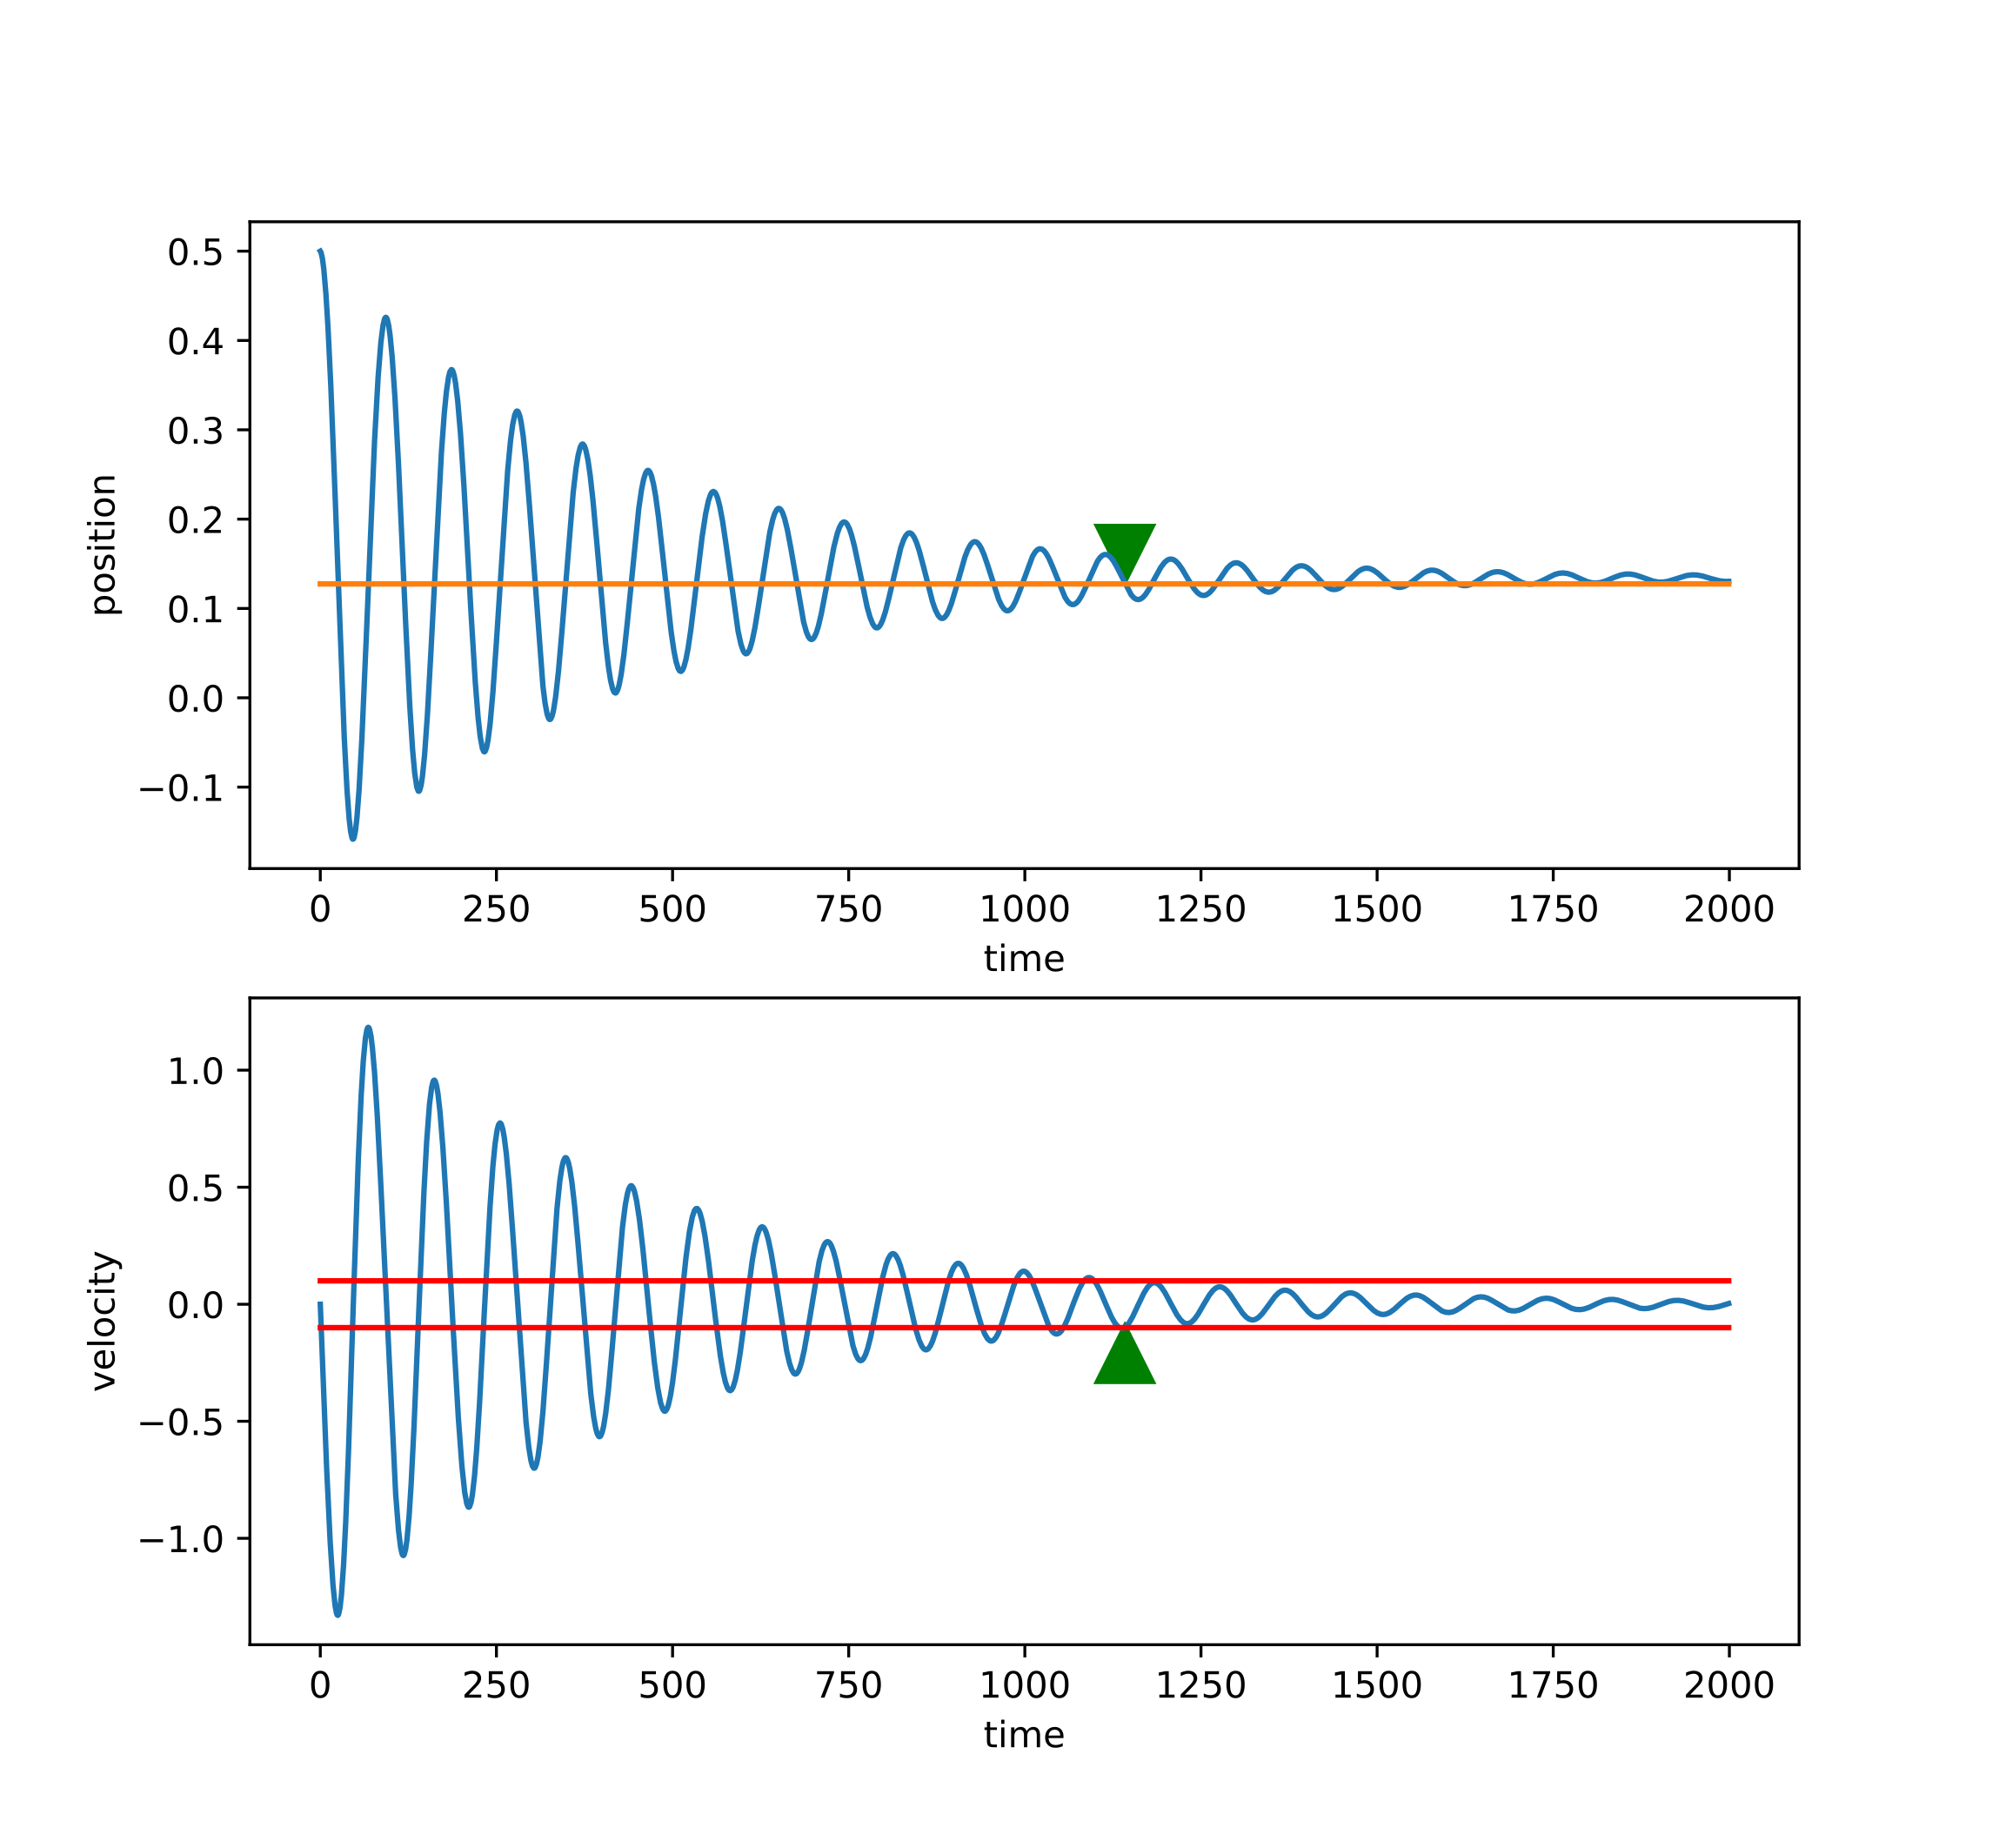
\includegraphics[width=.7\textwidth]{figures/fixed_point_detection.png}
\caption[Fixed Point Detection]{Detection of the fixed point of a 1d spring mass element. Once the velocity is below the tolerance(red) for all future times, indicated by the green triangle, the position at that time point is taken as the attractor (orange). A slight deviation from the true fixed point remains.}
\label{fpdet}
\end{figure}

Finding limit cycles is a bit more challenging as they may show chaotic behaviour and because of the discretization of time, aliasing effects could arise. For practicality the following assumptions are made. 
First the forcing period $T$ of the system is chosen to be an integer multiple of the time step $T = m\cdot \Delta t, m \in \mathbb{N}$ to mitigate aliasing. In addiontion the period of the limit cycle is assumed to coincide with the period of the forcing period that causes the periodic behaviour in the first place. So if a controller is tasked to move a leg in a periodic fashion, it is assumed that the actual end effector trajectory shows that same period, without phase shift. Note that this is not true generally and needs to be verified. 
In this scenario one can apply the conditions for a limit cycle \ref{eq:5} in continuous time to the discrete case directly.
If a state $\mathbf{x}(t_n) = \mathbf{x}(t_n+T)$ is found, the set of states $\{\ \mathbf{x}(t_n) \mid t_n \in [t_i,t_{i+1},\ldots,t_i+T]\ \}$ can be saved as the attractor. Denote $t_{lc,0}$ as the time where the trajectory first reaches the limit cycle. To rule ot numerical errors one may want to verify the attractor by choosing one period of states after the initial occurance of the attractor and compare each and every state $\mathbf{x}(t_{lc,0}+i\Delta t) = \mathbf{x}(t_{lc,0}+i\Delta t+T)\ \ \forall\ i \in \{1,2,\ldots, m-1\}$.

\begin{figure}[h]
\centering
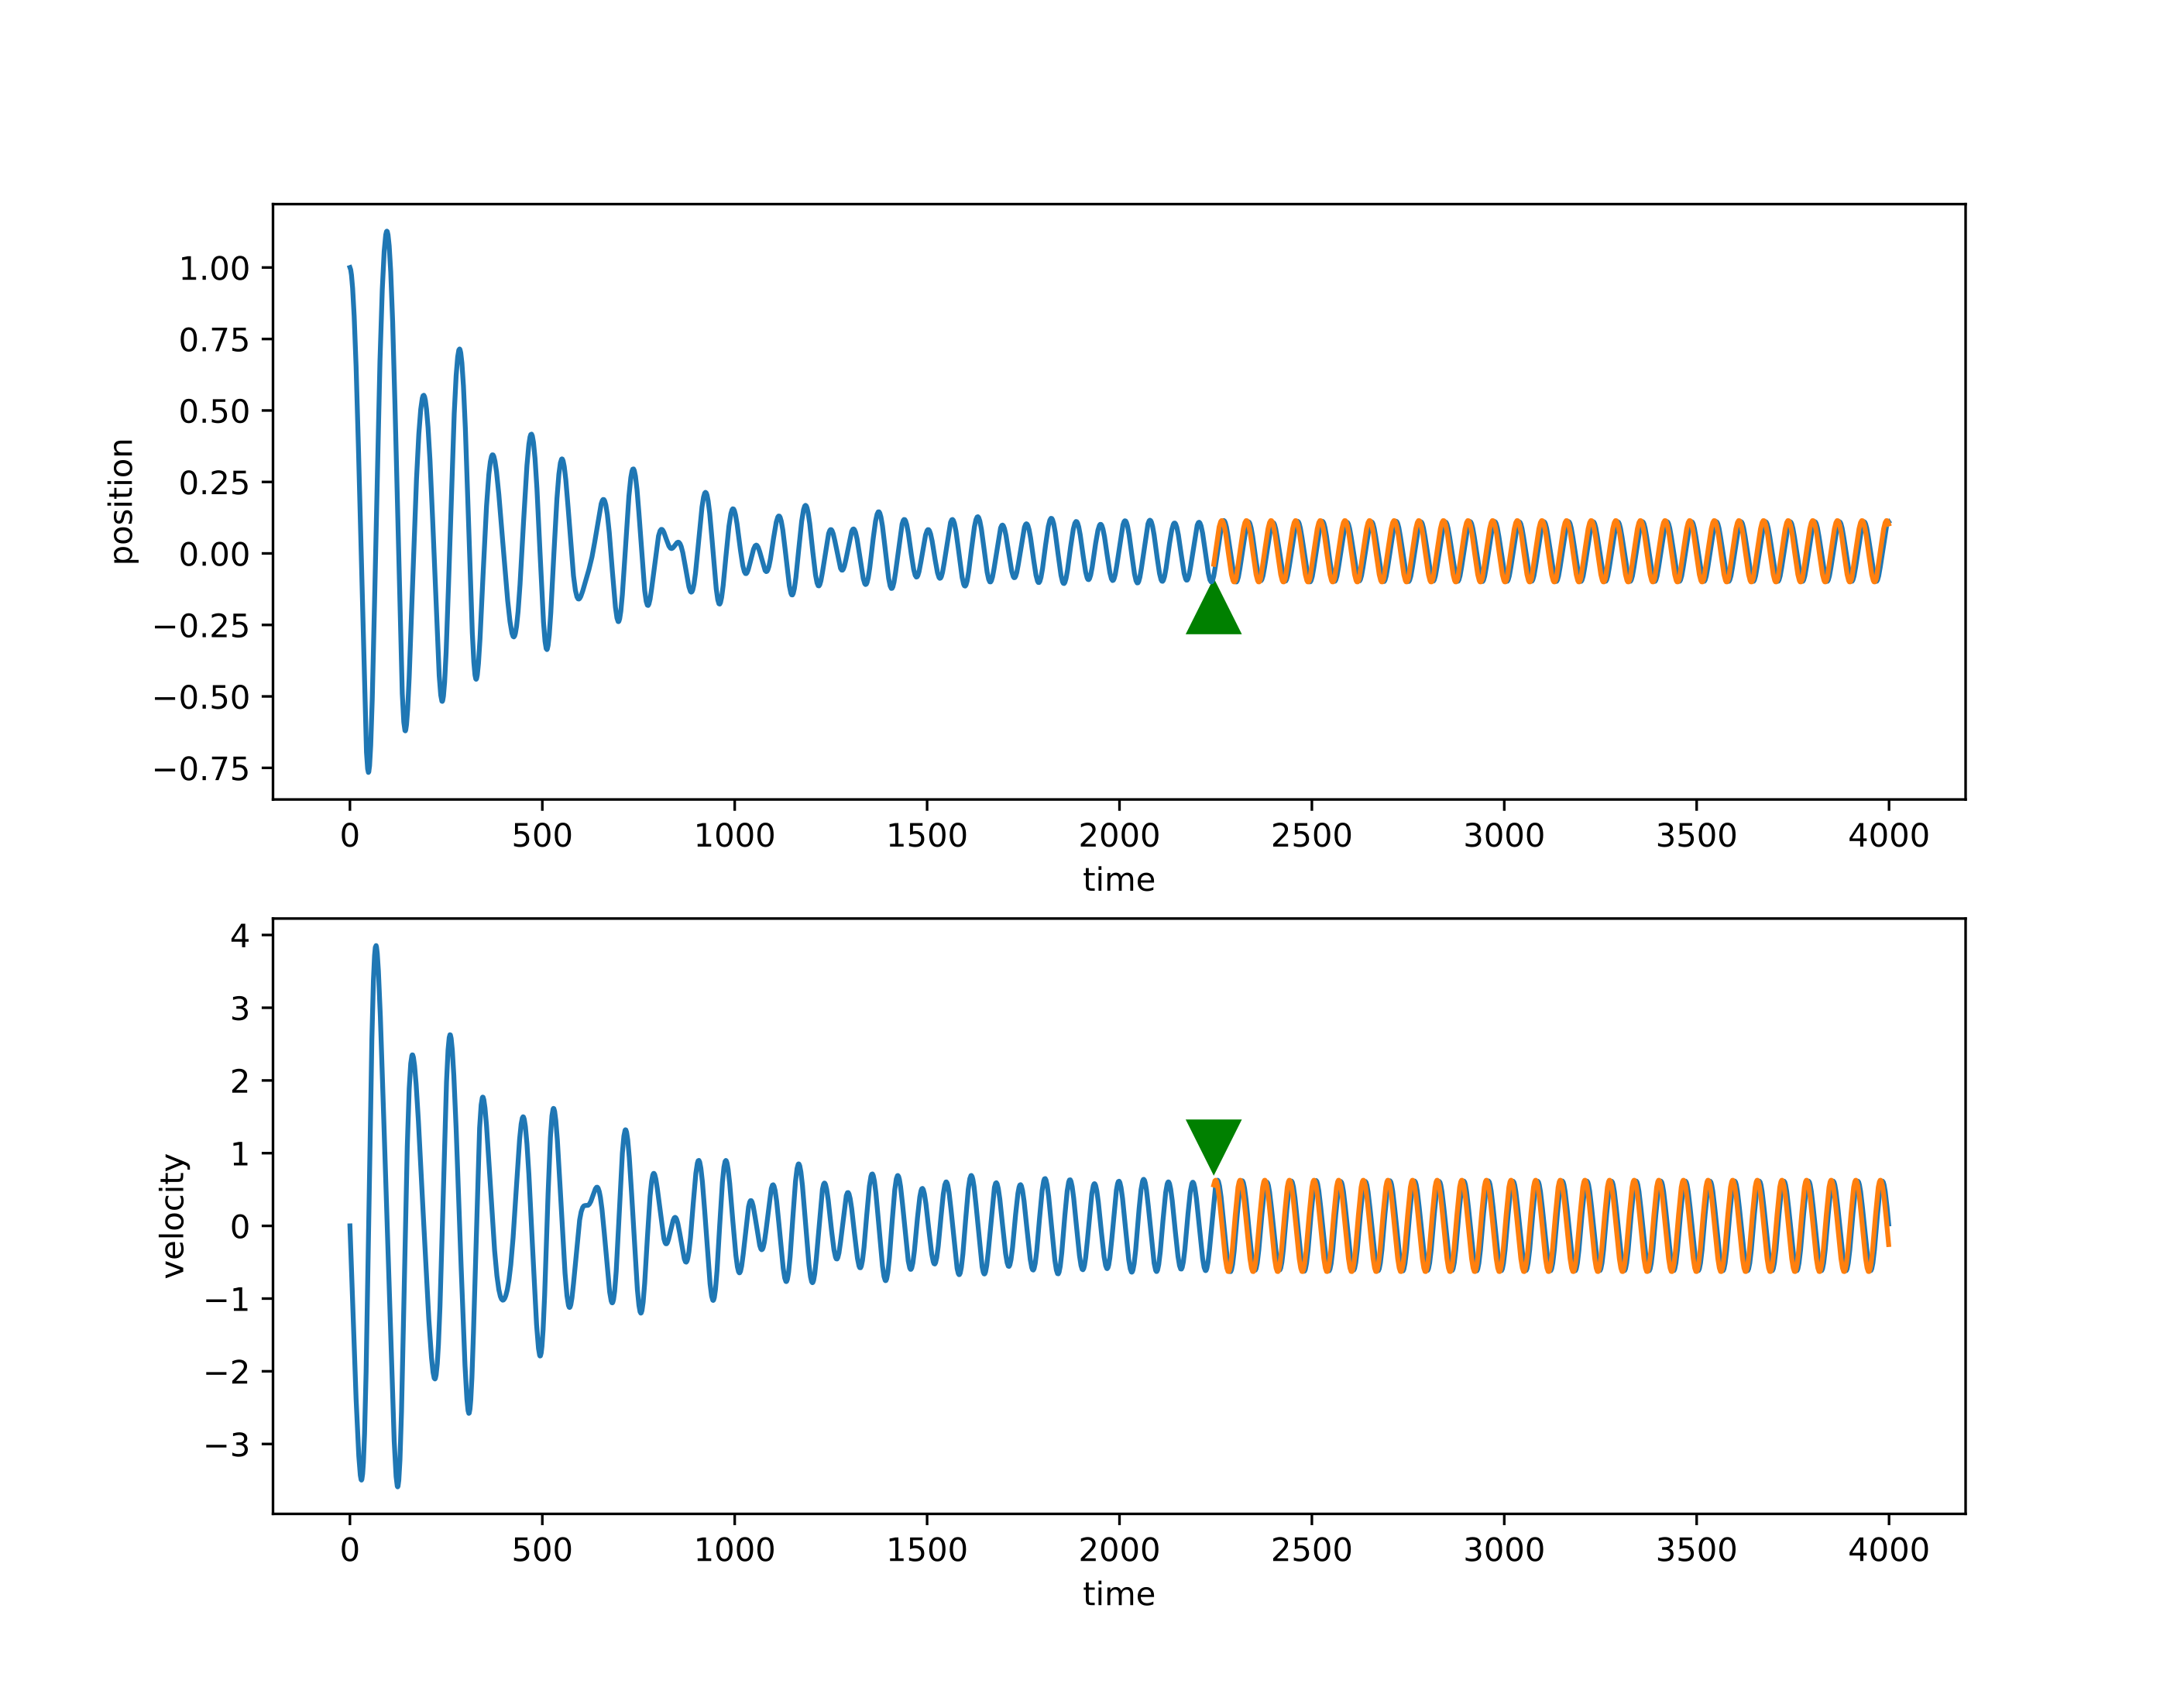
\includegraphics[width=.7\textwidth]{figures/limit_cycle_detection.png}
\caption[Limit Cycle Detection]{Detection of the limit cycle of a forced 1d spring mass element. An oscillating forcing is applied to the system, which is why it will always stay in motion, settling into a the limit cycle (orange). It is detected once positions one period in future time are close enough to the current position, indicated by the green triangle.}
\label{lcdet}
\end{figure}

Another approach for detecting limit cycles tested is recasting the problem such that it is equivalent to finding a fixed point. For systems with a dominant oscillation of a particular coordinate, this can be done using Poincare Sections. The idea here is to reduce the trajectory by sampling states at period of the oscillation. This essentially removes the oscillations and the fixed point condition can be applied to the reduced trajectory. This approach is well-founded in the theory of dynamical systems, however it is infeasible once there exist oscillations along multiple coordinates. In addition because of the reduction, much longer trajectories are needed, ultimately increasing computational effort, which is why this approach is not recommended. 

Note that when comparing two states $\mathbf{x}$ and $\mathbf{y}$ numerically, checking for equality can give misleading results because of rounding errors. It is rather suggested to check $\mid\mid \mathbf{x} - \mathbf{y} \mid\mid\ < \epsilon$, for some small positive $\epsilon$ and some vector norm $\mid\mid\cdot\mid\mid$. For the norm, the root mean square error \begin{gather}\mid\mid \mathbf{x} - \mathbf{y} \mid\mid_{_{RMSE}} = \sqrt{\frac{1}{n}\sum_{i=1}^{n}(x_i-y_i)^2},\quad \mathbf{x},\mathbf{y} \in \mathbb{R}^n\end{gather}was used. This approach is reflected in Figures (the two above, that have yet to be created) by error margins. 

It is also important to inspect the resulting attractor. As generally there exist multiple attractors in any phase space, it has to be verified that the detected attractor does represent the correct undisturbed behaviour. In initial testing a square cloth model (see figure \ref{fig:invcloth}) made up of mass spring elements was made dynamic by applying oscillations at the top two corners. When computing the limit cycle for this system, the detected attrator seemed to be shifted from its expected location (oscillations about the "hanging down" position). Visual inspection using a graphical interface for dde showed, that for some initial condition, the entire cloth stabilized in the inverted position, which was reflected in the detected attractor. This effect is known from inverted pendulums, where applying oscillations stabilizes the inverted position (figure \ref{fig:invcloth}). This exemplifies the need for verification.  

\begin{figure}[h!]
    \centering
        \begin{minipage}{0.3\textwidth}
            \centering
            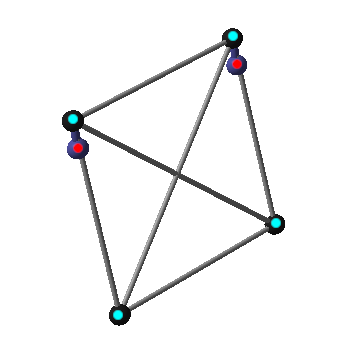
\includegraphics[width=\textwidth]{figures/noninverted_cloth_col_small.png} % second figure itself
            %\caption{second figure}
        \end{minipage}
        \begin{minipage}{0.4\textwidth}
            \centering
            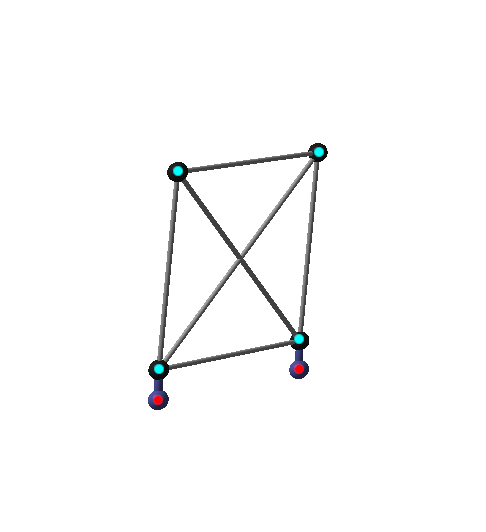
\includegraphics[width=\textwidth]{figures/inverted_cloth_col_small.png} % first figure itself
            %\caption{first figure}
        \end{minipage}\hfill
        
        
        \begin{minipage}{0.4\textwidth}
            \centering
            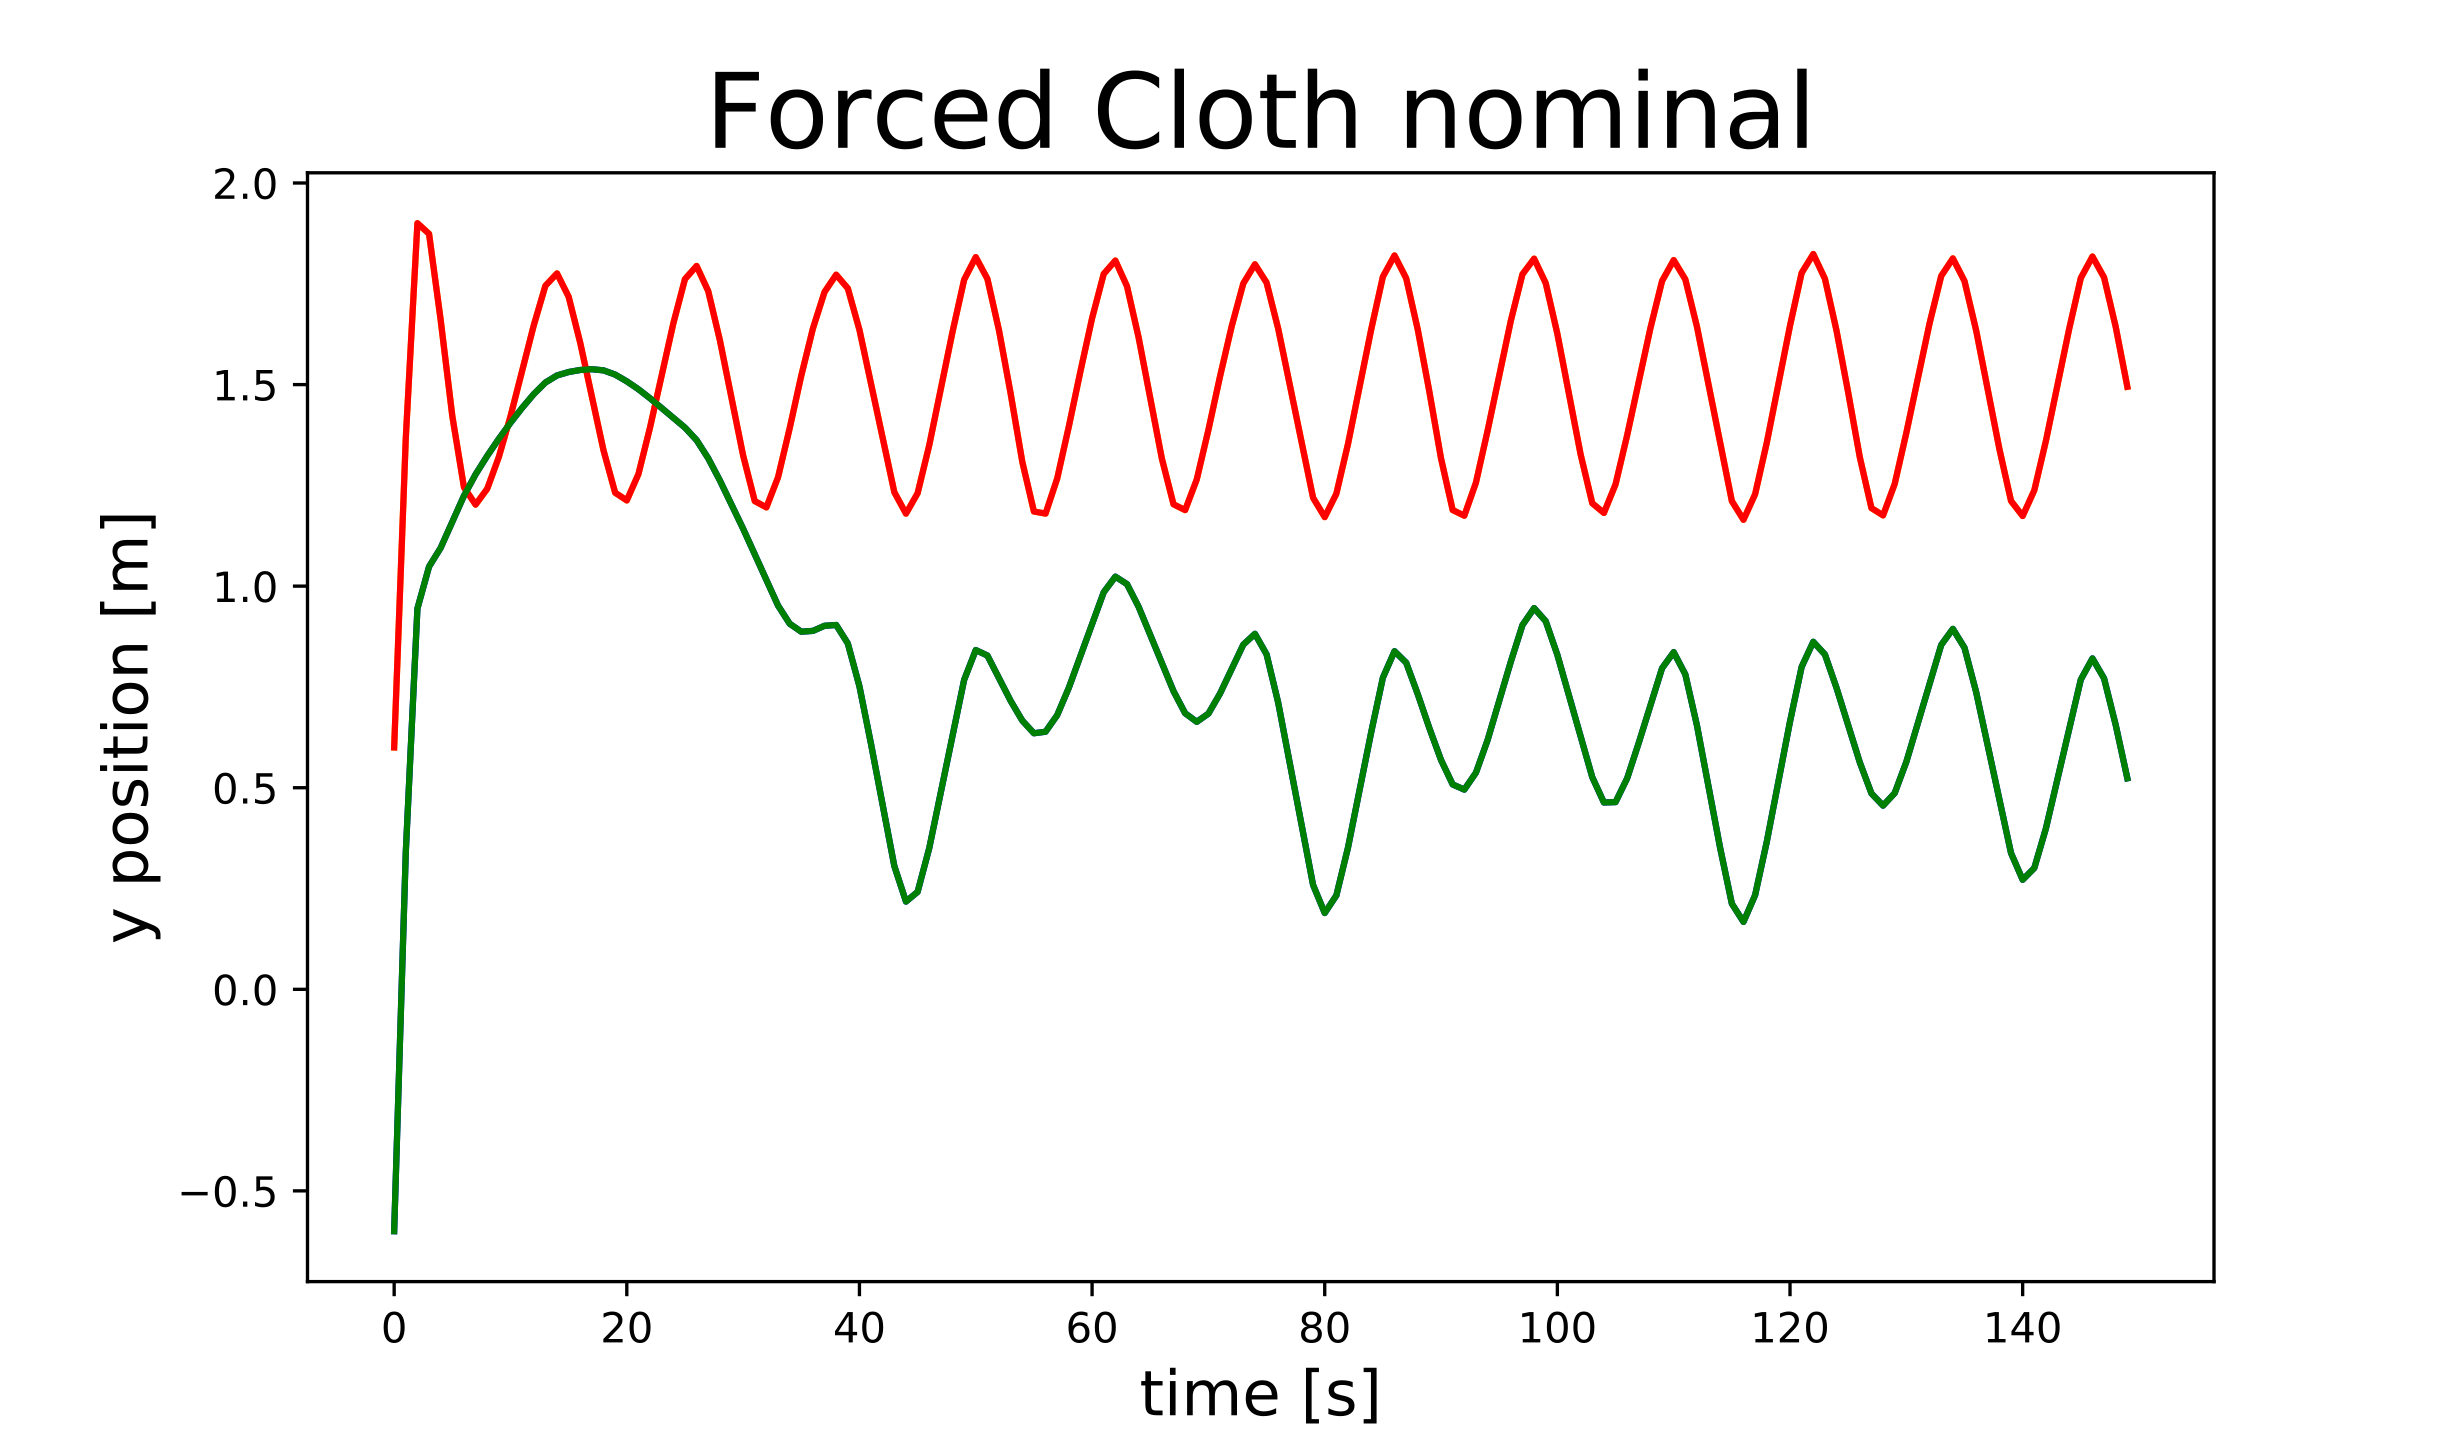
\includegraphics[width=\textwidth]{figures/forced_cloth_nominal_graph.png} % second figure itself
            %\caption{second figure}
        \end{minipage}
        \begin{minipage}{0.4\textwidth}
            \centering
            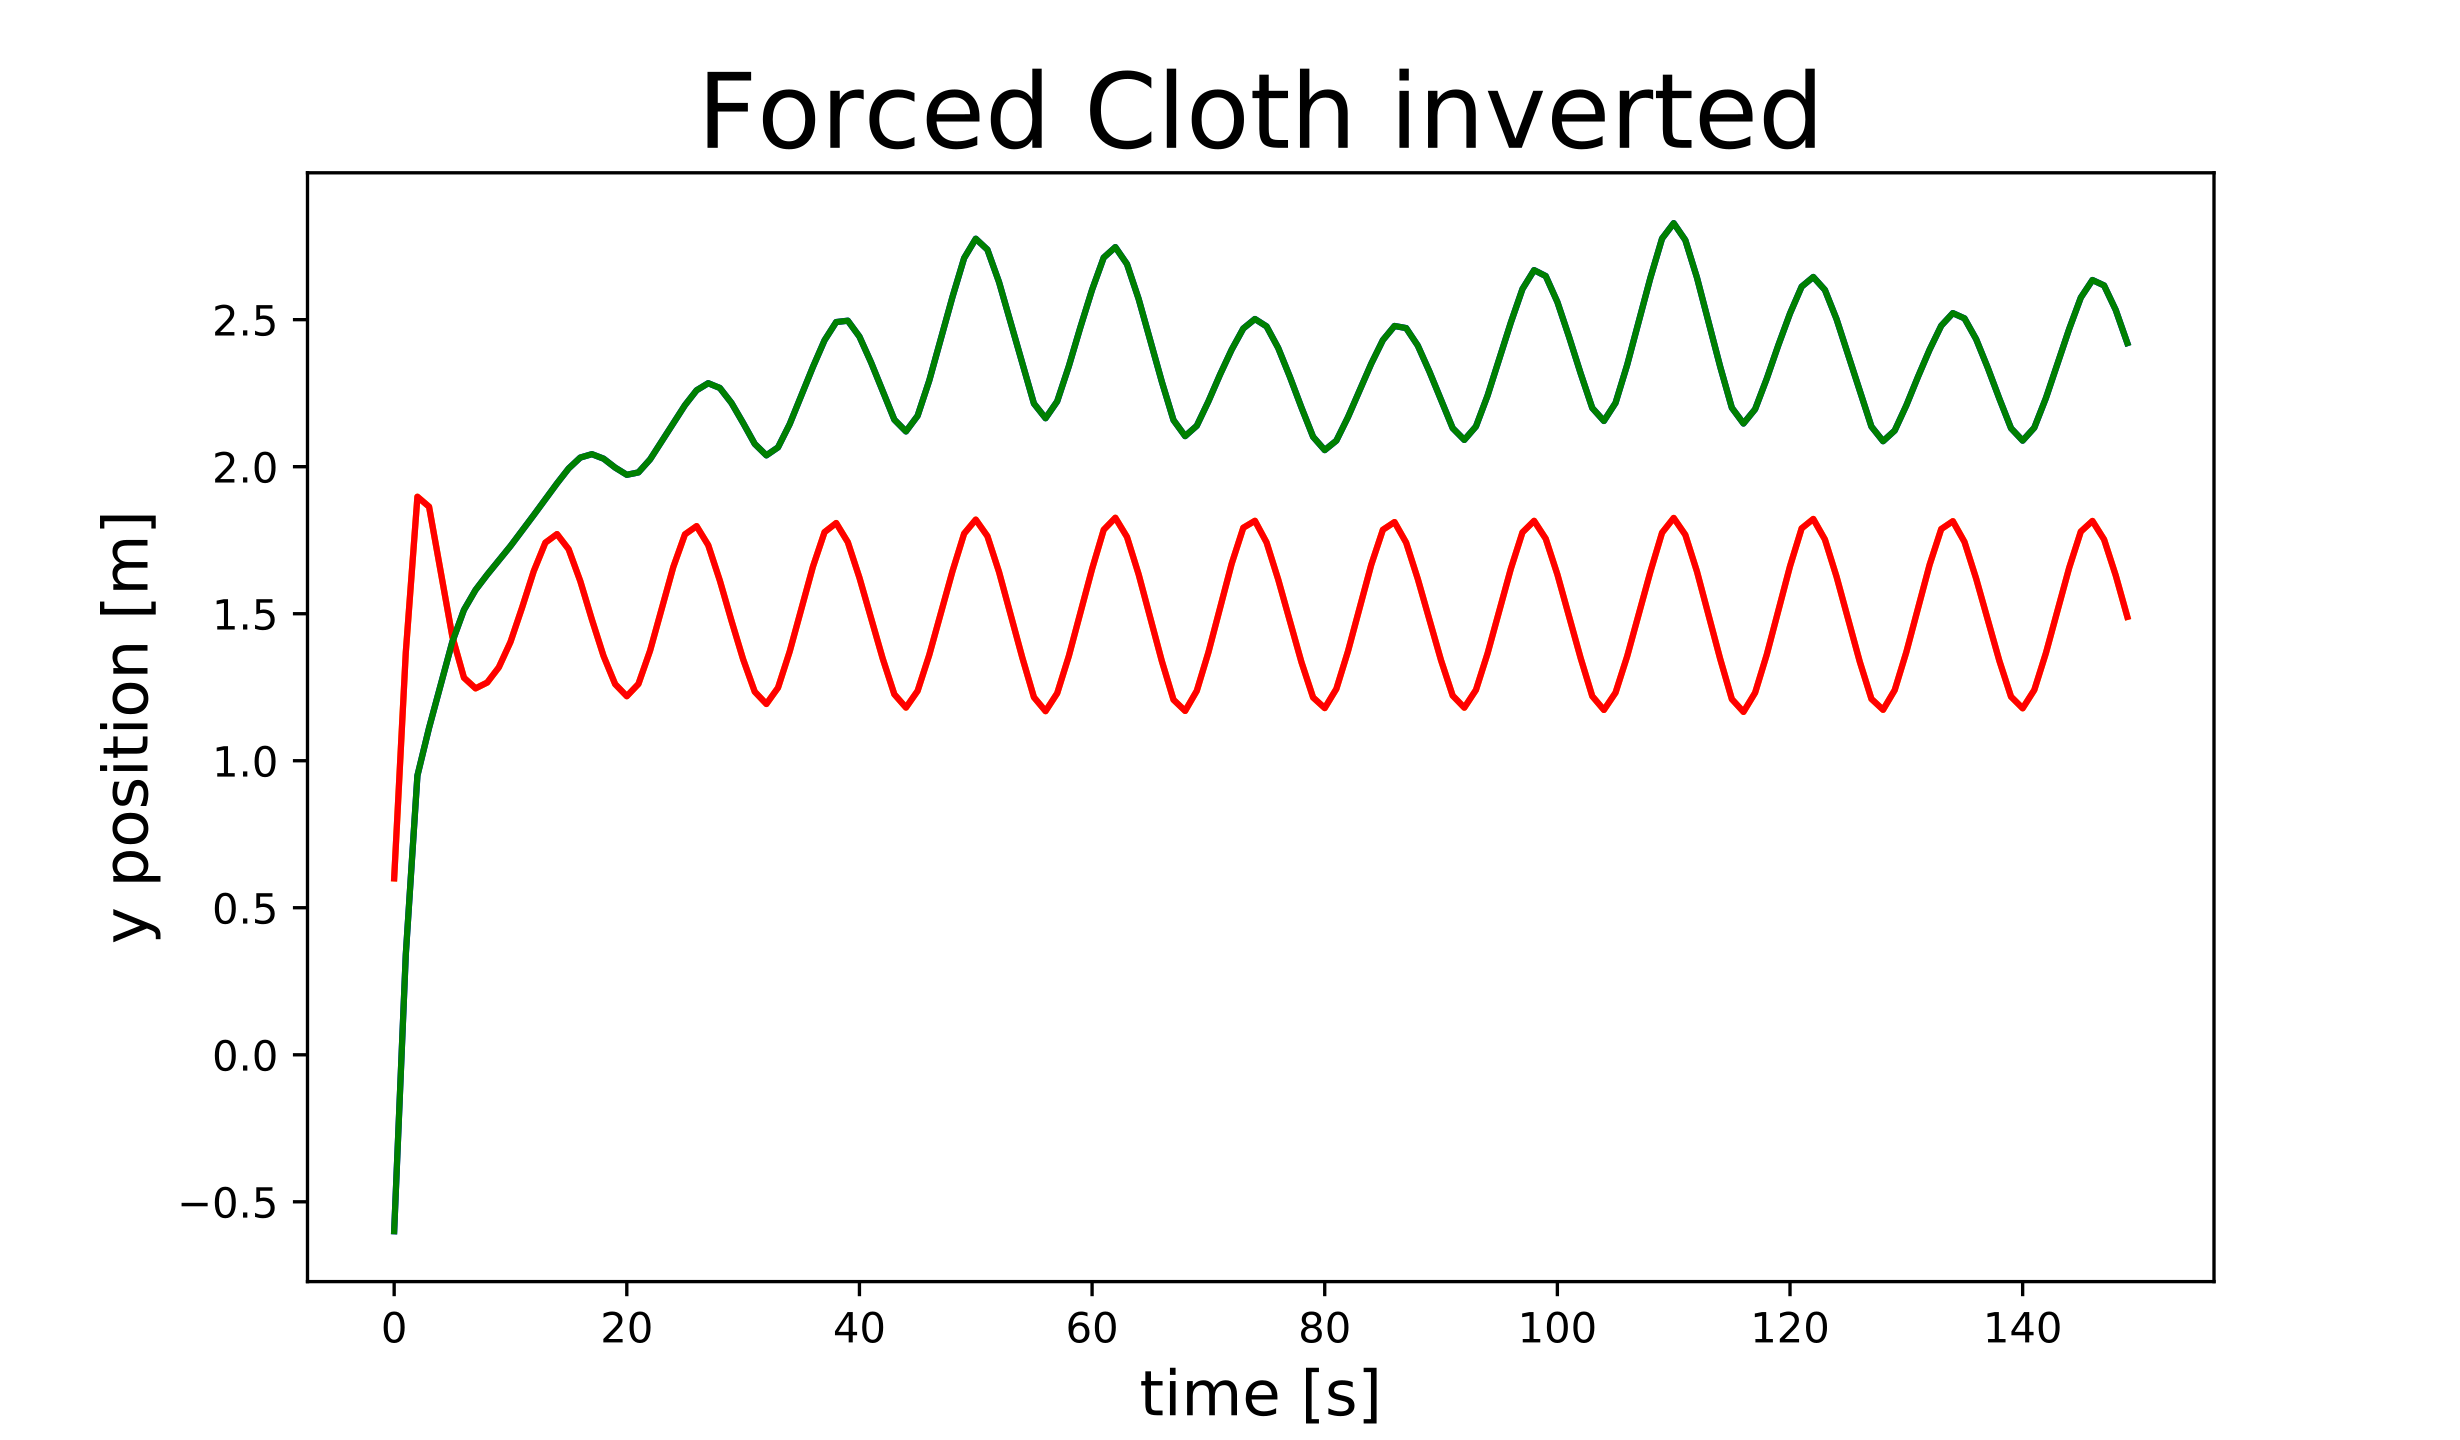
\includegraphics[width=\textwidth]{figures/forced_cloth_inverted_graph.png} % second figure itself
            %\caption{second figure}
        \end{minipage}

    \caption[Example for systems with multiple attractors: Inverted Cloth]{Example for a system with multiple attractors. A cloth model consisting of pointmasses (blue dots) connected by springs is oscillated via two handels (red dots). The hanging down position is found to be a limit cycle, seen by the periodic motion of the position of the pointmasses. The inverted position is also a limit cycle, where the previously lower point masses (green graph) are now top.}
    \label{fig:invcloth}
\end{figure}

For certain systems and application, fully determining all coordinates of the attractor might turn out to be difficult or simply excessively precise. Examples of this are found in section \ref{app}.
%Once we detect a state at time $t = t_{fp}$ for which $\mathbf{q}(t_{fp}) = \mathbf{0}$ and $\dot{\mathbf{q}}(t_{fp}) = \mathbf{0}$ hold, we can save this state as an attractor for disturbed trajectories to be compared to. In order to rule out numerical errors, we can additionally check that for the generalized accelerations provided by DDE $\ddot{\mathbf{q}}(t_{fp}) = \mathbf{0}$ holds, implying that the state $\mathbf{x}(t) = \begin{bmatrix}\mathbf{q}(t)&\dot{\mathbf{q}}(t)\end{bmatrix}^\intercal$ will stay $\mathbf{0}$ for future times as well. Alternatively one could verify that any  

    %Fixed points
    %this is rather easy
    %ixed points are defined states where $\dot{\mathbf{x}}(t) = \mathbf{0} \quad \forall \ t\  >\  t_0 $, i.e. $\mathbf{q}(t)=\mathbf{q}_{fp}, \dot{\mathbf{q}}(t) = \ddot{\mathbf{q}}(t)  \forall t > t_0$

    
    %Periodic Orbits
    %    not as trivial. need assumptions
    %    assume that period of attractor is the same as forcing frequency. Think controller forcing a gait given period, then the leg will also move at that period. This is not generally true and needs to be verified. 

\subsection{Evaluating Convergence} \label{convergence}
    
    Given an attractor, evaluation of convergence simply follows definition $\ref{eq:5}$. Clearly trajectories cannot be computed for infiite future times, however by definition $\ref{eq:2}$, it can be deduce that if a state $\mathbf{x}(t_{conv})$ lies on the attractor, all future states $\mathbf{x}(t_n),\ t_n > t_{conv}$ will as well, fullfilling the definition of convergence. 
 Evaluating convergence therefore simplifies to finding a state on the trajectory that coincides with an element of the attractor at any point in time. If undisturbed after $t_{conv}$, the state should stay on the attractor for all future times. This holds for all types of attractors. Similar to the attractor detection, additional states $\mathbf{x}(t_n),\ t_n>t_{conv}$ should be verified to also be on the attractor to make the results more robust to numerical errors. If future disturbances will be applied or disturbances are continuous, future states need to be verified until either the disturbances or the simulation itself stops, i.e. $t_{max}$ is reached. 

 These approaches are heavily based on the nonlinear considerations outlined in sections \ref{dynamicstheory} and \ref{attractortheory}. Ultimately, how one determines whether the system converges to the attractor under disturbances may be implemented in any fashion that works. Specific coordinates maybe be selected to be tracked as indicators of convergence if the system allows for it. Ulitmately, one may come up with many case specific simplifications, just as for the detection of attractors. 

\begin{figure}[h]
\centering
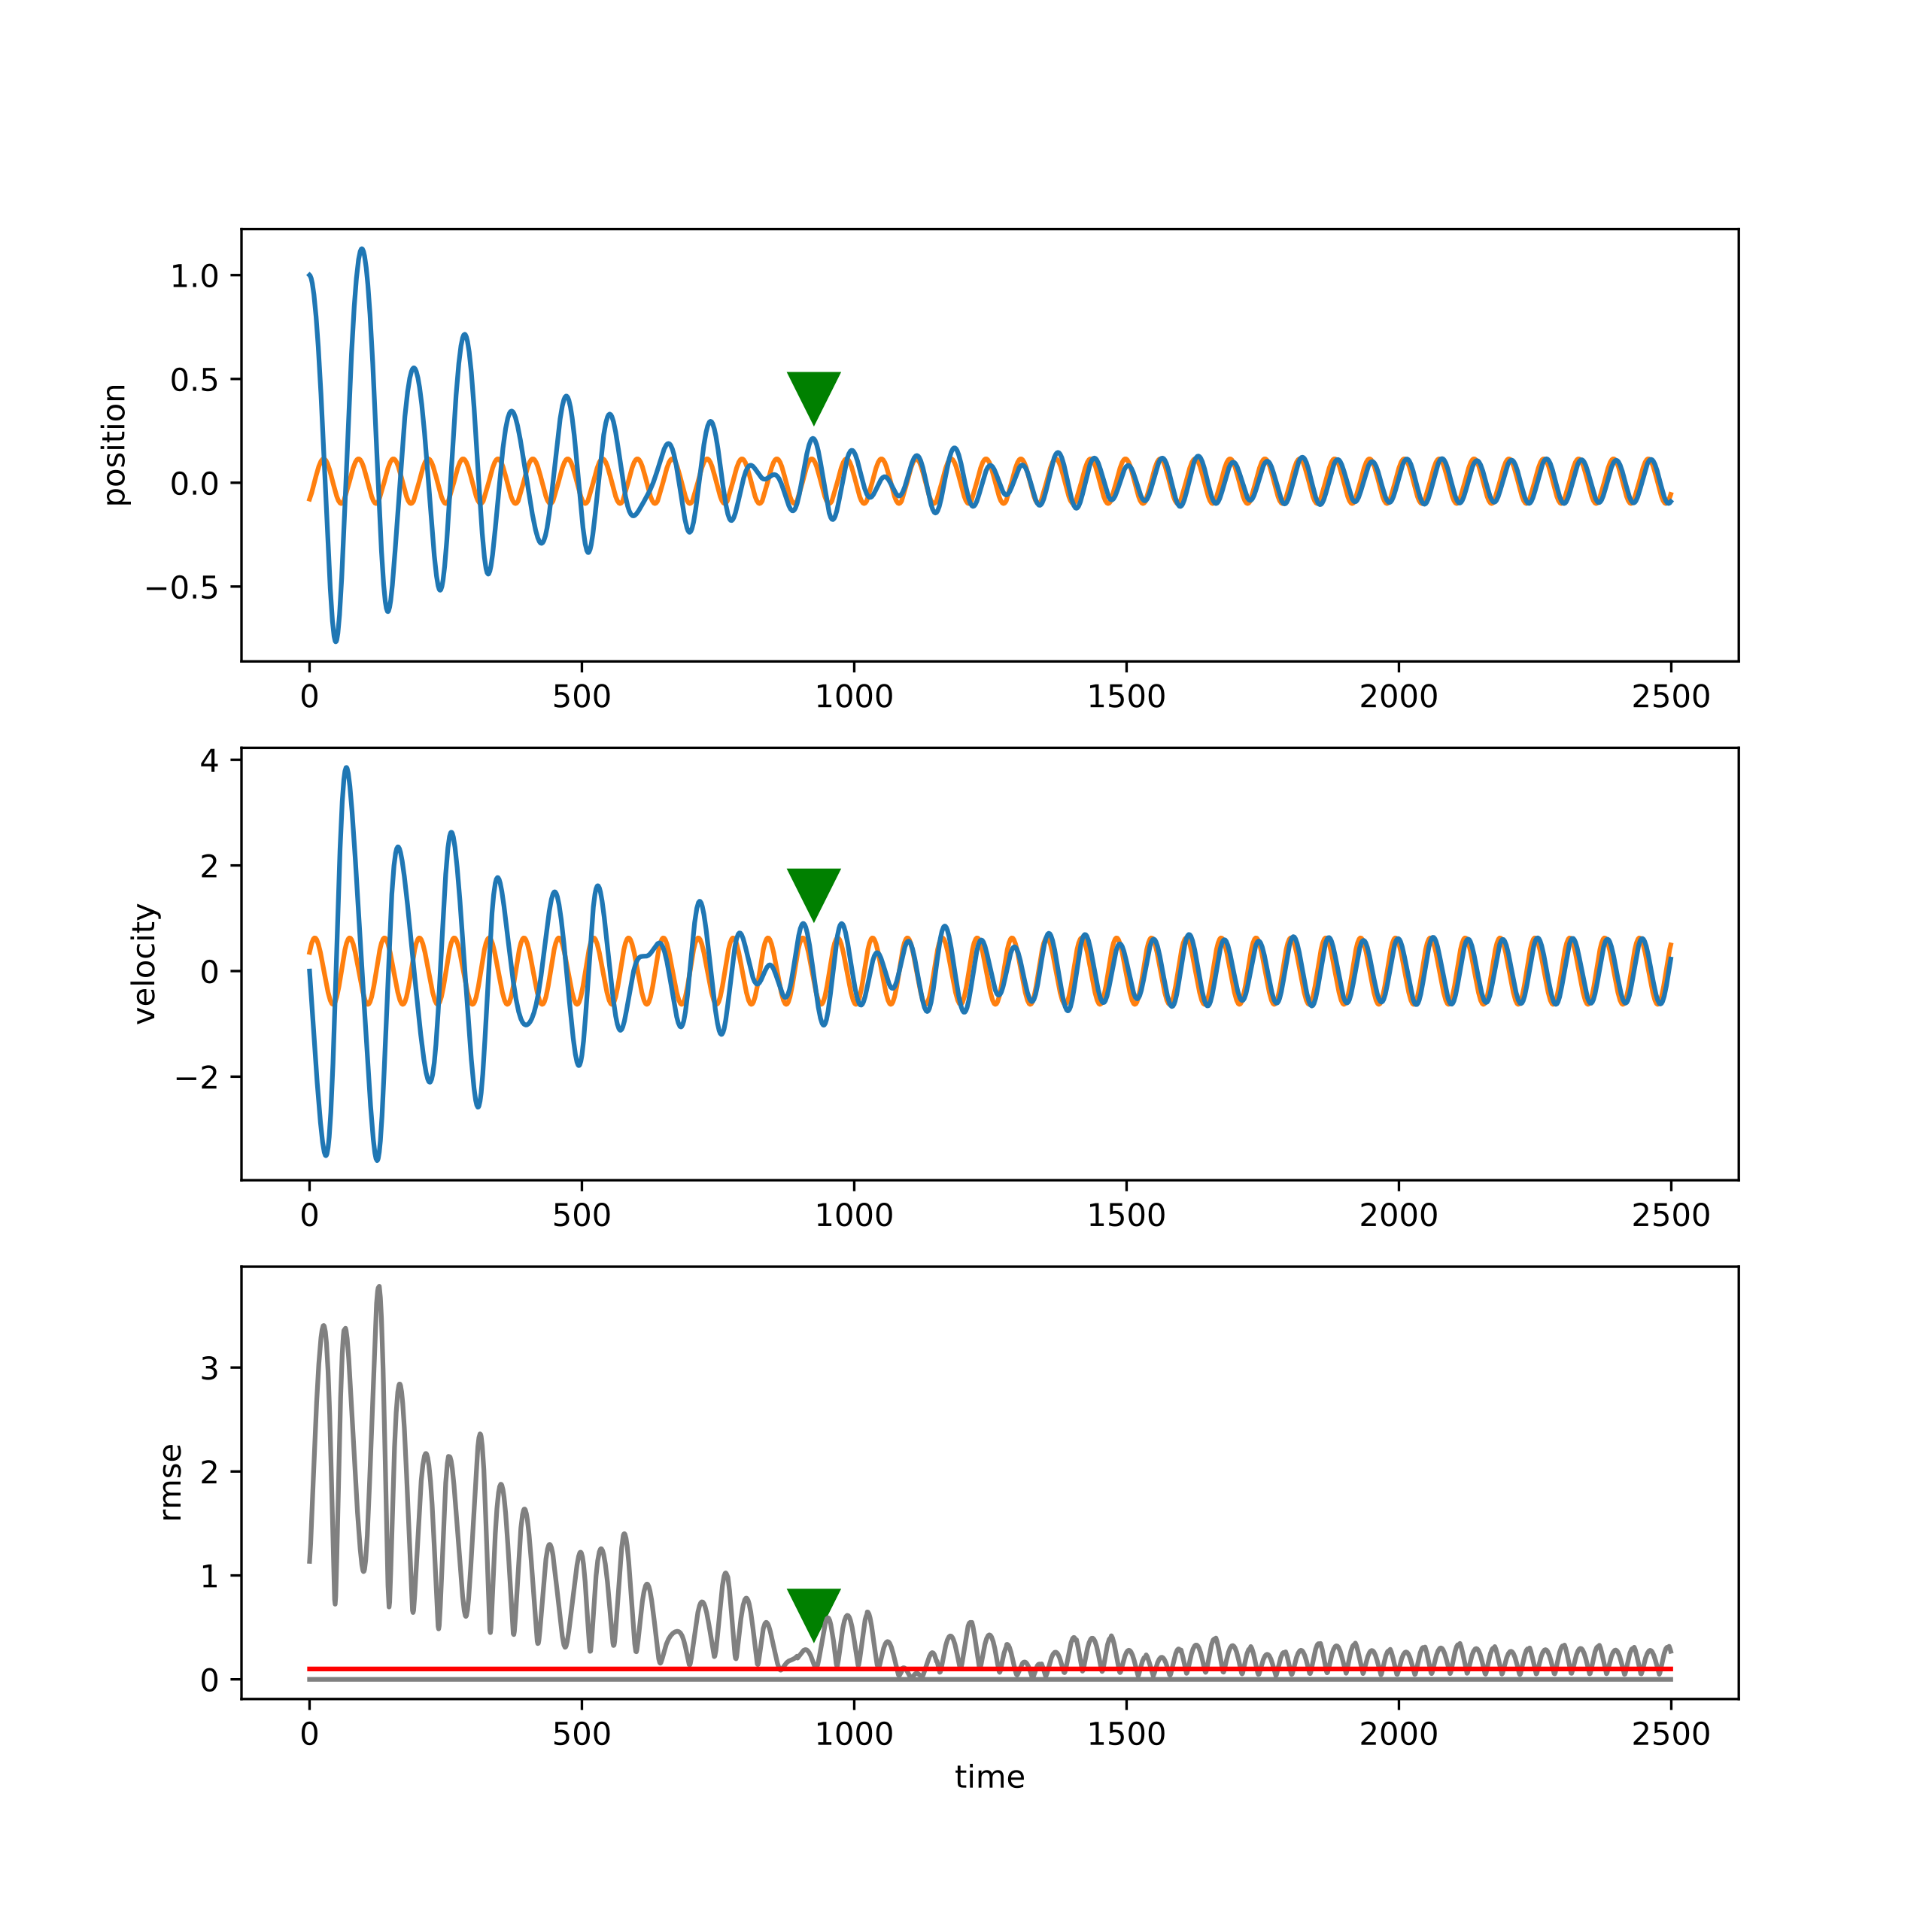
\includegraphics[width=.7\textwidth]{figures/limit_cycle_convergence.png}
\caption[Convergence to Limit Cycle]{Convergence of a disturbed forced 1d spring mass element. An attractor (orange) is given. Once the state of the system is close enough to any state in the attractor, characterized by the rmse (grey) being below a tolerance (red), convergence is detected. The time of convergence is indicated by the green triangle. The rmse does go above the tolerance periodically, but always returns.}
\label{lcconv}
\end{figure}

 %Also that with high DOF systems, as there are many different coordionates, small errors might add up in the norm and convergence following (REF) is never detected. 


  

%especially in multibody dynamics it might suffice to only track the generalized coordinates of one body, the core for example. This needs to be decided on a case by case basis. 
%Relate this to laikago, as we don't care about the particulat leg pose, as long as the robot does not tip over. 

%The nonlinear dynamics approach with evaluating convergence of the system state to the attractor will always work in theory (enough computational power and precision), but ultimately, if there exists a computationally simpler way to decide whether the system recovers from disturbances, it should be chosen over the rigorous approach. 
 

    %In many cases, one can and might even want to loosen the requirements for convergence. Ultimately this needs to be decided on a case by case basis, but some examples shall be demonstrated here.  
    
    %sometimes we can loosen the requirements for convergence. For the laikago experiments, where the goal is just for the quadruped to not tip over, we only check height of the core above ground and it's orientation. 
    
    %Issue that this is one specific state that does not accomodate for any deviation. With laikago standing up, we might accept translations of the robot in the xy-plane or rotations about the 

    

    %In real world applications, it is often not enough for a system to return to the desired states 
    %Cleary it is impractical to let t go to infitiy, which is why some $t_{n,max}$ needs to be defined at which the simulation stops. 

    %Would be enough to check the state if it is similar to an element of the attractor. But as we might still have disturbances being applied, we should check future states as well. For a twist

    %Any way of checking and guaranteeing for non convergence (divergence) may be simpler. it actually really useful, as when continually apllied at every timestep, the simulation can be stopped if divergence is detected and computational time be saved. Example Laikgao, if we want it to stand upright and we detect it tipping over, that run has clearly failed and can be stopped early. 
    %quite similar to 



    %The nonlinear dynamics view is uesful in detecting attractors and evaluating, but sometimes when the needed information can be acquired more easily, we always chose that route. 

\subsection{minRad Algorithm} \label{minrad}
    
    %Goal: 
    %Intro
    %Describe minRad algortithm and how previous sections play in.
    %Talk aboubt finding the parameters (nSamples and nIterations, effects)

    %MinRad encompasses .. from the framework
    With the tools outlined above one can evaluate the response of a system to any individual disturbance. In order to finally copmute the robustness measure, one needs to measure the minimal radius of the set of converging disturbances as defined in \ref{robustnessmeasure}. We approximate this value following \ref{fig:alg}, applying the bisection algorithm to an initial upper guess $R_{curr} =  R_{max,init}$ and iteratively updating $R_{curr}$ until the desired accuracy is reached. For any iteration, $n_{s}$ number of disturbances are randomly sampled on the surface of the d dimensional hypersphere of radius $R_{curr}$ in $\mathsf{D}$. This achieved by enforcing $\mid\mid \mathbf{s}_{\mathsf{D}}\mid\mid\ = R_{curr}$ for all samples at that iteration. For any $R_{curr}$, if it lies below the true minimal radius, all disturbances ${s_D}$ sampled at $R_{curr}$ and applied to the underlying system will result in convergence. Conversely, a single failure to converge indicates that the true minimal radius must be smaller than $R_{curr}$. The bisection algorithm requires an inital lower bound as well, but as the minimal radius $R_m$ must by construction always be positive, 0 is a generally valid choice here. 

    As the algorithm is bisecting the domain of possible values at every iteration, one can compute the resolution $h$ of the resulting robustness measure after $n_i$ iterations as: $h = R_{max,init}\cdot\frac{1}{2}^{n_i}$. The choice of $n_i$ depends on the overarching application of the robustnes measure, i.e. how much precision is required.The other parameter to be considered is the number of samples $n_{s}$ at every iteration. The sampling is stochastic in nature, so no determenistic results can be guaranteed. A $n_{s}$ that is too low might miss some disturbances that result in divergence of the system, leading the algorithm down a wrong path. High $n_{s}$ on the other hand lead to an unnecessary increase in computational effort. An exemplary comparison can be seen in figure \ref{fig:minradcomp}. 
    $n_{s}$ should be chosen in a way that with a set number of iterations, the resulting robustness measures are consistent when computed repeatedly. 

    \begin{figure}[ht] 
    \centering
    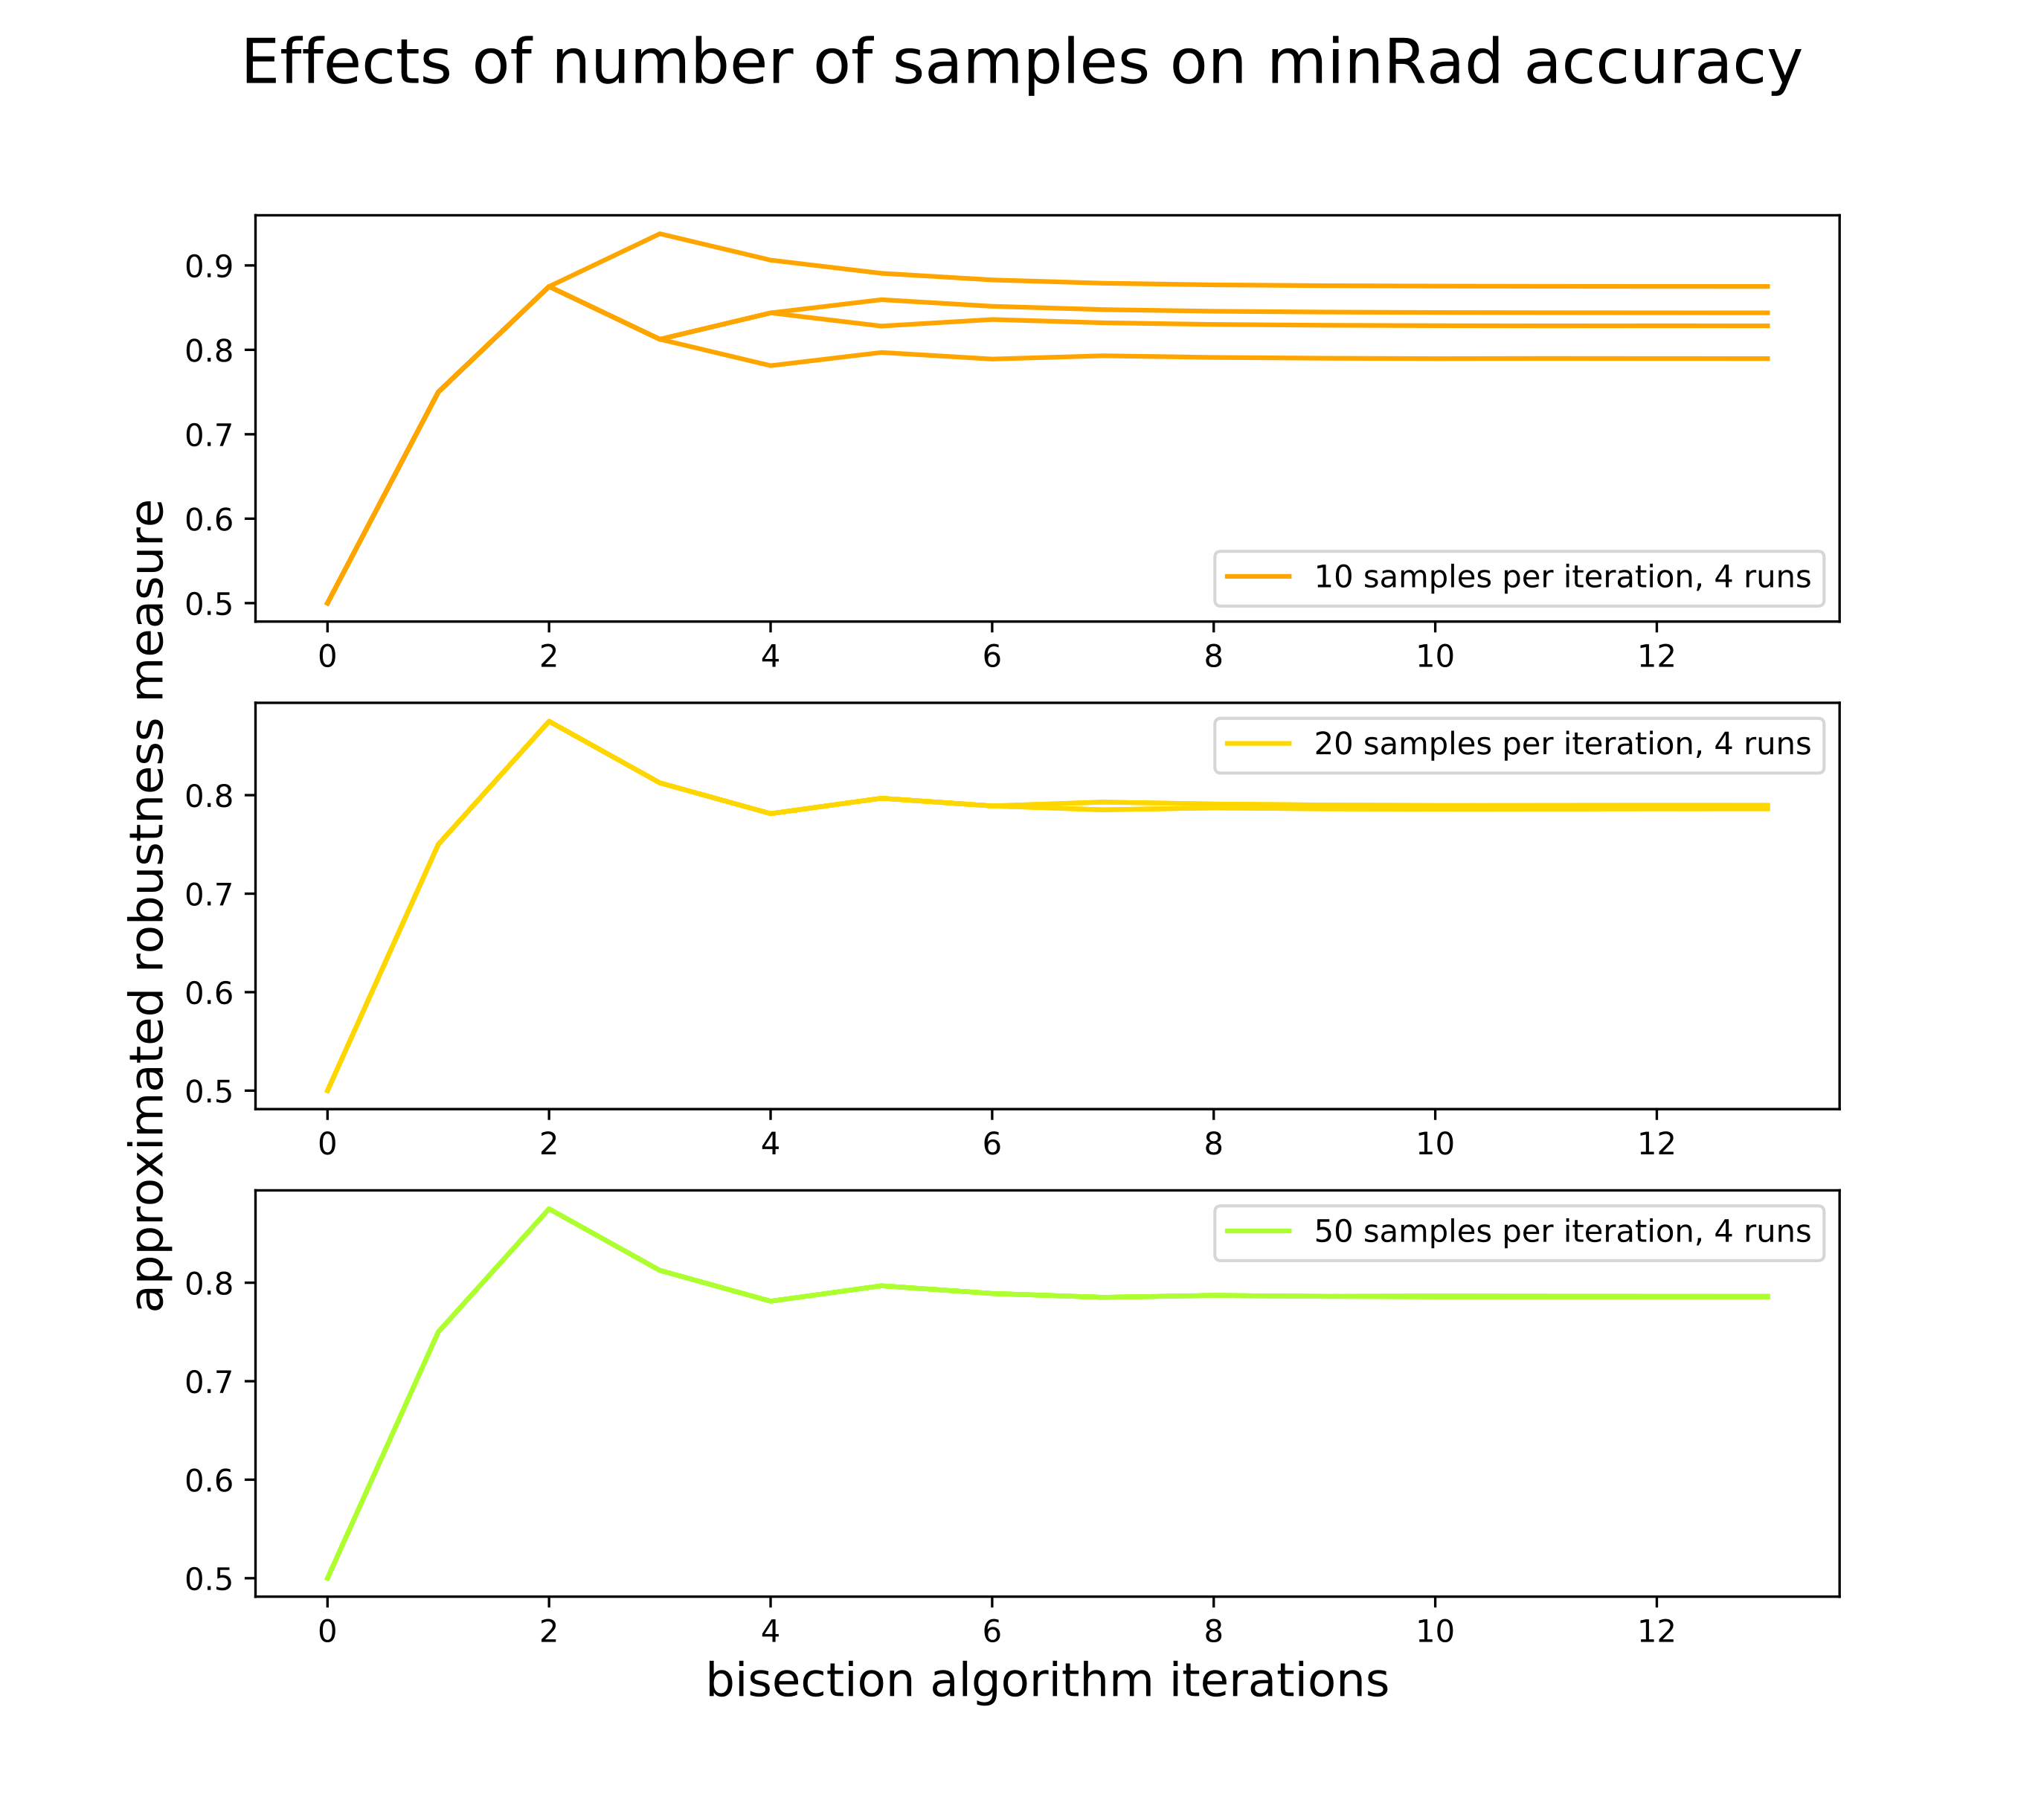
\includegraphics[width=.9\linewidth]{figures/minRad_tuning_graph.png}
    \caption[minRad Tuning]{Exemplification of the effect of sample size on the precision of the minRad algorithm. More samples result in higher precision when computing many iterations, however for lower number of iterations low sample numbers are suffitient as well.}
    \label{fig:minradcomp}
    \end{figure}

    Monotonic evolution of $R_{curr}$ over all iterations indicates issues. If $R_{curr}$ monotonically decreasing, it implies that it is always larger than the true minimal radius. Here either $R_{max,init}$ needs to be decreased or the number of iterations increased. On the other hand, monotonical increase implies $R_{max,init}$ was chosen too small.

    As the scaling of the dimensions in $\mathsf{D}$ w.r.t. each other has significant, the algorithm was implemented for a general case. Given a $d$ dimensional $\mathsf{D}$ and lower and upper bounds $b_{low,i}, b_{upp,i} \in \mathbb{R},\ i \in \{1,2,\ldots,d\ \}$ for every dimension, the domain is restricted to $[0,1]$ for the minRad algorithm, and scaled up to $[b_{low,i}, b_{upp,i}]$ when applying the disturbances for the system. $\mathsf{R_{max,init}}$ was always set to 1, restricting $\mathsf{R_{curr}}$ to $[0,1]$ and giving different robustness measures some degree of comparability. 
    Changing to a different $\mathsf{D}$ then only requires definining it's dimensionality and corresponding boundaries.

    %(verifying minRad results by discretizing disturbance space and brute force exploring the space by evaluating every single node. )
    %By guessing and checking Whether any guess lies below or above the actual minimal radius, 
    %For this we chose the bisection algorithm with monte carlo sampling from REF.

    %(the graphic for the bisection algorithm would probably already be in previous work. I feel like it would be better located here?, also I guess we don't use the same one as we are applying it to $\mathsf{D}$)

    %maybe not go into too much detail on how it works (look at ref)
    
    %While the minimal radius is already a strong simplification from fully measuring the set of recoveries, finding it is nontrivial. The bisection algorithm is a way of approximating it. We choose an initial guess that we expect to be sure for it to be larger than the minimal radius. Then we randomly sample disturbances in the ds that have a norm equating the current radius guess. 
    %For any given radius we can determine whether it is larger or smaller than the actual minimal radius by sampling a suffitient number of disturbance samples on the hypersphere with that radius and 

    %If the system recovers from all disturbance samples, we conclude that we haven't reached the boundary and we %increse our guess (insert formula). If even just one doesn't recover, we shrink the guess as there are clearly regions where the basin boundary lies closer than the current guess.   

    %Because of the random sampling of disturbances, the convergence of the minRad algorithm and therefore the robustness value is inherently stochastic and might be dominated by noise. The extent of theis noise can be reduced by larger amounts of samples. An compromize between noise and computational time must be found.

    %Number of iterations
    
    %tuning. For this it maks sense to look at a discretized version of the 
    %here it should be noted that if the algorithm increases or decreases monotonically, the results should be disregarded, as either the initial guess was already smaller than the minimal radius or the boundary of the set of recoveries was not yet reached. consequence: either larger initial max guess or more iterations.

    %visualizations
    %plot resultion as a function of iterations. NO, write down the formula $resolution = (1/2)^n$ with n being the number of iterations. 
    %Plot variance as a function of nsamples for some example. 

\subsection{Multithreading} \label{mt}
    
    %computational time can be reduced by 
    The computation of the state trajectories takes up a bulk of the computational time. As for every minRad iteration a number trajectories need to be found, this process benefits from parallelization. A simple multithreading pipeline was implement, computing $n_{th}$ simulations on $n_{th}$ threads in parallel. For this to be effitient, it is necessary for the functions to give feedback to the pipeline on whether the simulations are done. Completed simulations are restarted with different disturbance samples until either all $n_s$ samples are computed or an instance of divergence is detected. In this case all threads are stopped and the minRad algorithm proceeds to the next iteration. 
    With this the computational time can approximatiely be reduced by a factor of $n_{th}$, assuming there exist $n_{th}$ cores on the platform. 

\subsection{Optimization} \label{opt}
    
    %Given a way to quantify the robustness of a system and the possibility to change its parameters, it is possible to optimize said parameters to maximize robustness.
    At this point it is possible to change the system parameters in order to increase its robustness measure.
    Without applying any further algorithms, one may discretize $\mathsf{P}$ in every dimension and compute the robustness for every possible combination of parameter values $\mathbf{s}_{\mathsf{P}}$. The optimal parameters $\mathbf{s}_{\mathsf{P},opt}$ are the ones with the maximal robustness within the resolution of the chosen discretization step size $h$. This approach is computationally expensive and becomes infeasible for high dimensional $\mathsf{P}$ as the computational effort is $\mathcal{O}(\frac{1}{h^p})$ with smaller $h$ yielding higher precision and $p$ being the dimension of $\mathsf{P}$. 
    
    A second approach is utilizing optimizers, which can drastically reduce the number of robustness computations needed to get (close) to an optimum. As derivatives of the robustness measure are not available, the choice fell on evolutionary algorithms. In particular, the Covariance Matrix Adaptation Evolution Strategy (CMAES) was used with algorithm parameters being kept as suggested by the documentation. %Combining both approaches enables comparison and verification of either one. 


    %find out how the order of computational effort when making discretization smaller vs how much one bisection algorithm iteration can do. 
    %cmaes
    %given robustness value, any optimizer that does not depend on derivatives can be used. 
    %Of course one can also just explore the entire parameter space, howeve that is quite costly. Useful for debugging though (rough estimate if optimizer converges).

    %complexity reductions should probably be noted where they are implemented (i.e. not in this section)


\subsection{Boundaries of $\mathsf{D}$ and $\mathsf{P}$ } \label{bounds}

    The boundaries of $\mathsf{D}$ are relevant for the minRad algorithm during sampling of the disturbances. Because of their fundamental effect on the robustness measure, they have to be chosen thoughtfully. In the tests carried out $\mathsf{D}$ was restricted to 2 dimensions for simplicity and ease of visualization, making finding appropriate boundaries by trial and error feasible. This would be significantly more challenging for $\mathsf{D}$ with of higher dimensions. The approach was to find a balanced set of boundaries where at the minimal radius all elements $s_{\mathsf{D},i} = 0.5$, implying $R_{minRad} = \begin{Vmatrix}\mathbf{s}_{\mathsf{D}}\end{Vmatrix}= \sqrt{\sum_{i=1}^{d} s_{\mathsf{D},i}^2} = \frac{\sqrt{d}}{2}$ for some set of system parameters. These boundaries were then used when computing robustness measures for different sets of parameters. 
    Here it shall be noted that some elements of disturbance may be negative. In order to keep the framework simple, these cases are handled by randomly negating those values and scaling them appropriately. 

    %Here there could be an opportunity to have an influence on the eventual optimization process. Increasing the upper boundary of a specific dimension of $\mathsf{D}$ would shift the boundary of the set of recoveries closer to the origin. This squishing changes the shape of the set of recoveries and in turn affects the robustness measure. (this was already done in the first D-P space section)
 


    %s the boundaries on $\mathsf{P}$ and especially $\mathsf{D}$ are so fundamental, a few notes on their choice. 

    %D
    %As outlined in Section .. the scaling of the individual dimensions in $\mathsf{D}$ w.r.t each other has a significant effect on the resulting robustness measure. While this is problematic for a general notion of robustness, it can be leveraged to weight specific aspects of the disturbances, which will have a direct effect on system parameters optimized using the robustness measure. 
    %With this one could prioritize towards what the system should be especially robust against. 
    %In favor of universality, the entire minRad algortihm was implemented independetly from specific disturbance boundaries. For every dimension of D, the domain was chosen to be [0,1], $\mathsf{R_{max,init}}$ was set to one 
    %the robustness measure 

    %was noted in REF that it can be an ellipse as well, but they didn't know how to choose it's parameters. We do this by analysis and finding reasonable boundaries in the $\mathsf{D}$.

    %if disturbance coordinates can be negaive as well, assuming that they are symmetric about the origin, we just randomly negate those coorinates. 
    %All of this needs to be done manually anyways, so why not also put some thought into it 
    %changing even the unit changes the scaling and therefore the robustness value.
    %must choose something and see if it makes sense. 

    %sampling and minrad always on domain [0,1] in every dimension of D and then scale up to proper domain.
    %Sampling (idea that we sample within a d dim space where every dimension has domain [0,1], and then scale by boundaries chosen for every coordinate). 
    The boundaries of $\mathsf{P}$ dictate the possible range of parameters and are particularly relevant for the optimizer. Basic system functionality must be given within the boundaries as detecting the attractor is based on that assumption. They can often be found by considerations of the physical constraints or visual inspection of the system behaviour, if a graphical user interface is available.


    %that that the system must function more or less properly within them. This was also done by trial and error and 
    %for $\mathsf{P}$, it just needs to be tested what valid parameters can be. With laikago we found the smallest damping and stiffness for which it was still standing and chose those as bottom boundaries and took the maximum values possible as the top boundaries. 
    %This very much needs to be considered on a case by case basis. 







    
    


    %explain and give examples on how boundaries were chosen. 



    %for $\mathsf{D}$, bottom boundary is 0 if the disturbance coordinate is $\in \mathbb{R}_+$ (is the case in droptest). If disturbance coordinate is $\in \mathbb{R}$, i.e. can take negative values as well, the bottom boundary is the lowest. z

    %Top boundary


    


    

    %order of complexity depending on $\mathsf{P}$ and $\mathsf{D}$


    %for this a pipeline was implemented, simulating one sim on every virtual (?) core until all samples were processed, or all were stopped if any failed recovery was detected. With the system at hand this reduced computational time (for this part of the entire computation) by a factor of $n_{th}$. 
    %pseudocode or block diagram.)

\section{Application to a Quadruped Robot} \label{app}
    
    The framework was tested on the model of a 78 DoF quadruped robot "Laikago". Each of its four legs has 3 motors, two at the hip and one at the knee. The basic functionality provided was a standing pose which would be held by active position control of all 12 motors. This position control could be tuned with stiffness and damping parameters. These were the choice of system parameters to be optimized for robustness against disturbances. Two sets of disturbances were chosen with which two test were carried out, the "Drop Test" and the "Swing Test". 

    \begin{figure}[h!]
    \centering
    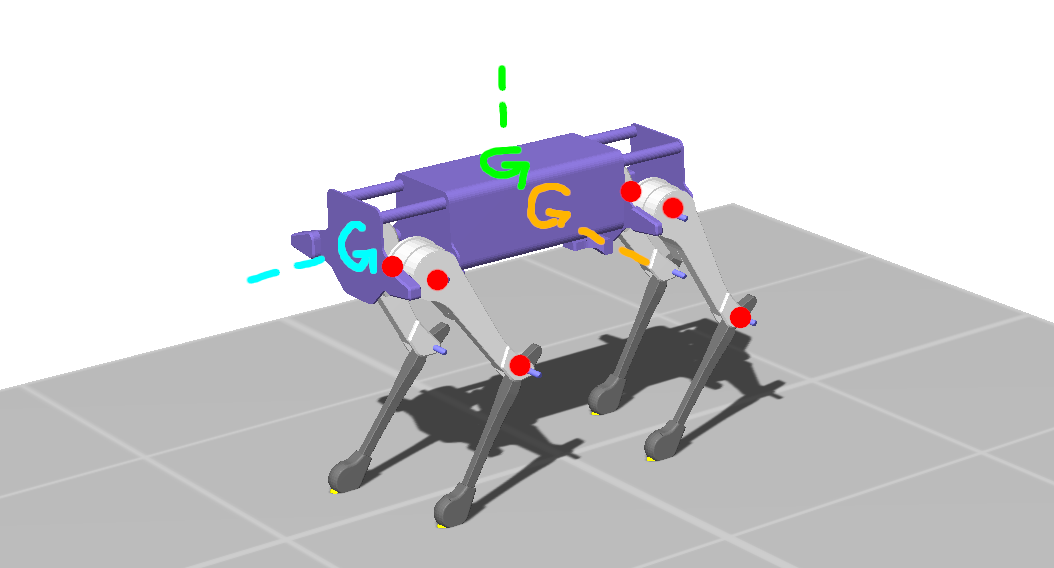
\includegraphics[width=.5\linewidth]{figures/laikago_zoom.png}
    \caption[Quadruped Robot "Laikago"]{Quadruped Robot "Laikago". Red dots denote positions of leg motors on one side. Rotations: green = yaw, orange = pitch, blue = roll.}
    \label{fig:lkg}
    \end{figure}

    In the Drop Test the entire robot was moved a fixed distance up above the ground, rotated about its roll and pitch axes and let fall freely. The goal was to find motor parameters for which the robot would land on its feet without tipping for as large of a roll/pitch rotation as possible. The disturbance space was hence chosen to be spanned by the roll displacement and the pitch displacement, each allowing both positive and negative values. Its boundaries were chosen by visual inspetion as $\pm 0.6$ radians, which were the positive and negative displacements for which the robot was guaranteed to tip over. For the detection of the attractor, a fixed point, the simulation was run for a brief amount of time for the robot to settle into a stable position. When evaluating convergence however, the theory based approach didn't work. Because of the copmliance of the robot, it would bounce slightly and never land in exactly the same position from which it was lifted up in the first place. Because of this the state trajectory would not converge even when the robot landed successfully. To remedy this, convergence was redefined for this test. The goal was after all not for Laikago to land in the exact same spot, but to just land upright on its feet. This was characterized by taking only coordinates of the core of the robot into account. Its height, roll and pitch coordinates were all to be close to the corresponding coordinates in the attractor. Yaw, horizontal translation and the exact position of the legs were disregarded.
    As the time until contact with the gound was quite consistent, the simulation was run for a bit longer and if convergence was not detected within that time it was concluded that the robot had tipped over. This approach of evaluating convergence is far from rigorous, but it worked flawlessly and was both simpler to implement and computationally more effitient than the method derived from theory. 

    \begin{figure}[h!]
    \centering
        \begin{minipage}{0.32\textwidth}
            \centering
            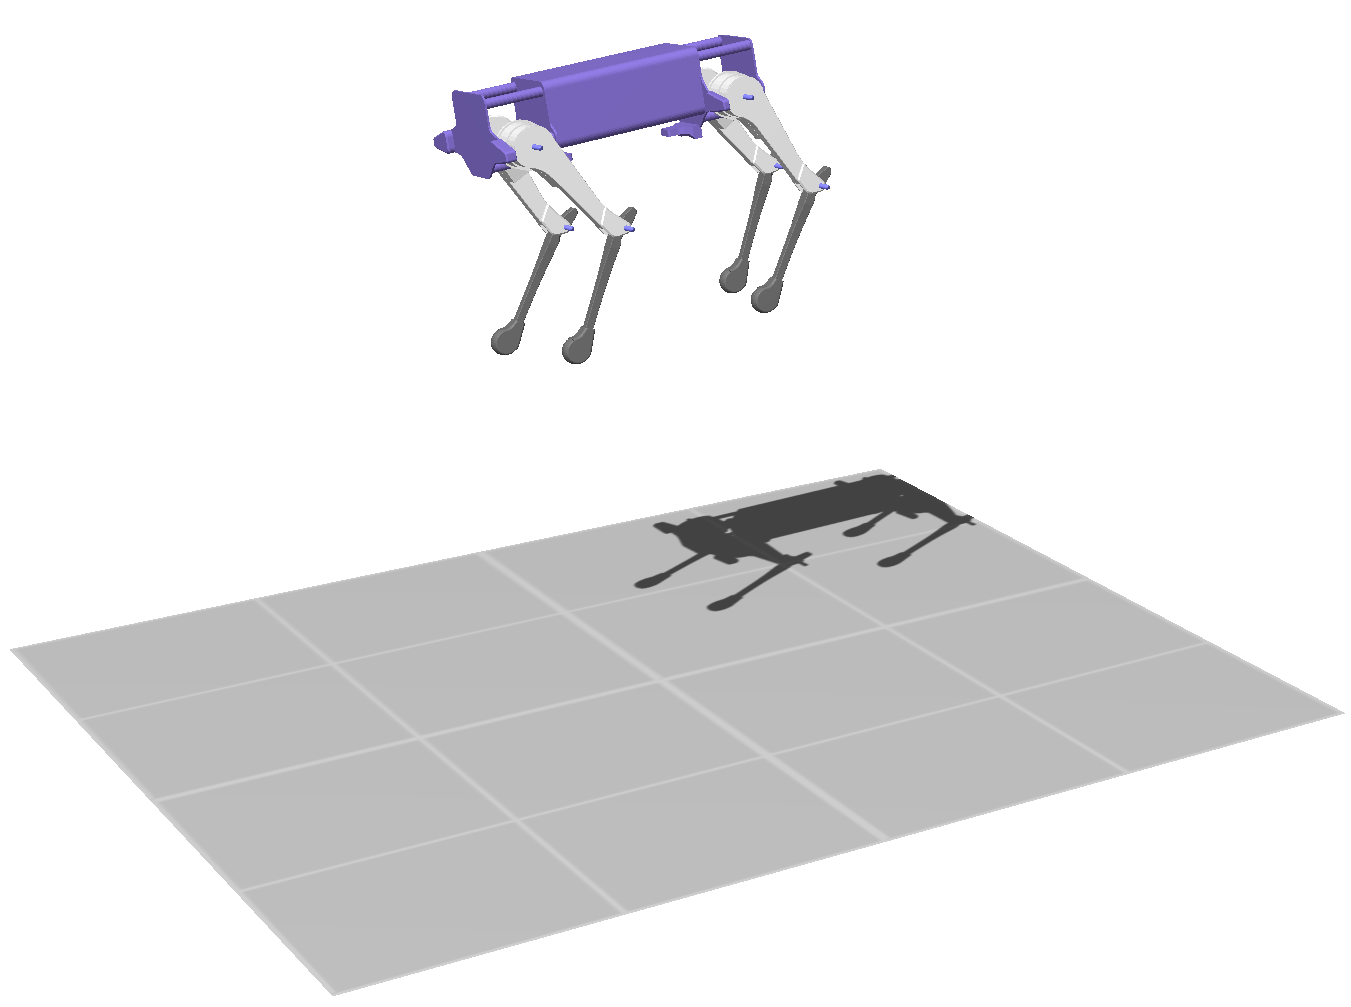
\includegraphics[width=\textwidth]{figures/lkgdrop_1_crop.png} % second figure itself
            %\caption{second figure}
        \end{minipage}
        \begin{minipage}{0.32\textwidth}
            \centering
            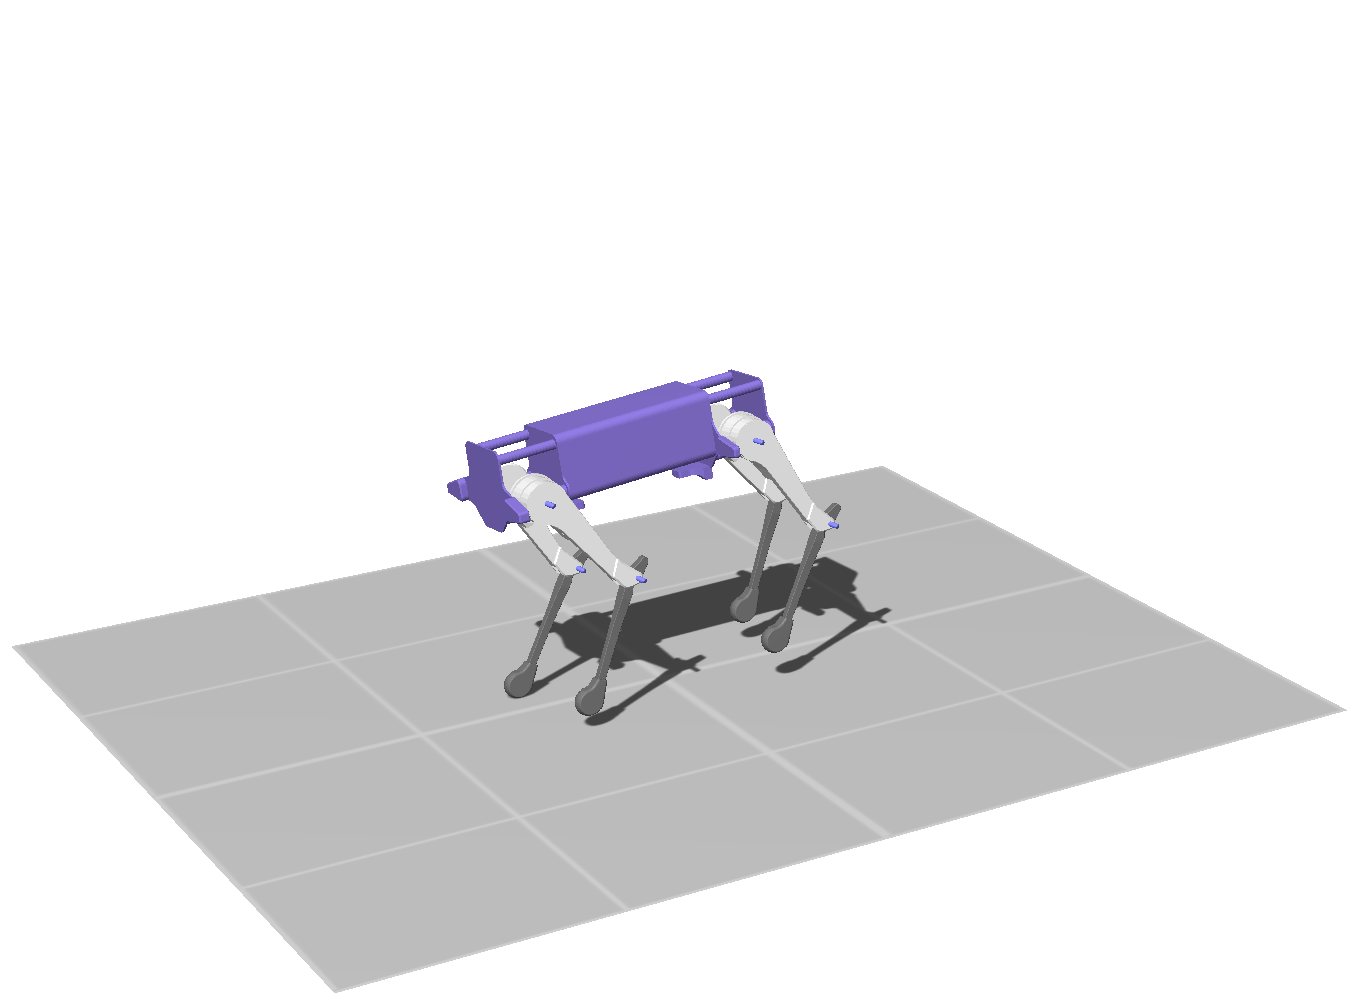
\includegraphics[width=\textwidth]{figures/lkgdrop_2_crop.png} % first figure itself
            %\caption{first figure}
        \end{minipage}
        \begin{minipage}{0.32\textwidth}
            \centering
            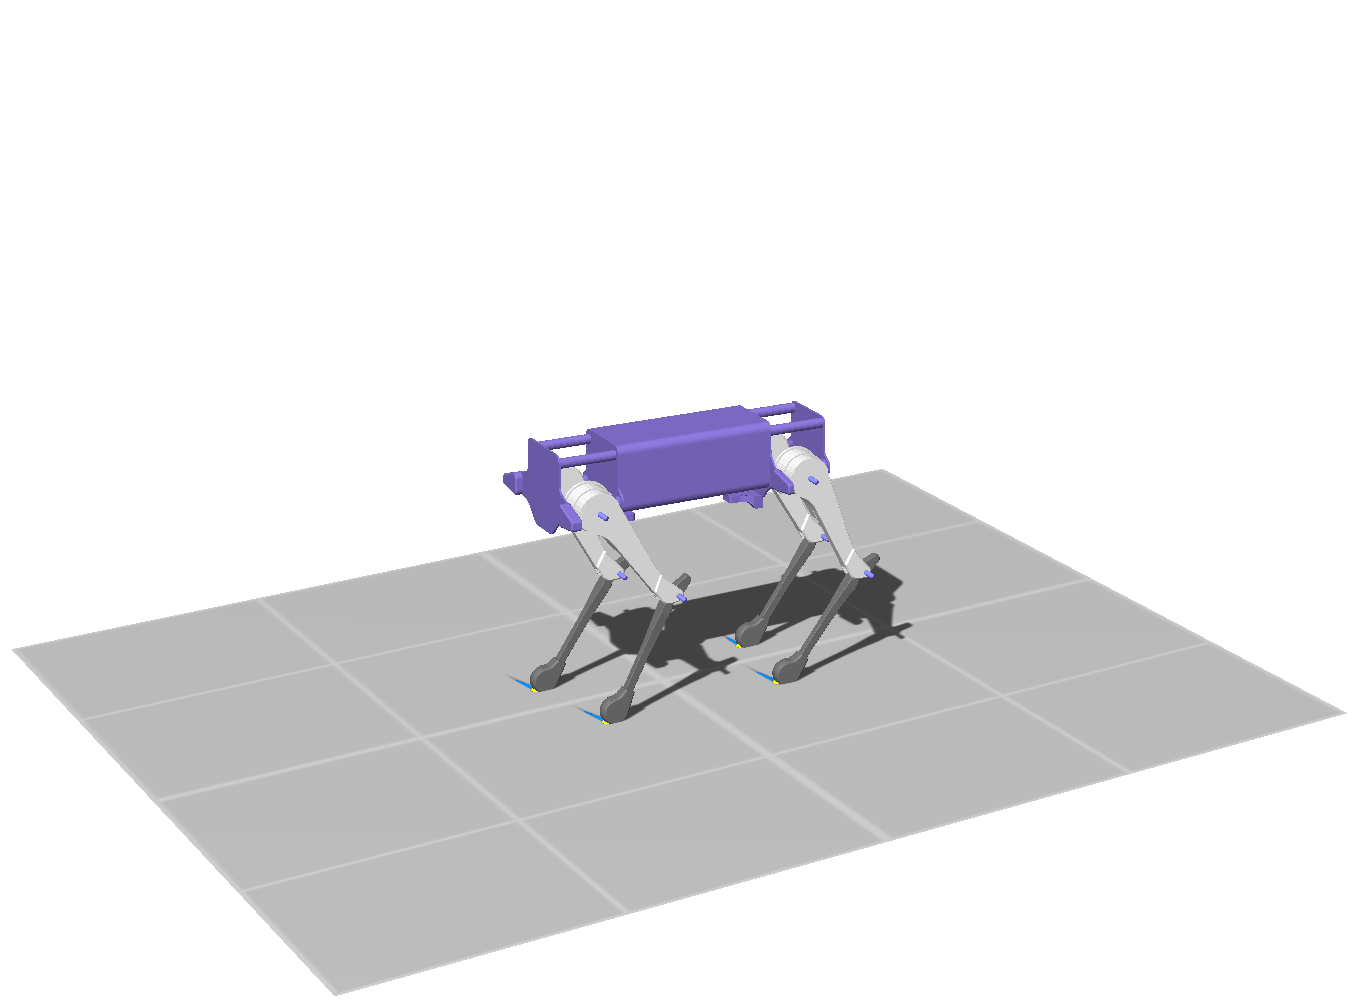
\includegraphics[width=\textwidth]{figures/lkgdrop_3_crop.png} % second figure itself
            %\caption{second figure}
        \end{minipage}
        

    \caption{Drop Test Visualization}
    \label{fig:droplkg}

\end{figure}

    For the Swing Test, the robot was kept in its initial standing pose and disturbances took the form of oscillating the ground back and forth. This means disturbances were now applied continuously and in case of convergence, the state trajectory of the robot would (optimally) never leave the attractor. The disturbance space was chosen as the span of amplitude and frequency of the oscillation. With this choice robustness would be evaluated w.r.t. general oscillations about the roll axis, i.e. both low frequencey and high amplitude and vice versa. As amplitudes and frequencies only make sense for positive values, the disturbance space was only analyzed in the first quadrant of the two dimensional plane. The upper boundary of $0.3$ radians for the amplitude was chosen to be slightly higher than the value for which the robot would start to tip over when the ground wasn't moving. The frequencies were limited to 5 Hz after visual inspection. 
    The attractor coincided with the previous test, as with zero disturbance it would take its standing pose. 
    Again the convergence evaluation proved problematic, as the state trajectory would only be on the attractor for brief periods of time while oscillatiog back and forth. To remedy this, the states were tranesformed s.t. they were expressed in the coordinate frame of the ground itself. With this convergence should have been possible to be evaluated, however slight wobbling of the robot cause it to slip on the ground. Here again the convergence definition was loosend and only height, pitch and roll of the core compared to the attractor. As in the first test, this approach proved successfull. 

     \begin{figure}[h!]
    \centering
        \begin{minipage}{0.3\textwidth}
            \centering
            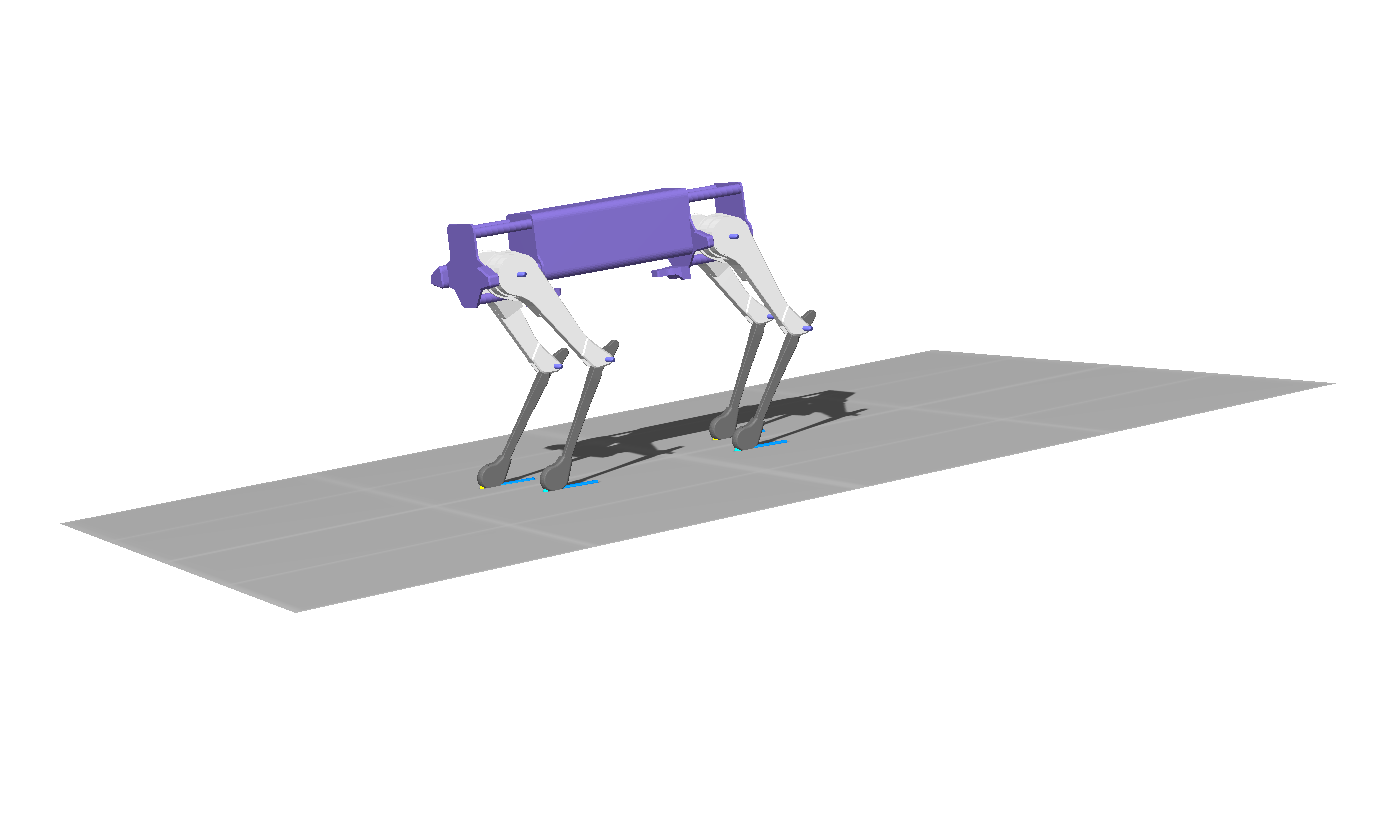
\includegraphics[width=\textwidth]{figures/lkgswing_1_crop.png} % second figure itself
            %\caption{second figure}
        \end{minipage}
        \begin{minipage}{0.3\textwidth}
            \centering
            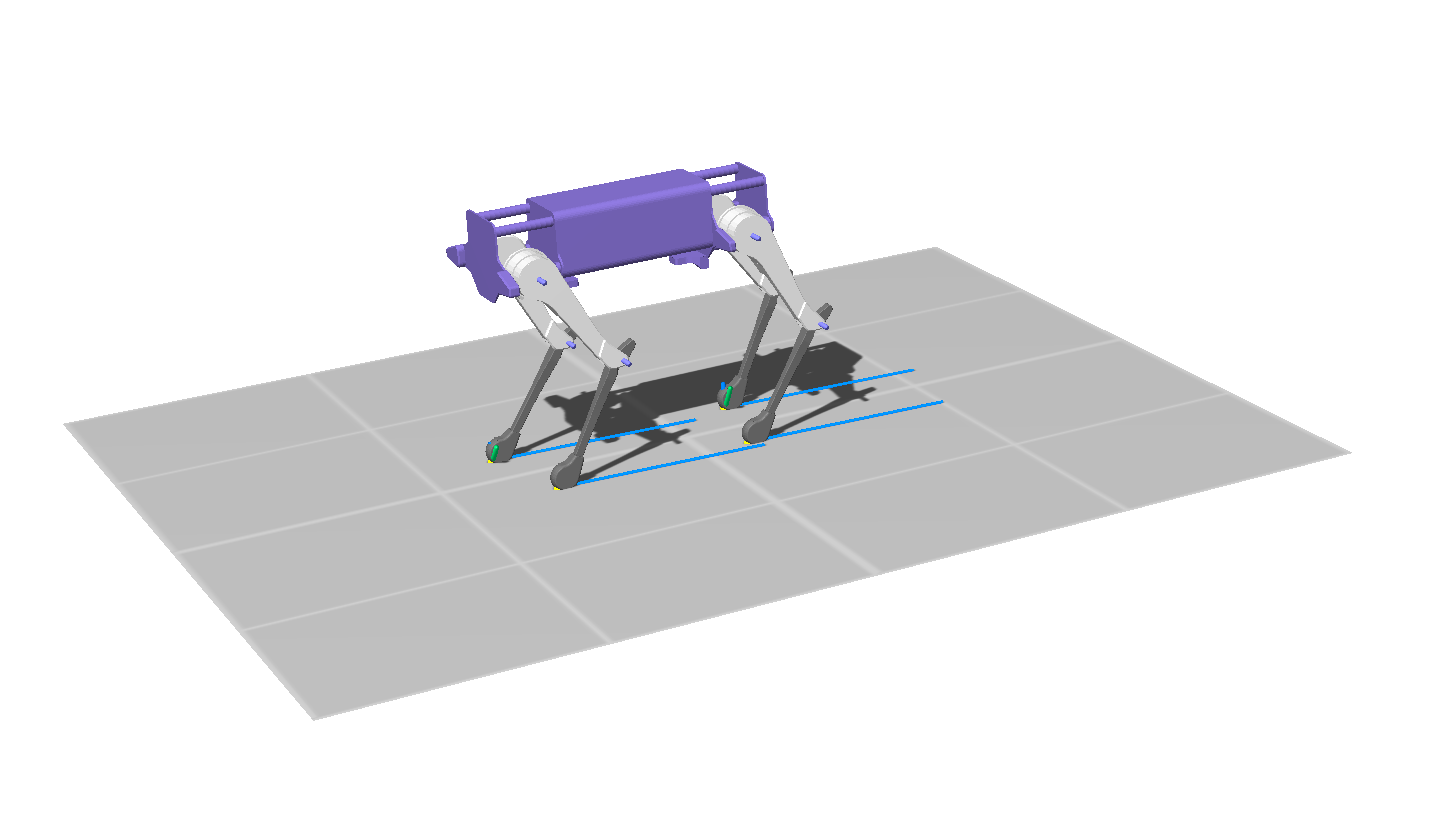
\includegraphics[width=\textwidth]{figures/lkgswing_2_crop.png} % first figure itself
            %\caption{first figure}
        \end{minipage}
        \begin{minipage}{0.3\textwidth}
            \centering
            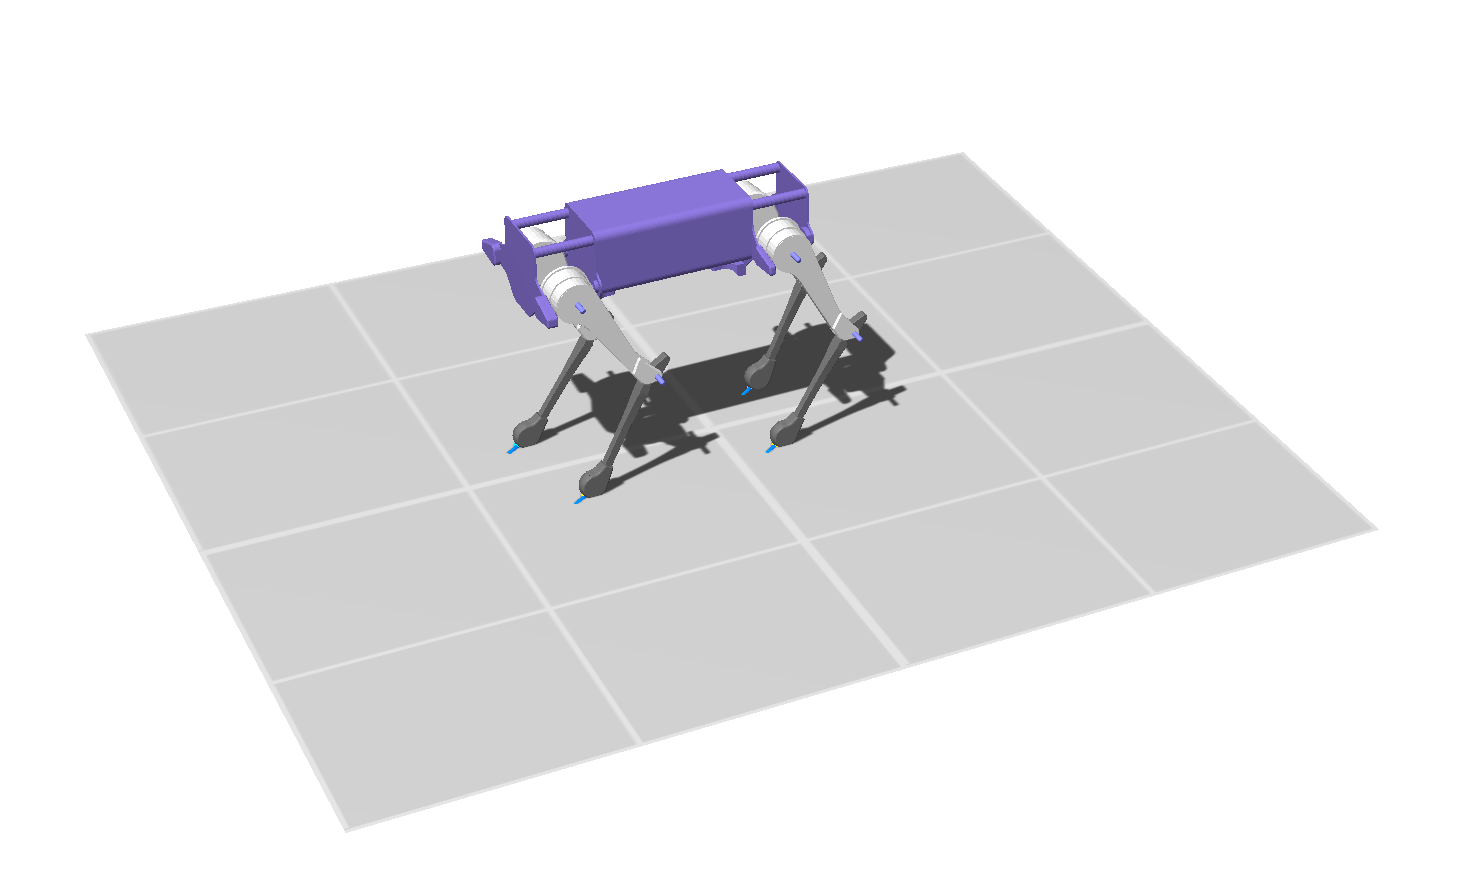
\includegraphics[width=\textwidth]{figures/lkgswing_3_crop.png} % second figure itself
            %\caption{second figure}
        \end{minipage}
        

    \caption{Swing Test Visualization}
    \label{fig:droplkg}
    
\end{figure}


    For both tests, the proper function of the convergence evaluation was verified by visually inspecting final states of trajectories to the determined outome. All the test specific adaptations were implemented in the function handling the simulation and evaluation of trjaectories, represented by the yellow fields in figure \ref{framework}. The application of parameters was specific to Laikago, but identical for both tests. The rest of the framwork remained untouched.
    %For both tests the setting of parameters stayed the same, however the application of disturbances and .. see yellow things in framework.








    %The choice of disturbance space was limited to 2 dimensions for ease of visualization and analysis.  
    
    %The first of these is the function applying the parameters to the system. This is generally as simple as changing some variables but fully depends on and needs to be customized for the specific system at hand.  

    %The second is arguably the more essential one. This is the function called by the multithreading pipeline. It needs to run the simulation, apply disturbances, whether continuously or only initially, and evaluate the convergence, returning the boolean result. Concrete examples are listed in the TESTs section. 

    %how the two functions worked for individual laikago tests, highlighting simplifications from the rigorous definitions layed out before
    
    %go into detail on laikago testing setup. 
    
    %analysis needed to find parameter space and disturbance space boundaries and good initial guesses.
    %analysis of high dof motion tricky (bad 3d image), rather plot every coordinate over time (image). 

    %Laikago implementation of test. 
    %applyParameters
        %very much dependent on the particular system and 
    %simAndEval

    %In testing, when applying disturbances to the standing quadruped, "convergence to the attractor" really just means the quadruped not tipping over. For this there doesn't just exist one single valid state as any translation along the horizontal plane or rotations about the vertical axis leave the robot still standing upright. In these cases it is simpler to actively check whether the system diverges, i.e. tips over, as it already starts on the attractor and one intuitively knows that it won't stand up by itself and can therefore not return after leaving it. In this specific case this also meant that once "tipping over" was detected, the individual simulation was stopped.  Divergence was detected by verifying that the hight of the core of the robot was suffitiently high above the ground and both pitch and roll didn't deviate much from the original position. We do still compute an attractor, however only choose the three relevant coordinates of the core for future states to be compared to. (maybe put this part to the results?)

    

\chapter{Results} \label {results}
    
    The computation of the following results was carried out on a 64 bit computer, with an Intel i7 processor consisting of 8 1.8 GHz cores. 
    First the proper function of the robustness measure computation was verified before making attempts of optimizing the system parameters.   

    %Initially, simple systems were analyzed to gain familiarity with dde and it's implementation. Visualizing 3d time dependent trajectories all in one plot becomes very convoluted quickly as can be seen in Fig .. . This is especially true when working with multibody systems. Attempts were made to apply principle component analysis to reduce the dimensionality, however this only yielded usable data when working with multibody systems where all bodies moved in a coordinated fashion. In these cases picking out and tracking individual bodies yielded


    %Another issue is that for effitient computation, yada yada let's see how much we want to talk about PCA anyways.  
    \iffalse
    It is much more practical to plot the evolution of individual coordinates over time, as trends are much more evident and 

    "While visually appealing, these graphs were less useful for actual inspection of the trajectories."

    Initial familiarization with data.
        plot coordinates over time individually and maybe more importantly, in 2d plots. Compare to convoluted 3d attempts. 
        maybe failed approaches with pca. better to just track less coordinates

    \fi
    
    \subsection{minRad efficiency}


    \begin{figure}[hb!]
    \centering
    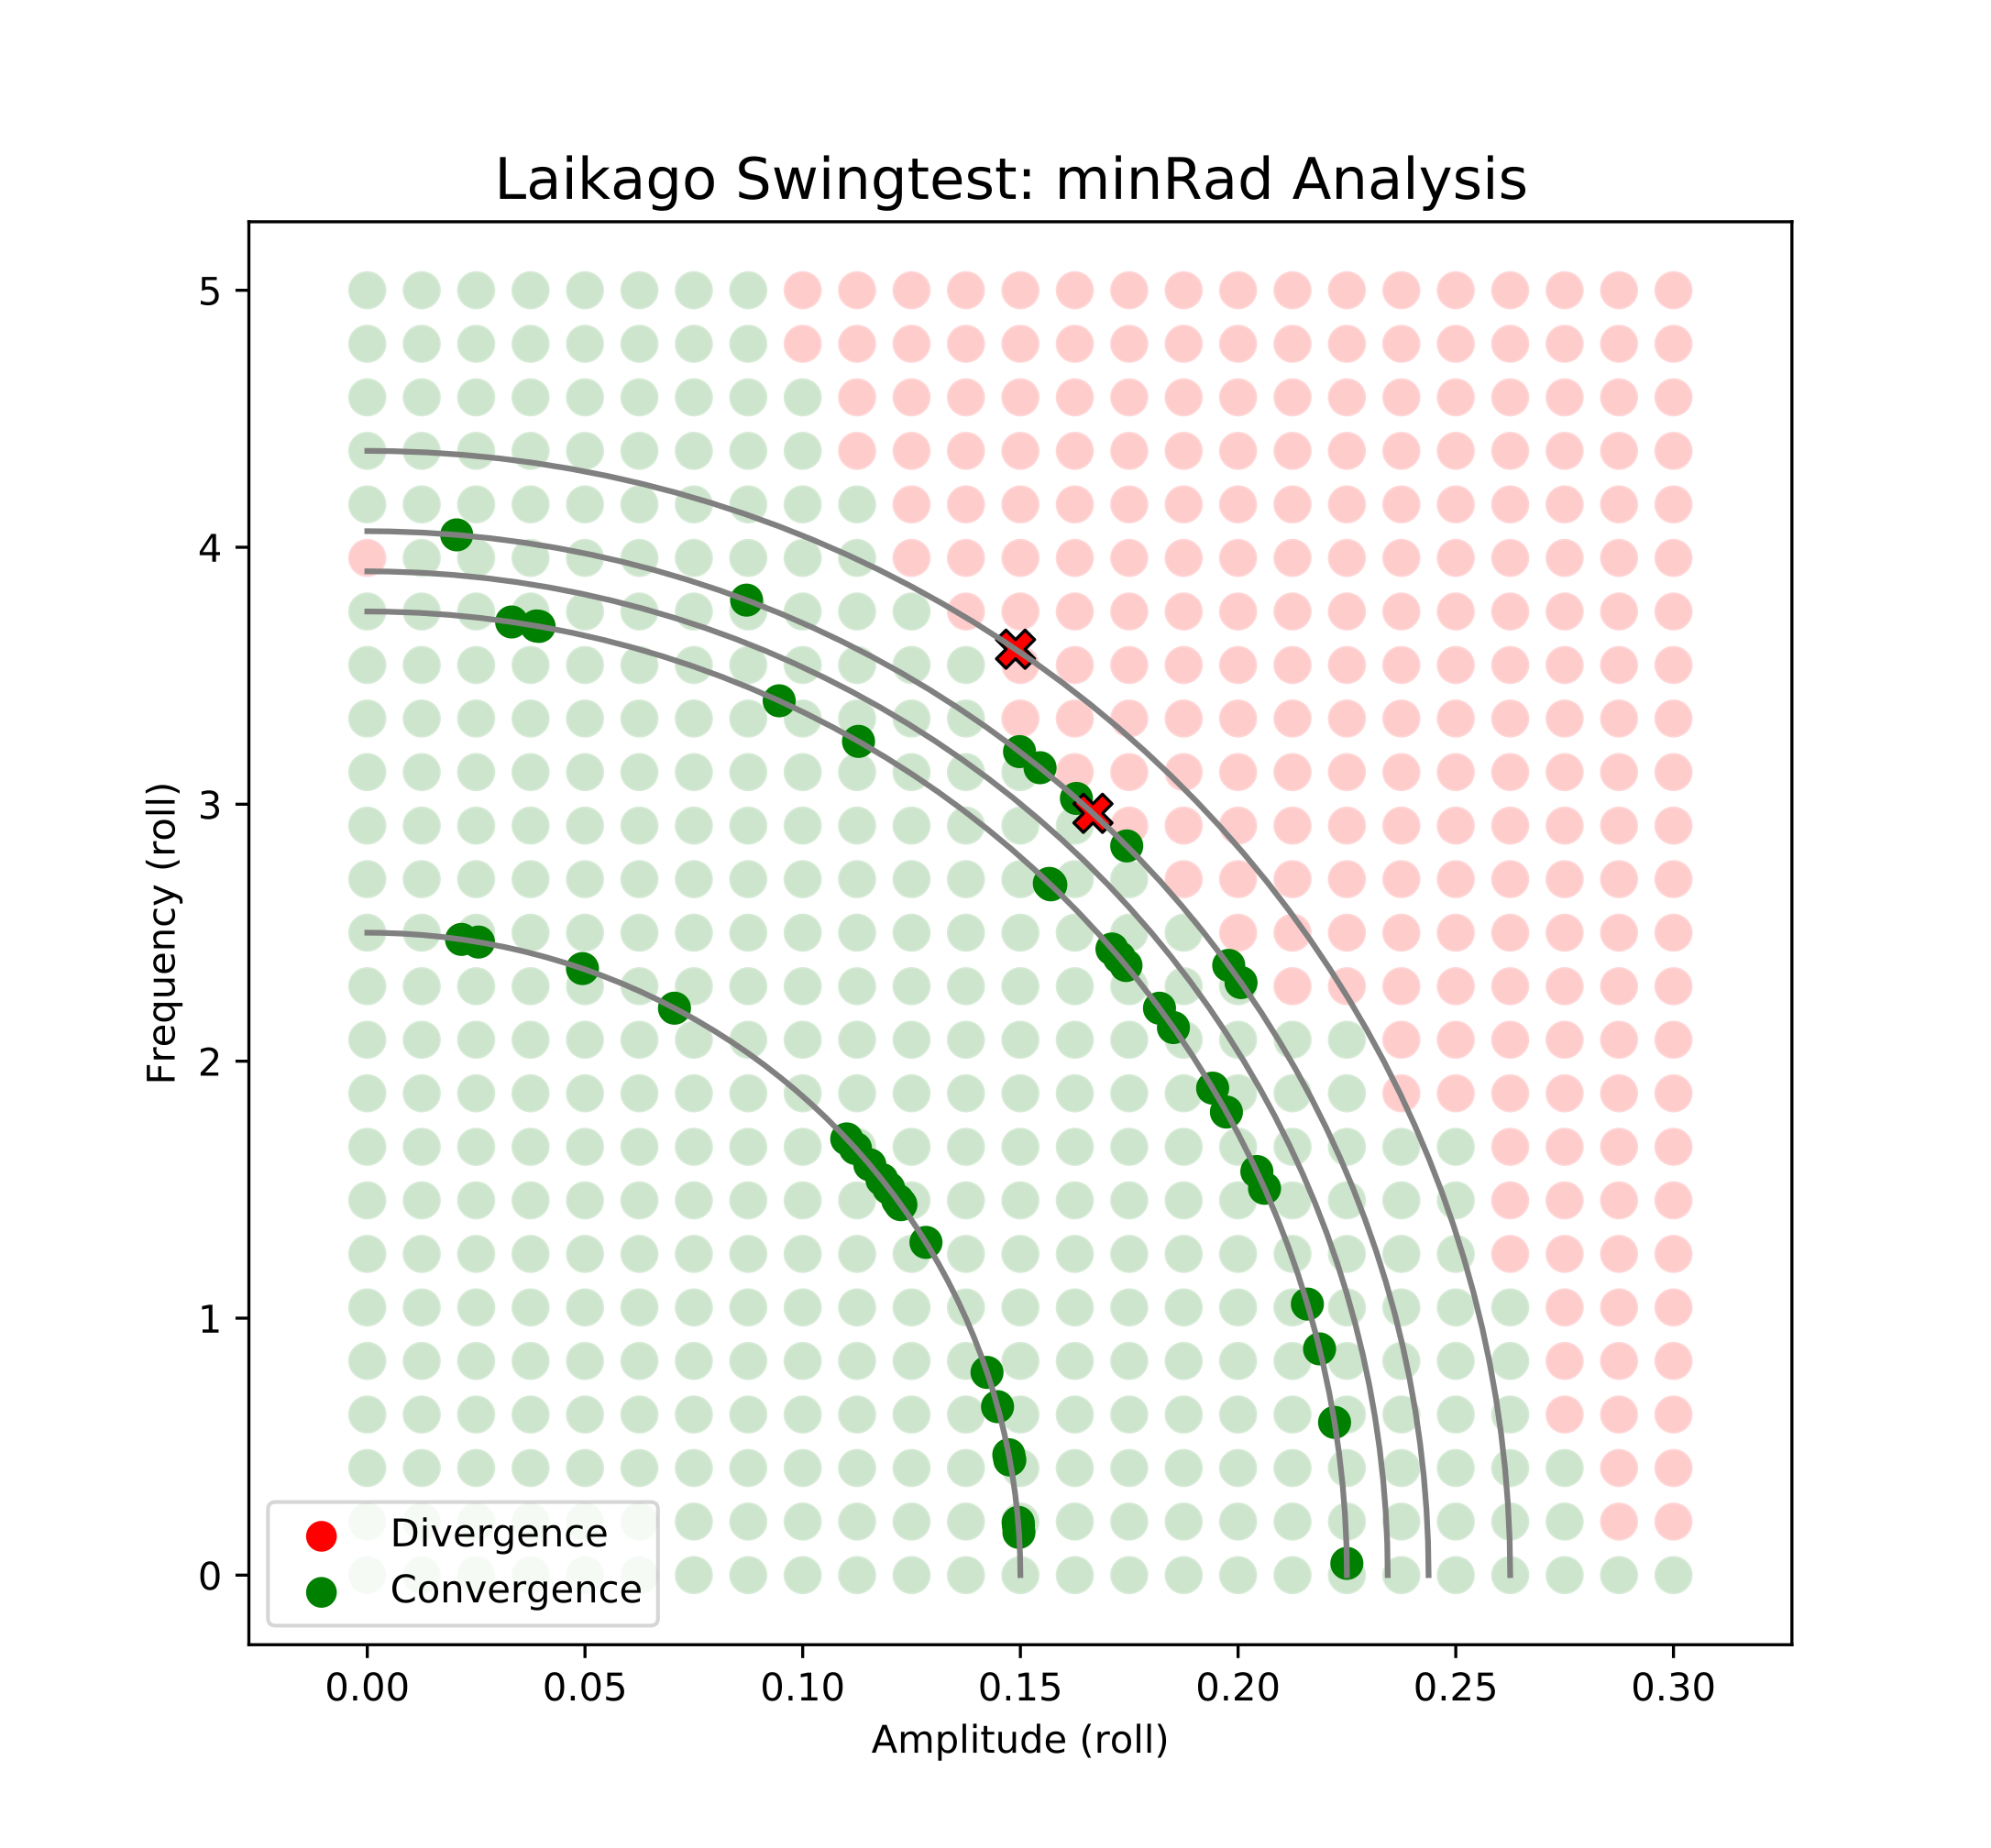
\includegraphics[width=.5\linewidth]{figures/minrad_analysis_v2.png}
    \caption[minRad Result Analysis]{Overlay of results from minRad algorithm and discretization approach, for identical system and parameters. Each gray quarter circle represents one iteration of the minRad algorithm. The final guess for the minimal radius is the radius of the second outermost circle. The same accuracy is achieved using significantly fewer samples when compared to the discretization.}
    \label{fig:minradanal}
    \end{figure}
    The efficiency of the minRad algorithm was measured in an exemplary fashion by comparing it to the results of measuring the minimal radius in a discretized disturbance space. The discretization was chosen to have a step size $h =\frac{1}{25}$ of the domain along each dimension. To achieve a comparable accuracy, $n_{i} = \log_{0.5}(\frac{1}{25}) \approx 5$ iterations of the minRad algorithm were required. Following figure \ref{fig:minradcomp}, $n_s = 20$ samples was chosen to yield a suffitient accuracy at 5 iterations. For this computation the minRad algorithm took 56 seconds, which is less than one fifth of 307 seconds it took the discretization approach to perform computations to achieve the same accuracy. Figure \ref{fig:minradanal} shows this comparison directly. 

    
    %Introduction to laikago (probably should do that earlier?) => yes. previous section
    %    high dof
    %    rather long computational time when solving trajectories (compared to simpler systems, duh)
    %    how it's implemented (no walking yet) laikago, that it doesn't do anything but try to keep its limbs in the predefined state.  

    \subsection{Laikago Drop Test}
    \begin{figure}b!]
    \centering
    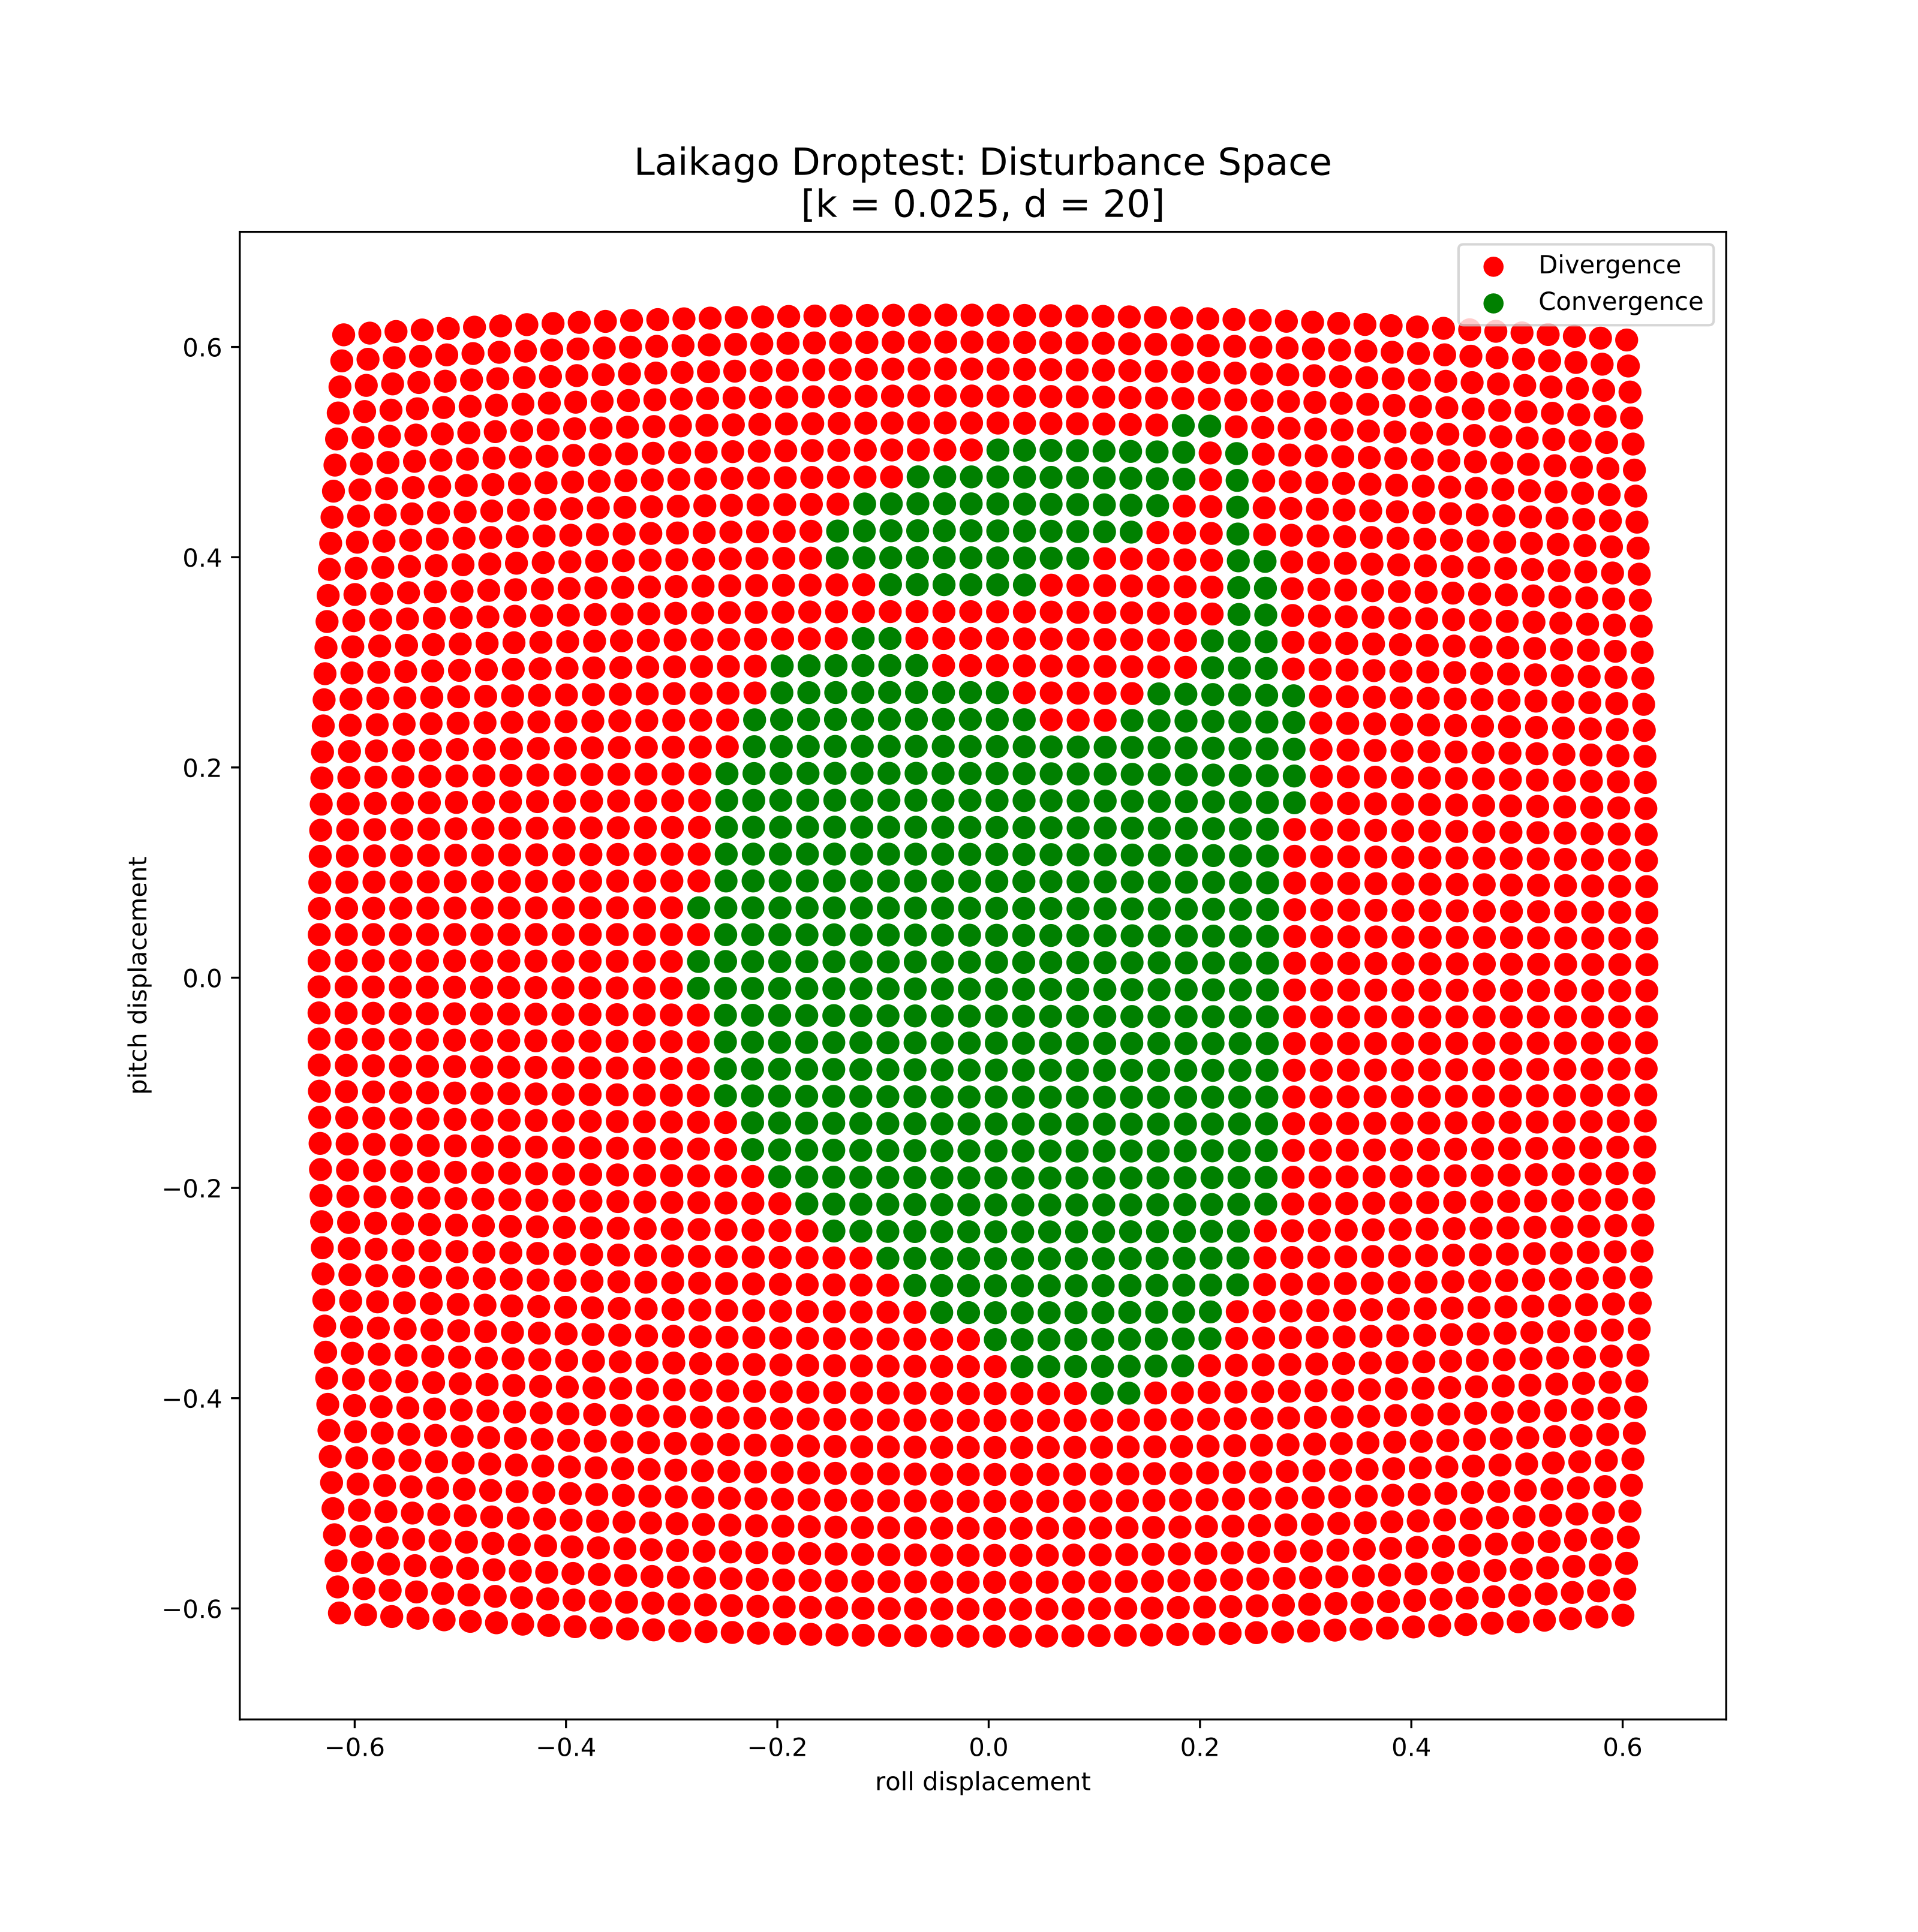
\includegraphics[width=.6\linewidth]{figures/droptest_ds_v2.png}
    \caption[Discretized Disturbande Space, Drop Test]{Discretized disturbance space of the drop test. The color of each point represents whether the robot will land on its feet within a given time frame. The location of each point quantifies the magnitude of the applied disturbance, i.e. a combination of roll and pitch displacement. The irregular shape stems from the pose of the robot not being symmetric.}
    \label{fig:drop}
    \end{figure}    
    In initial tests an arbitrary set of parameters was chosen to inspect the consistency of the minRad algorithm. In figure \ref{fig:drop} the results of evaluating the discretized disturbance space can be seen, showing a connected set of convergence with a relatively smooth boundary. The top region has a part that is almost separated, exemplifying the complex shapes these sets can take. Symmetry about the pitch axis is not given as the pose of the robot is not perfectly symmetric either. One may also notice that the discretization is slightly cuved. This is presumably due to the method of manipulating the robot model. Its coordinates were not set directly, but rather the whole robot was forced into the specified position and orientation by a spring dampener element in the running simulation. As the time alotted for the model to settle into the desired pose was constant for all disturbance samples, the ones farther from the origin presumably didn't have quite enough time to settle, distorting the resulting space.
    
    For confimation of these results a run of the minRad algorithm was performed using the same set of system parameters. The disturbance samples from this can be seen in a direct comparison to the discretized disturbance space in figure \ref{fig:dropoverlay}. The circular arrengement of the samples corresponds to the individual guesses for the minimal radius and their distance from each other reflects the increasingly small adjustment steps taken by the algorithm. The indentation in the set of converging disturbances is confirmed as the algorithm also detects disturbances leading to divergence at that point, indicated by red crosses. Notice also that a minimal amount of diverging disturbances is computed, as the algorithm iterates whenever it encounters one. From this one can confirm that the minRad algorithm does indeed approximate the minimal radius of the set of convergence $\mathsf{D}_c$. Note that for the following results the simulation time was changed, resulting in smaller sets of convergence. 

    \begin{figure}[ht]
    \centering
    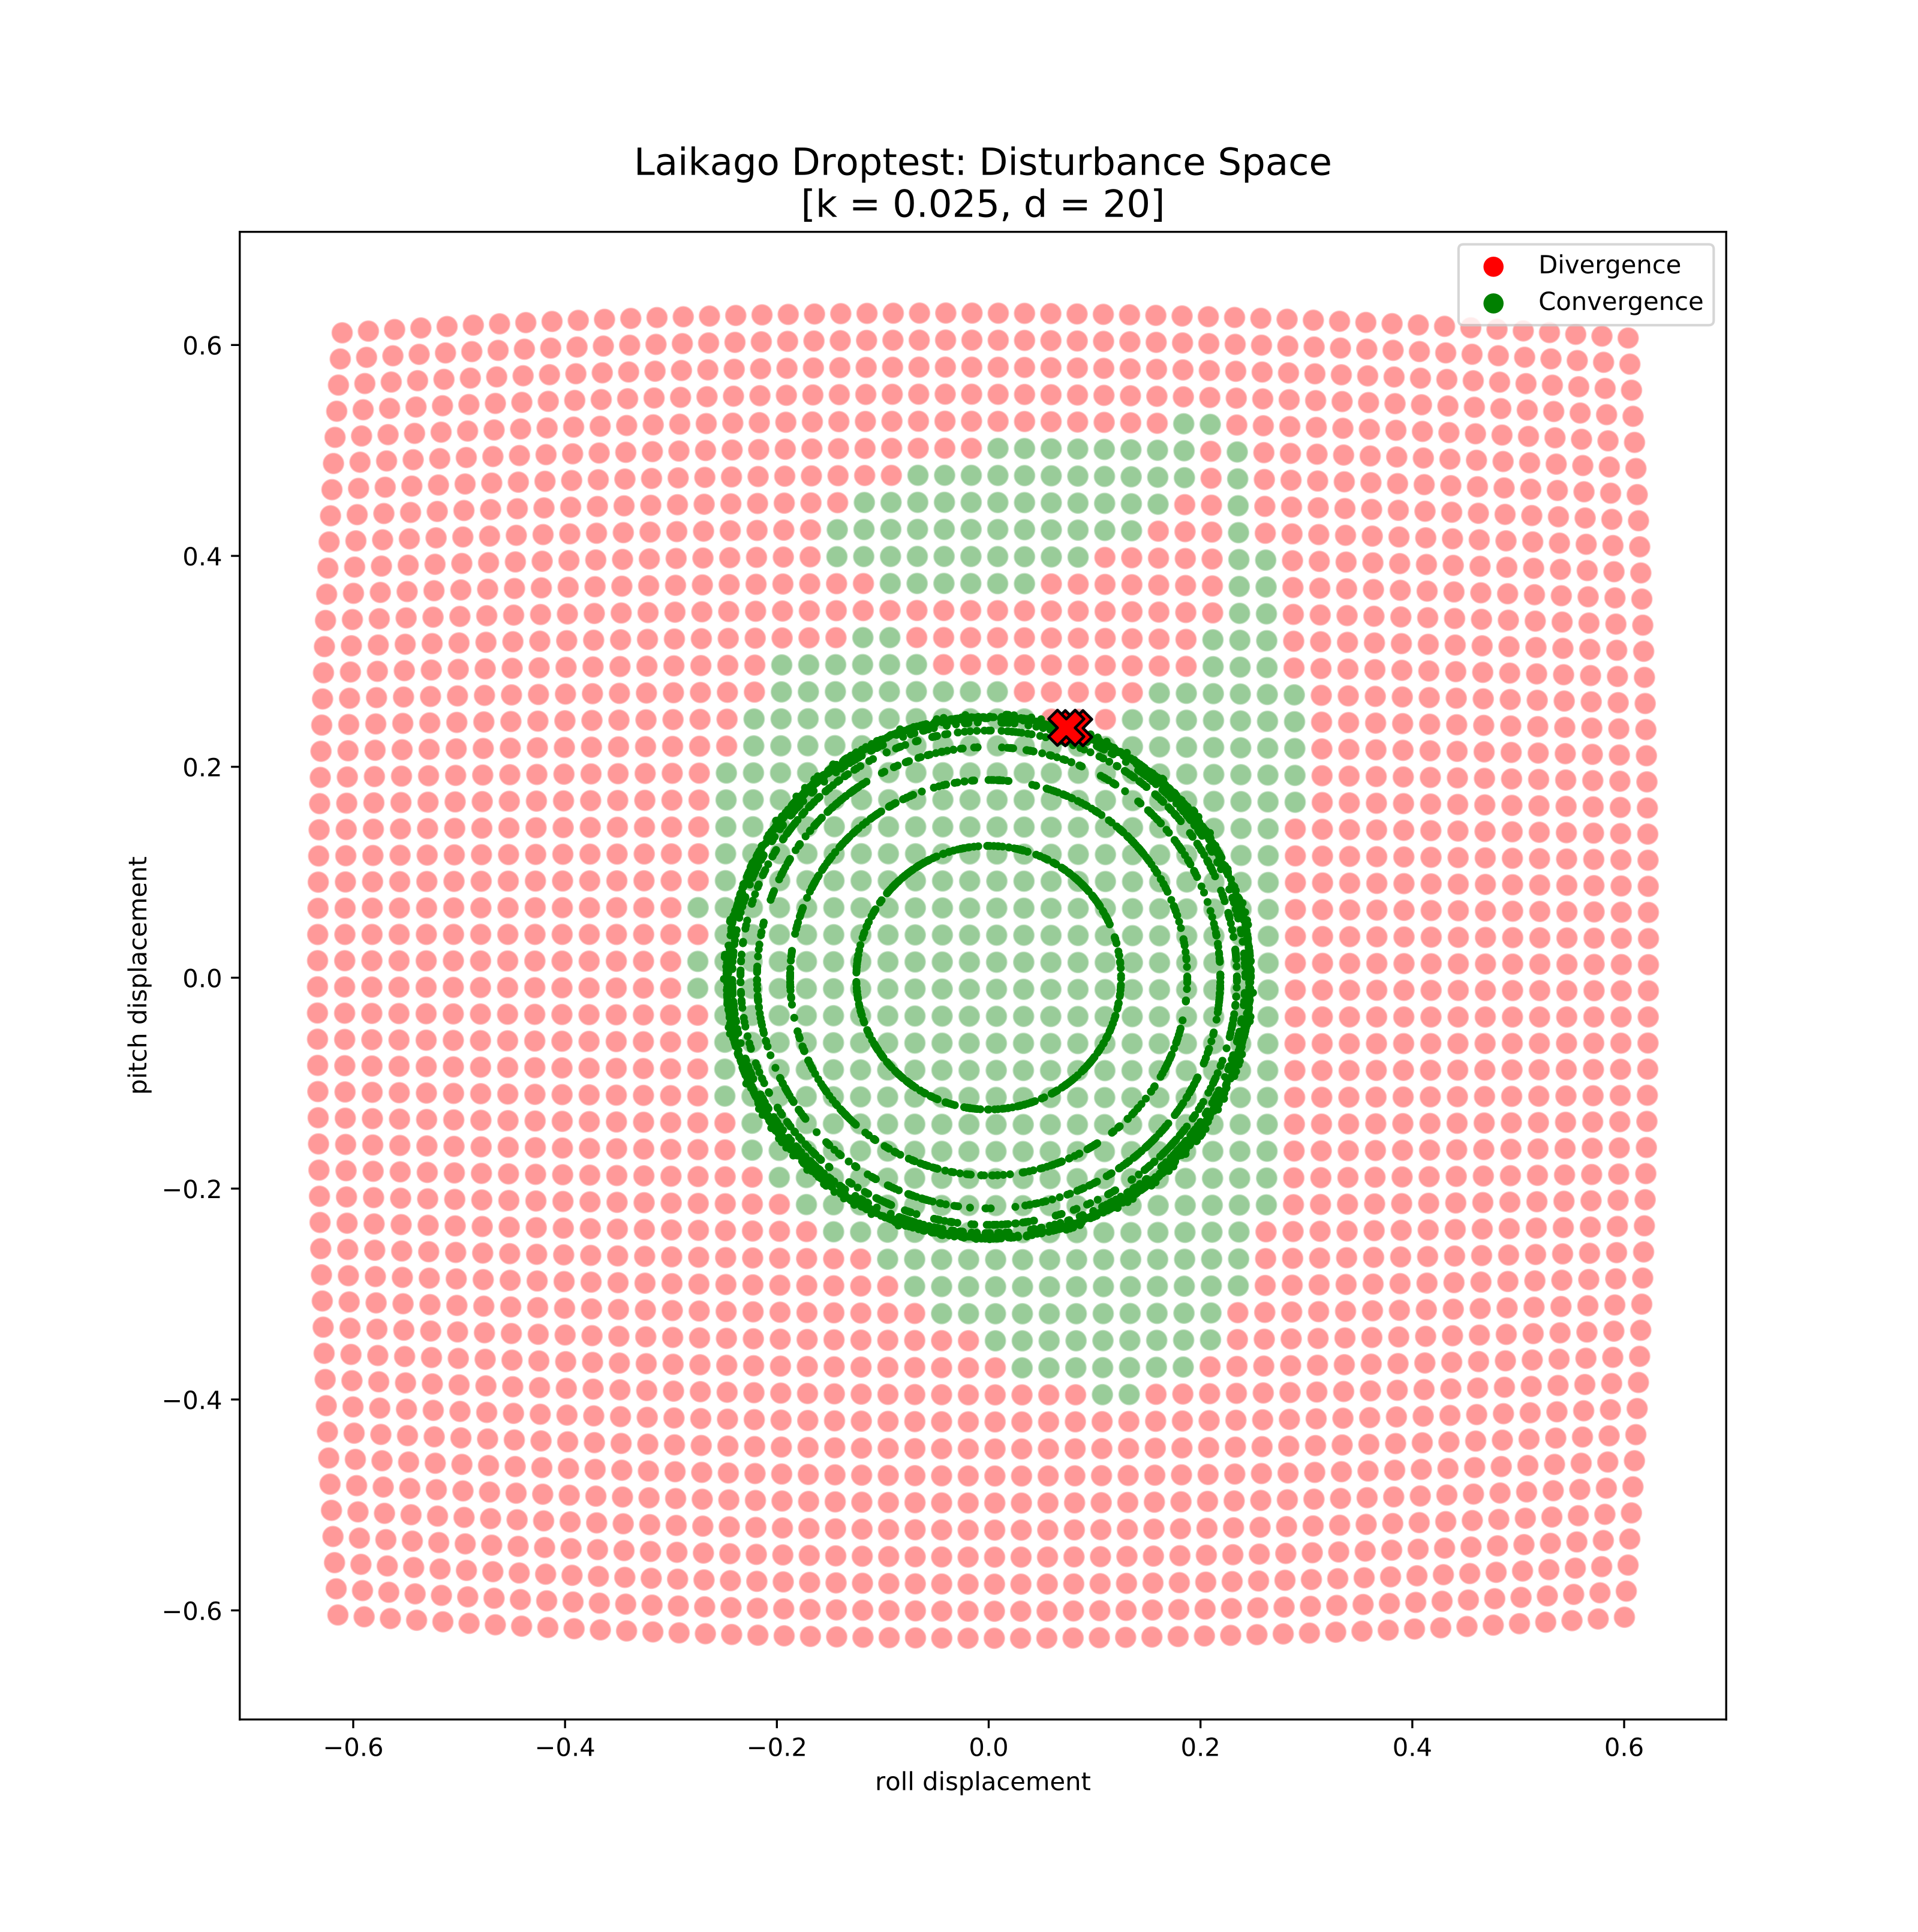
\includegraphics[width=.6\linewidth]{figures/droptest_ds_overay_v10000.png}
    \caption[Overlay of minRad and Discretized Disturbance Space, Drop Test]{Comparison of the samples form the minRad algorithm to those from the discretization. Different radii of circles represent the iteration of the minRad algorithm. It correctly finds the minimal radius at the indentation of the green set.}
    \label{fig:dropoverlay}
    \end{figure}
    \begin{figure}[h]
    %\includegraphics[width=.9\linewidth]{.png}
        \centering
        \begin{minipage}{0.33\textwidth}
            \centering
            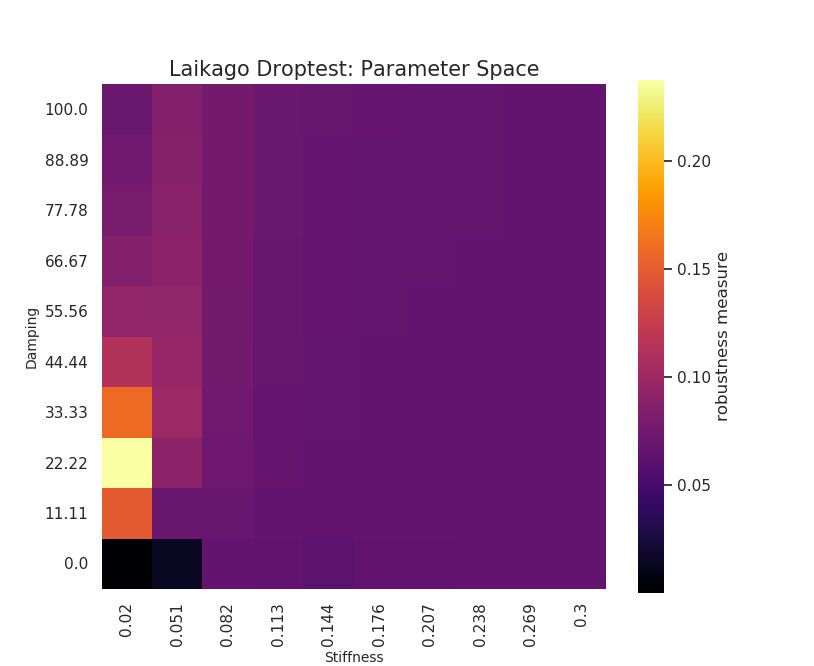
\includegraphics[width=\textwidth]{figures/droptest_ps_full_correct.png} % first figure itself
            %\caption{first figure}
        \end{minipage}\hfill
        \begin{minipage}{0.33\textwidth}
            \centering
            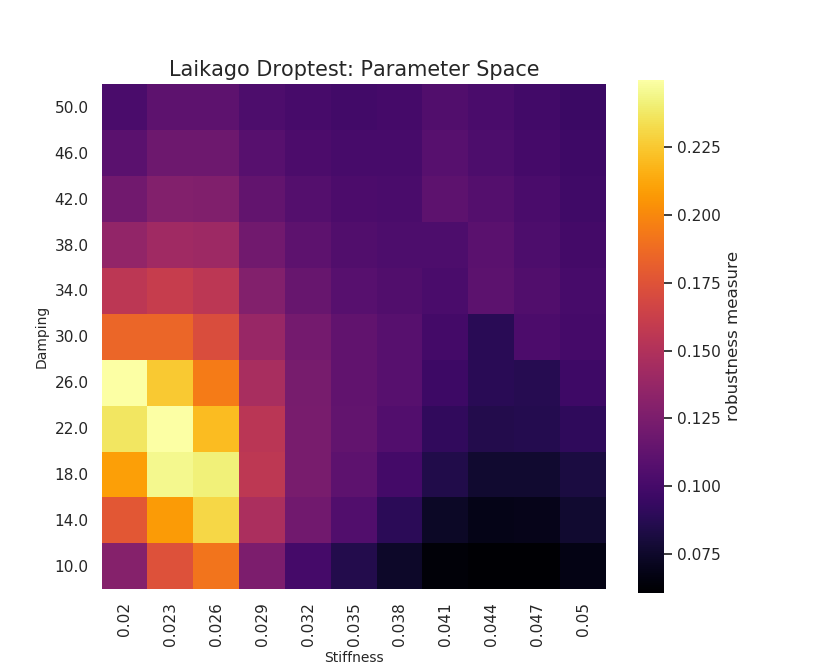
\includegraphics[width=\textwidth]{figures/droptest_ps_zoom1_correct.png} % second figure itself
            %\caption{second figure}
        \end{minipage}
        \begin{minipage}{0.33\textwidth}
            \centering
            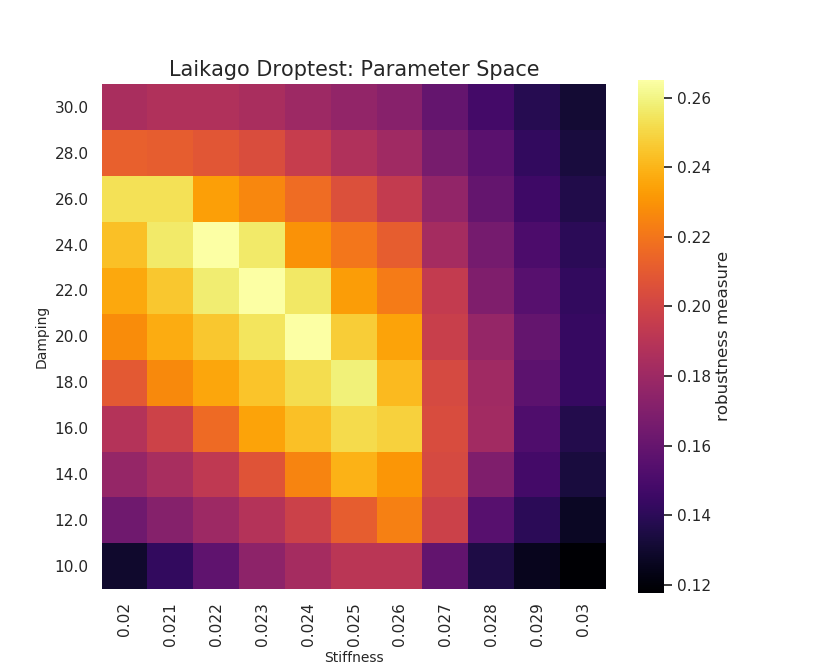
\includegraphics[width=\textwidth]{figures/droptest_ps_zoom2_correct.png} % second figure itself
            %\caption{second figure}
        \end{minipage}

    \caption[Discretized Parameter Space, Drop Test]{Discretized parameter space of the swing test. Lighter colors represent higher robustness for the corresponding parameters. The figures are zoomed in onto the most robust region from left to right.}
    \label{fig:dropps}
    \end{figure}

    With a verified method of computing robustness measures, the parameter space of stiffeness and damping values $\mathsf{P}$ could be explored. The approach for this test was the computation of the robustness measures for all points in the  discretized space. From the results, see figure \ref{fig:dropps}, it was clear that the region of robust parameters was concentrated in one region. Two further computations were performed, each yielding higher resolution of the area of interest, as well as larger optimal robustness values. The time needed for these computations was rather high with over 26 hours each. 

    These results were analyzed by computing discretized disturbance spaces for the optimal set of parameters, as well as a "medium" and a "bad" set with respect to robustness, seen in figure \ref{fig:dropps}. Here one can see that that the bad set of parameters does correspond to the smallest set of convergence, between the optimal and the medium set of parameters however, this is not as clear cut. When counting individual points, the medium result actually has a larger set of convergence, but with respect to the minimal radius they are both equivalent, indicating that higher resolution would be needed for a more detailed disctinction. 

    Visual inspection of the model behaviour confirmed that the optimal parameters did indeed outperform the less robust ones. 



    \begin{figure}[h]
    %\includegraphics[width=.9\linewidth]{.png}
        \centering
        \begin{minipage}{0.33\textwidth}
            \centering
            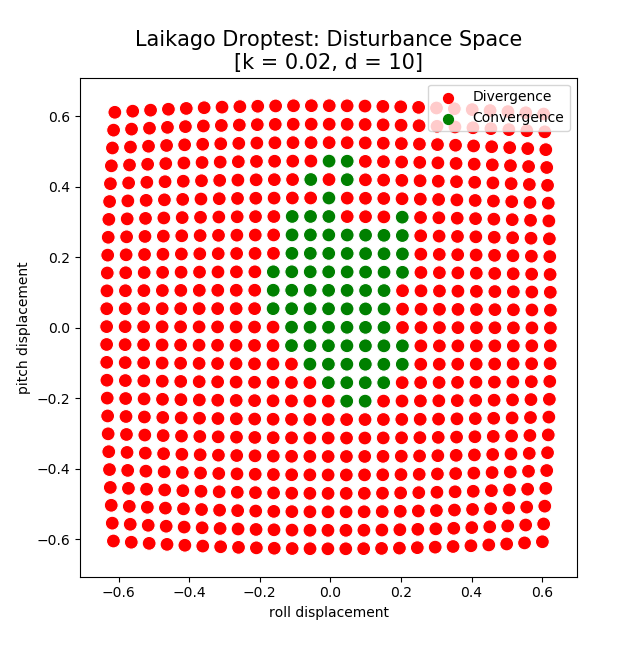
\includegraphics[width=\textwidth]{figures/droptest_ds_bad_correct.png} % first figure itself
            %\caption{first figure}
        \end{minipage}\hfill
        \begin{minipage}{0.33\textwidth}
            \centering
            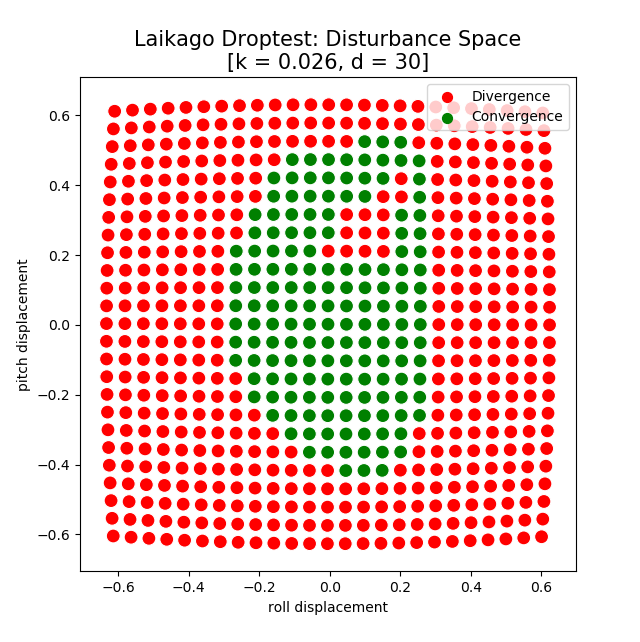
\includegraphics[width=\textwidth]{figures/droptest_ds_medium_correct.png} % second figure itself
            %\caption{second figure}
        \end{minipage}
        \begin{minipage}{0.33\textwidth}
            \centering
            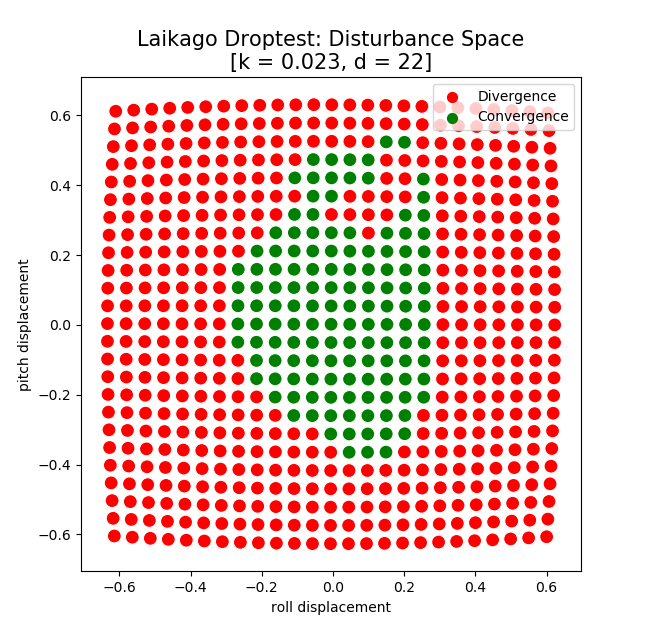
\includegraphics[width=\textwidth]{figures/droptest_ds_opt_correct.png} % second figure itself
            %\caption{second figure}
        \end{minipage}

    \caption[Disturbance Spaces for Selected Parameter Sets, Drop Test]{Disturbance spaces for specific parameters k and d chosen from the discretized parameter space. The corresponding robustness measure increases from left to right. The green area of the rightmost figure is smaller than the middle one, but their minimal radii are approximately equal at this resolution.}
    \label{fig:dropds}
    \end{figure}
    \newpage



    \subsection{Laikago Swing Test}

    The procedure here was analogous to the previous test. First proper function of the minRad algorithm was verified by comparing it to a discretized disturbance space, seen in figure \ref{fig:swingoverlay}. There are two annomalies of convergence in the othervise diverging region, which are attributed to numerical errors but the exact cause couldn't be determined. With that the parameter space was explored, see figure \ref{fig:swingps}, showing a noticably different overall appearance compared to the previouse test. Here the stiffness parameter seems to be the dominant factor regarding robustness, while the damping is less important. The robustness measures are also a lot larger than in the drop test, however this is a direct result from the choice of boundaries on $\mathsf{D}$ and is not a quantitative result.   
    \begin{figure}[h]\label{fig:swingoverlay}
    \centering
    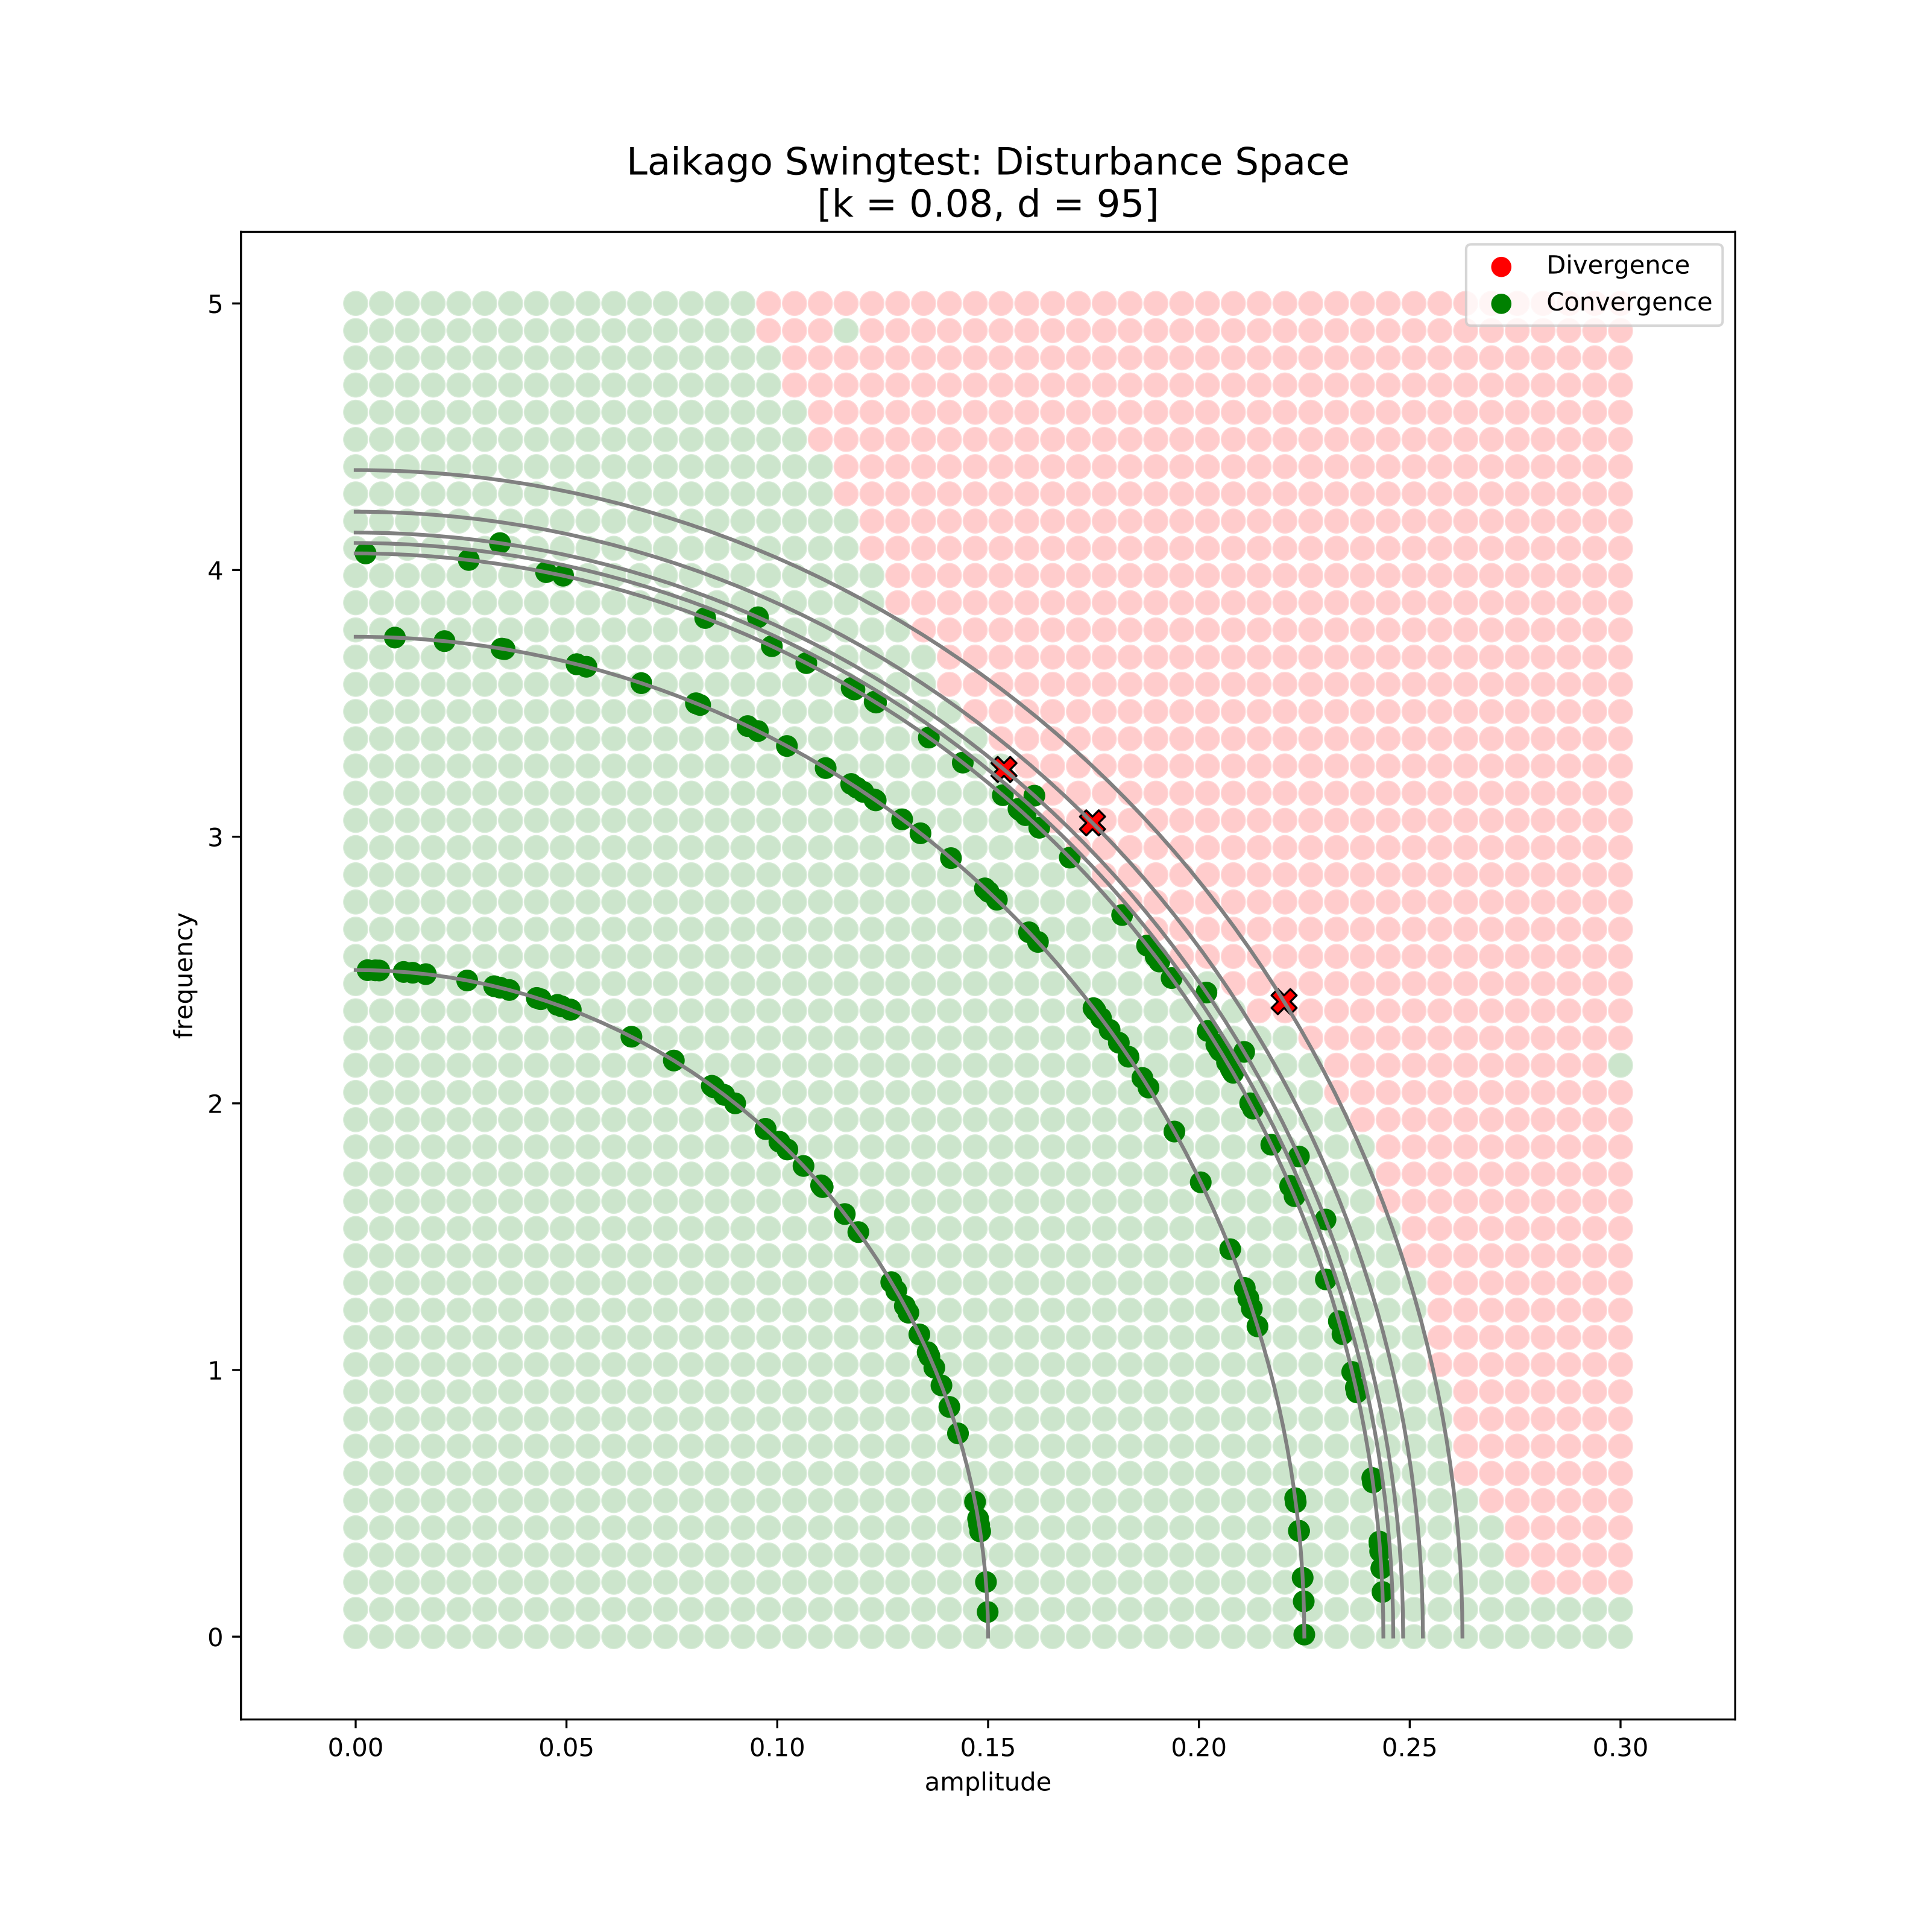
\includegraphics[width=.6\linewidth]{figures/swingtest_ds_overay_v3.png}
    \caption[Overlay of minRad and Discretized Disturbance Space, Swing Test]{Comparison of the samples from the minRad algorithm to those from the discretization. Different radii of circles represent the iteration of the minRad algorithm. Two unexplained annomalies of green dots in an otherwise red area can be seen.}
    \end{figure}    

    \begin{figure}[h]
    \centering
    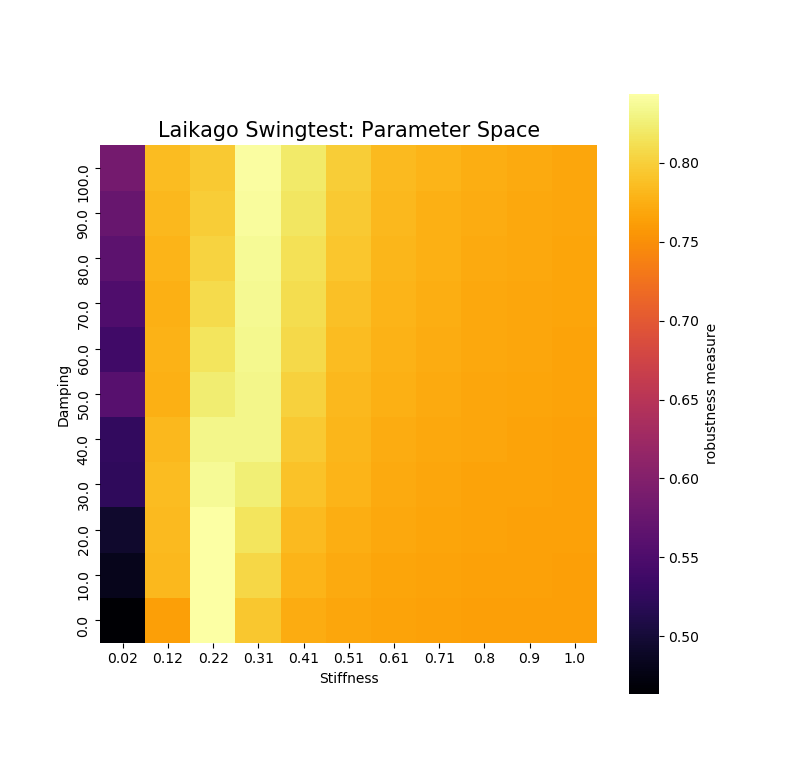
\includegraphics[width=.6\linewidth]{figures/swingtest_ps.png}
    \caption[Discretized Parameter Space, Swing Test]{Discretized parameter space of the drop test. Lighter colors represent higher robustness for the corresponding parameters. A dominant dependence of the robustness measure on the motor stiffness is apparent.}
    \label{fig:swingps}
    \end{figure}    

    \begin{figure}[h]
    %\includegraphics[width=.9\linewidth]{.png}
        \centering
        \begin{minipage}{0.33\textwidth}
            \centering
            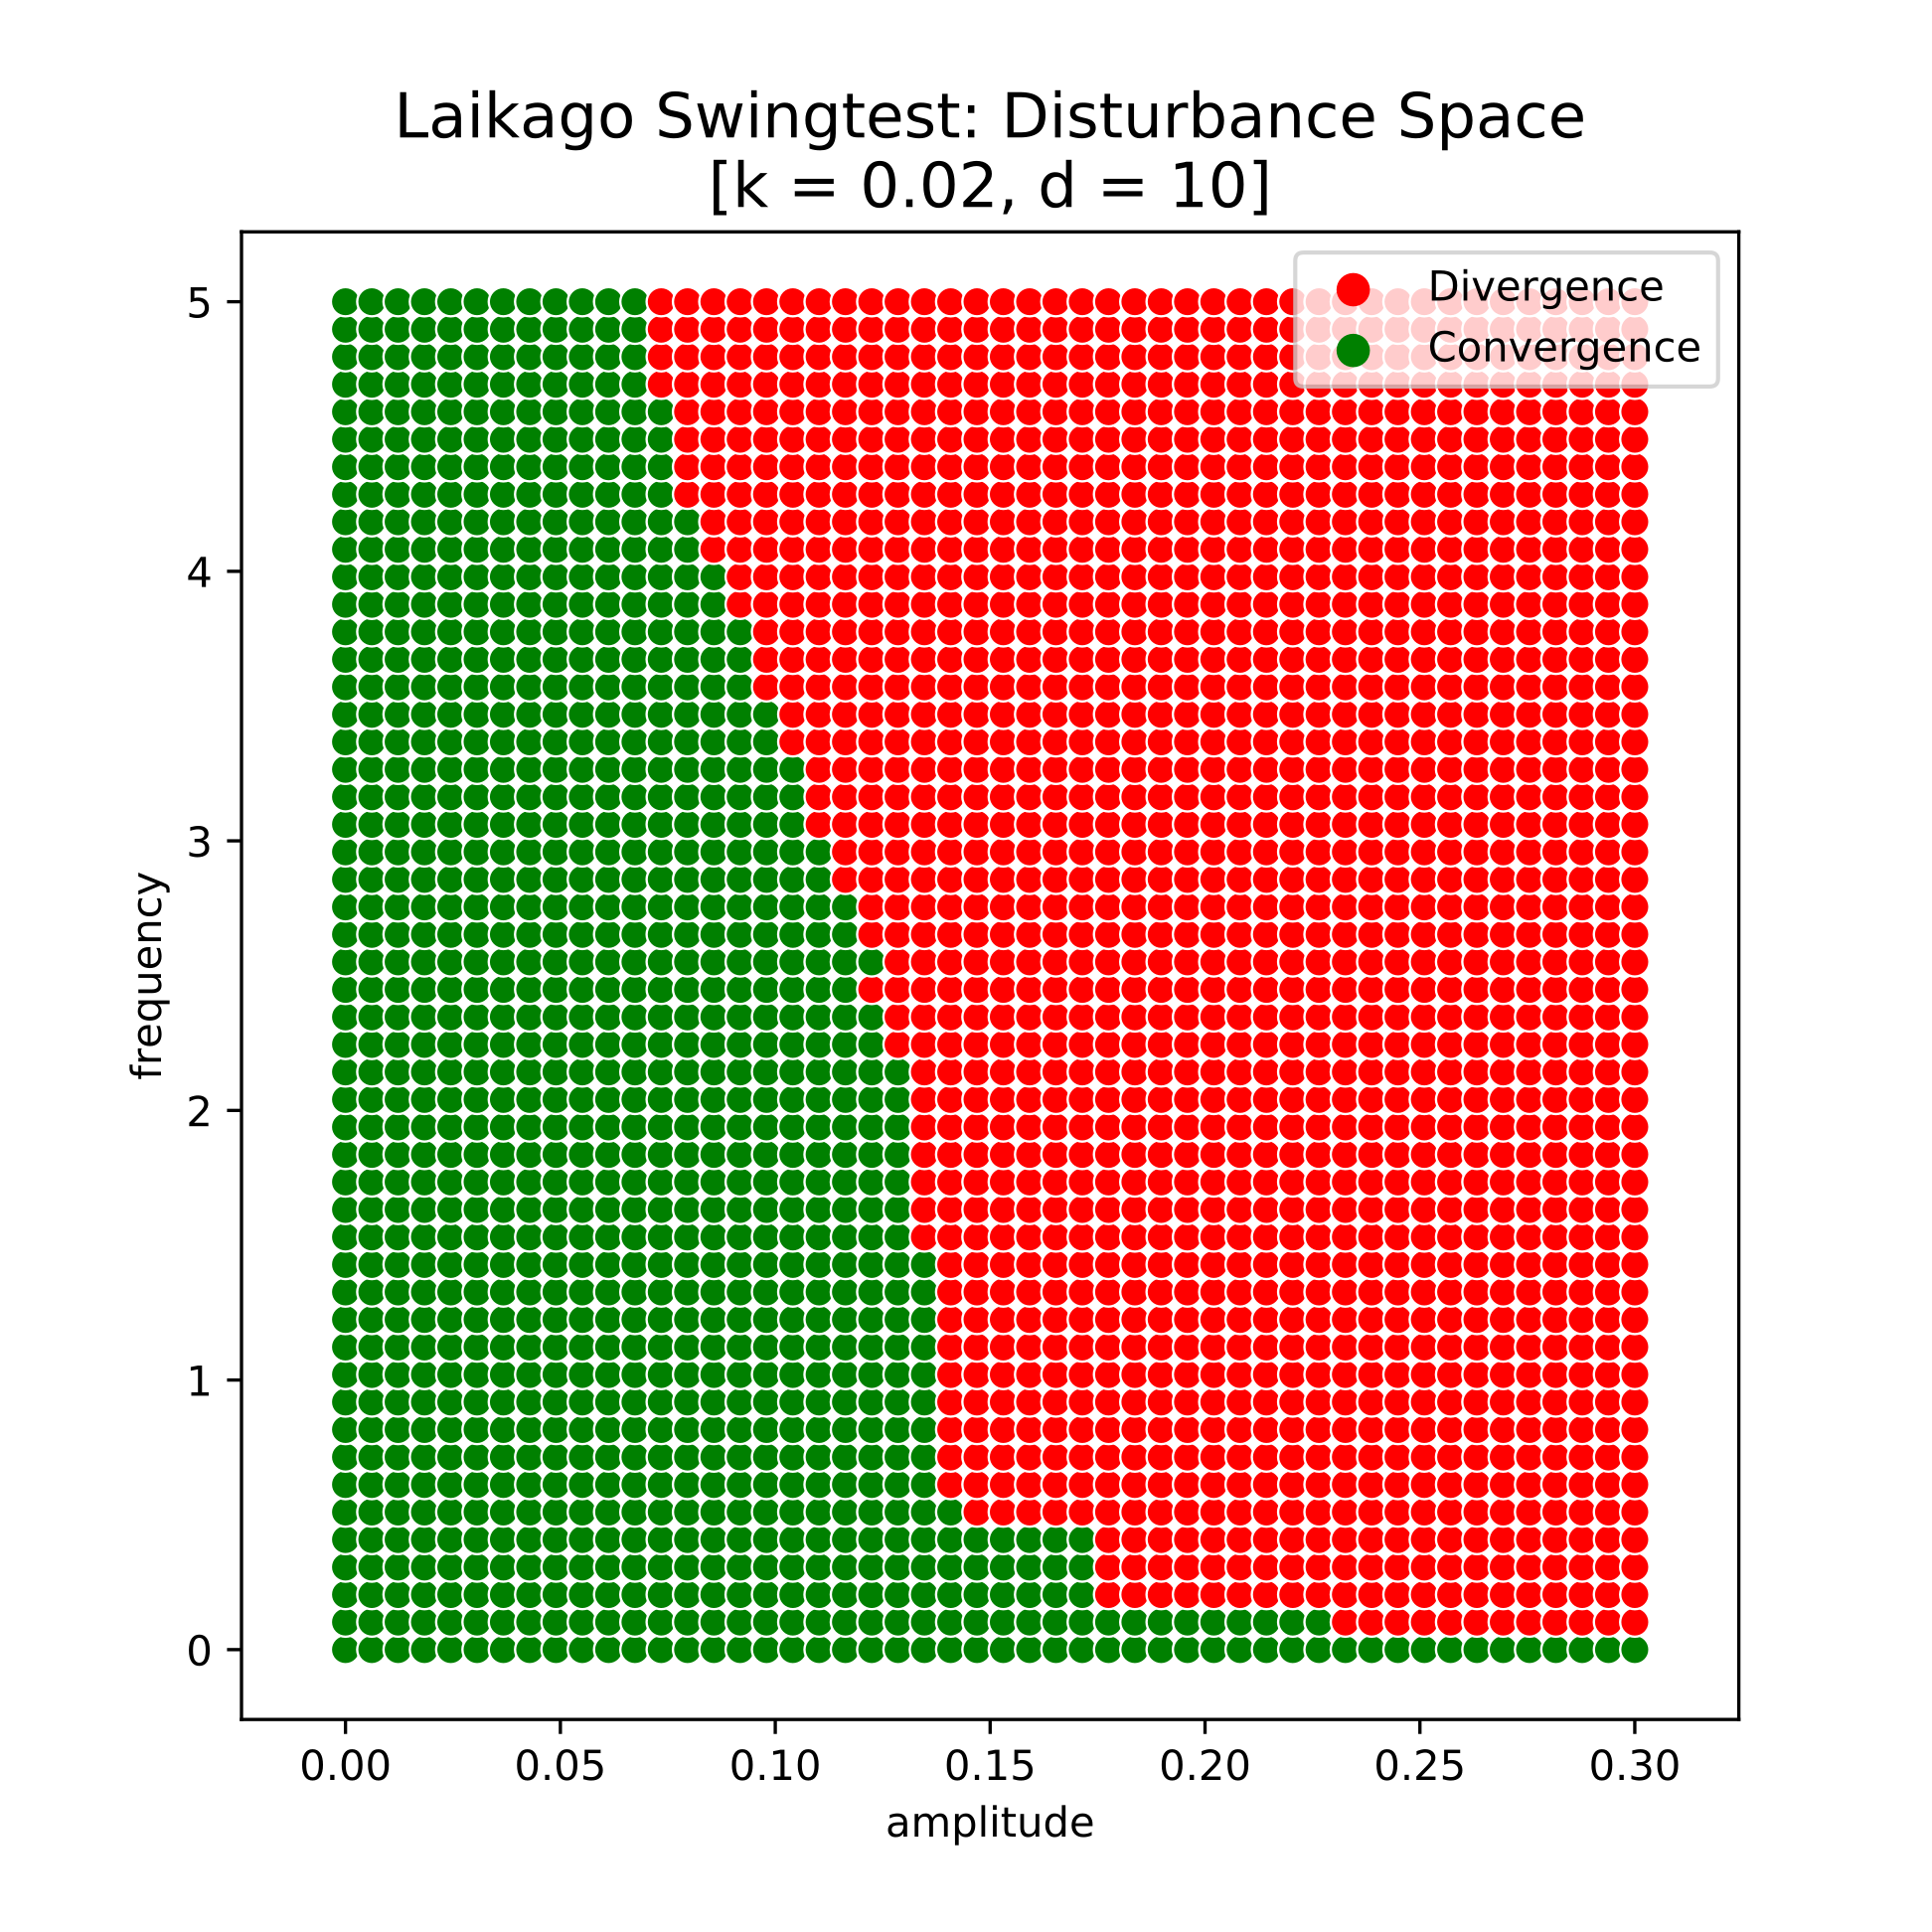
\includegraphics[width=\textwidth]{figures/swingtest_ds_bad.png} % first figure itself
            %\caption{first figure}
        \end{minipage}\hfill
        \begin{minipage}{0.33\textwidth}
            \centering
            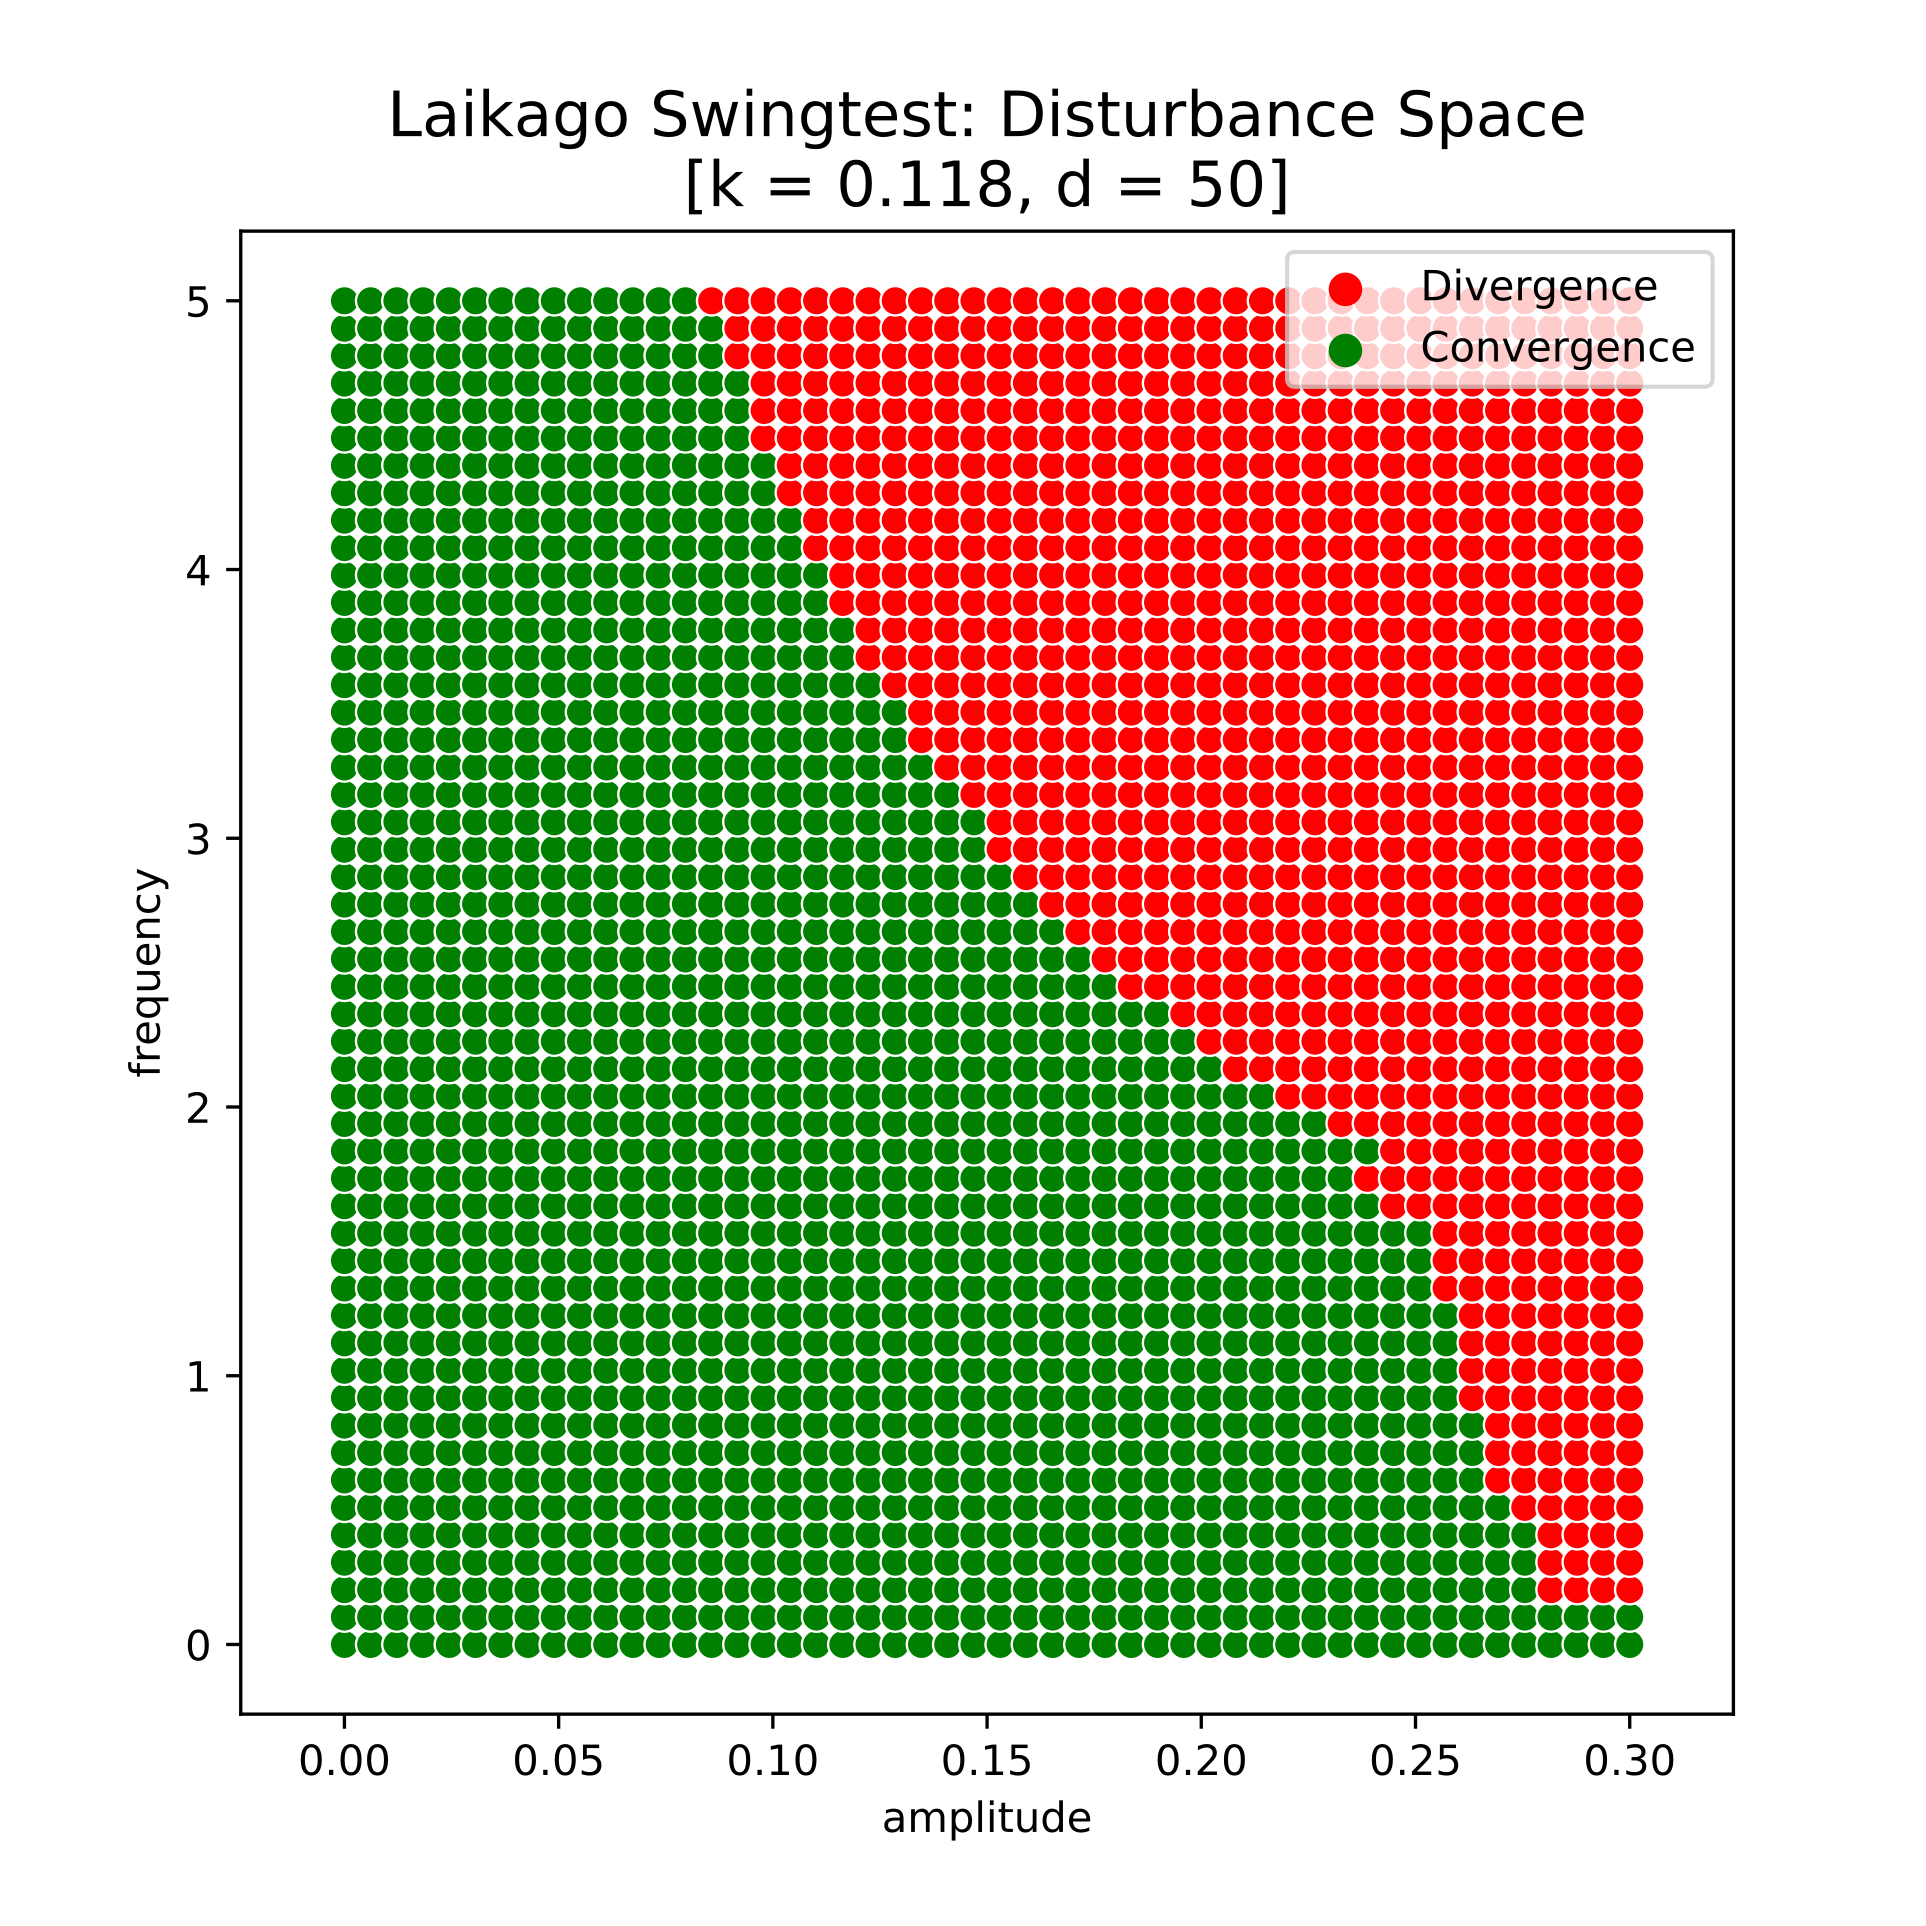
\includegraphics[width=\textwidth]{figures/swingtest_ds_medium.png} % second figure itself
            %\caption{second figure}
        \end{minipage}
        \begin{minipage}{0.33\textwidth}
            \centering
            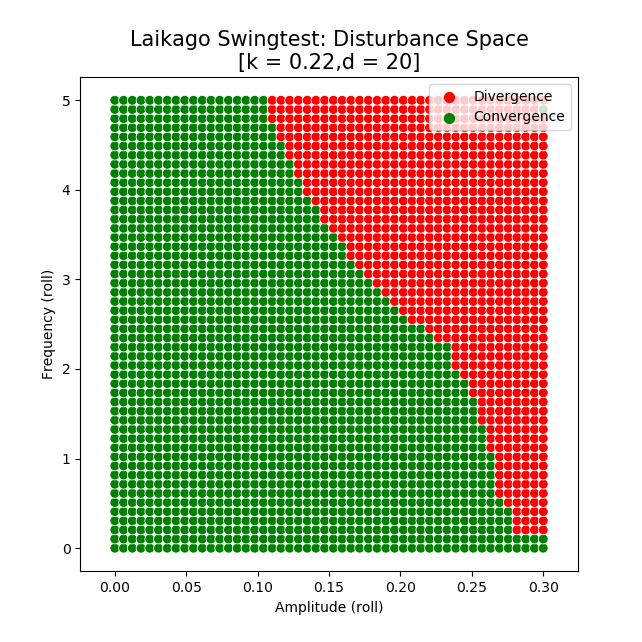
\includegraphics[width=\textwidth]{figures/swingtest_ds_opt_vfinal.png} % second figure itself
            %\caption{second figure}
        \end{minipage}

    \caption[Disturbance Spaces for Selected Parameter Sets, Drop Test]{Disturbance Spaces for specific parameter samples k and d with increasing robustness measure from left to right. A corresponding increase of the green area representing converging trajectories can be observed.}
    \label{fig:swingds}
    \end{figure}

    The results of the discretized parameter space were again further analyzed by taking three parameter samples and inspecting their disturbance spaces. There is a clear correlation between the robustness measure and size of the set of convergence, which can be seen in figure \ref{fig:swingds}. 
    \begin{figure}[h]
        \centering
        \begin{minipage}{0.5\textwidth}
            \centering
            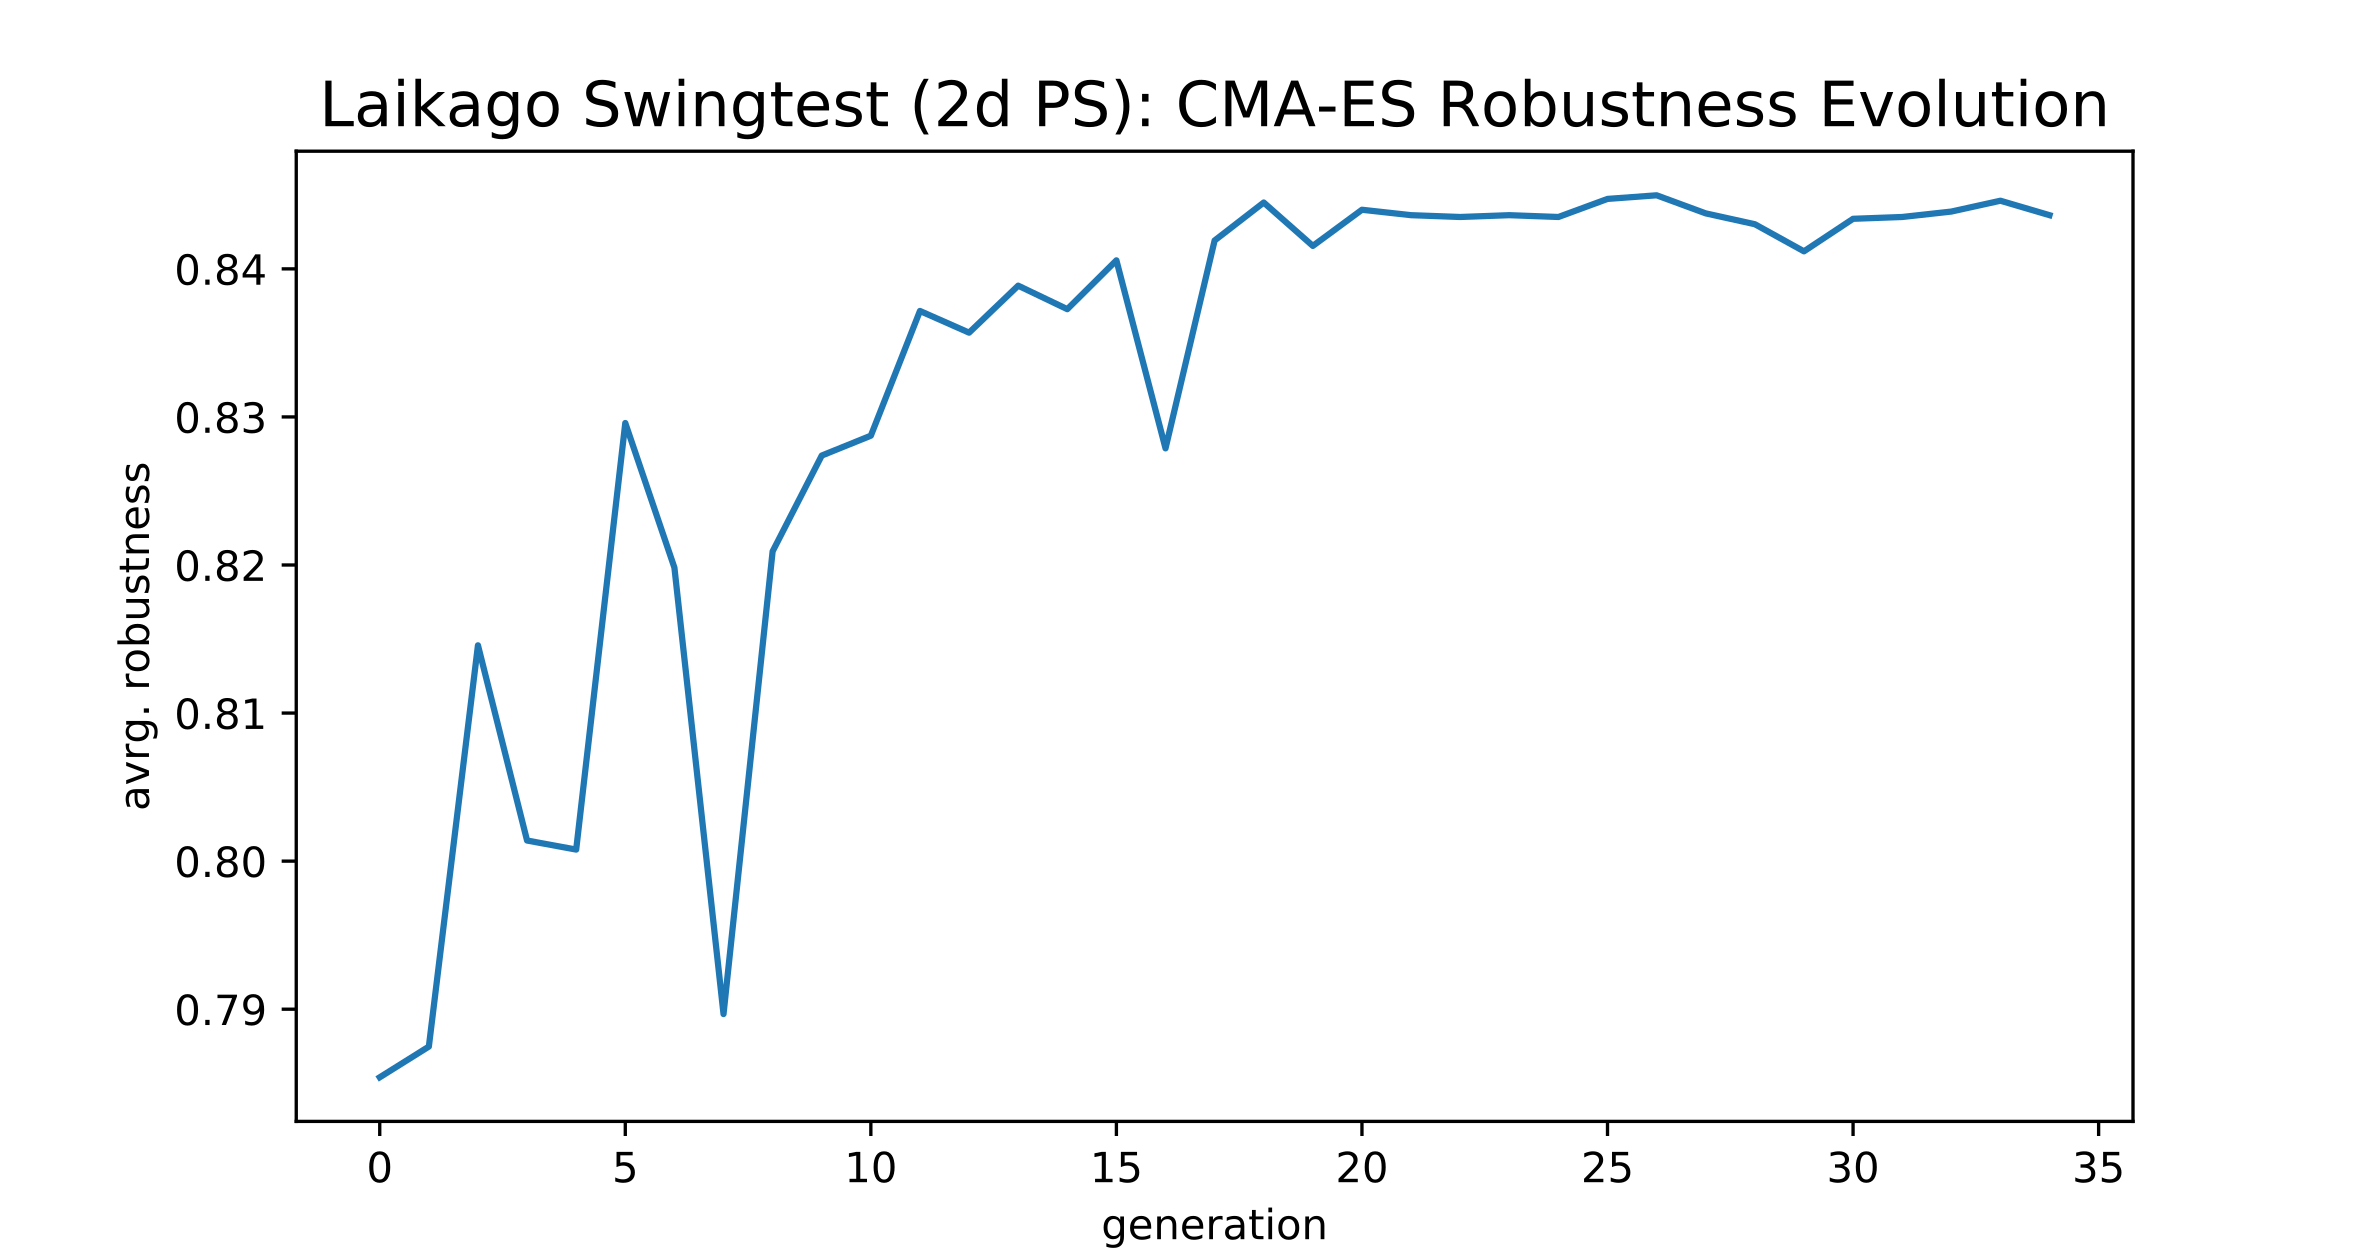
\includegraphics[width=\textwidth]{figures/swingtest_2dPS_cmaes.png} % first figure itself
            %\caption{first figure}
        \end{minipage}\hfill
        \begin{minipage}{0.5\textwidth}
            \centering
            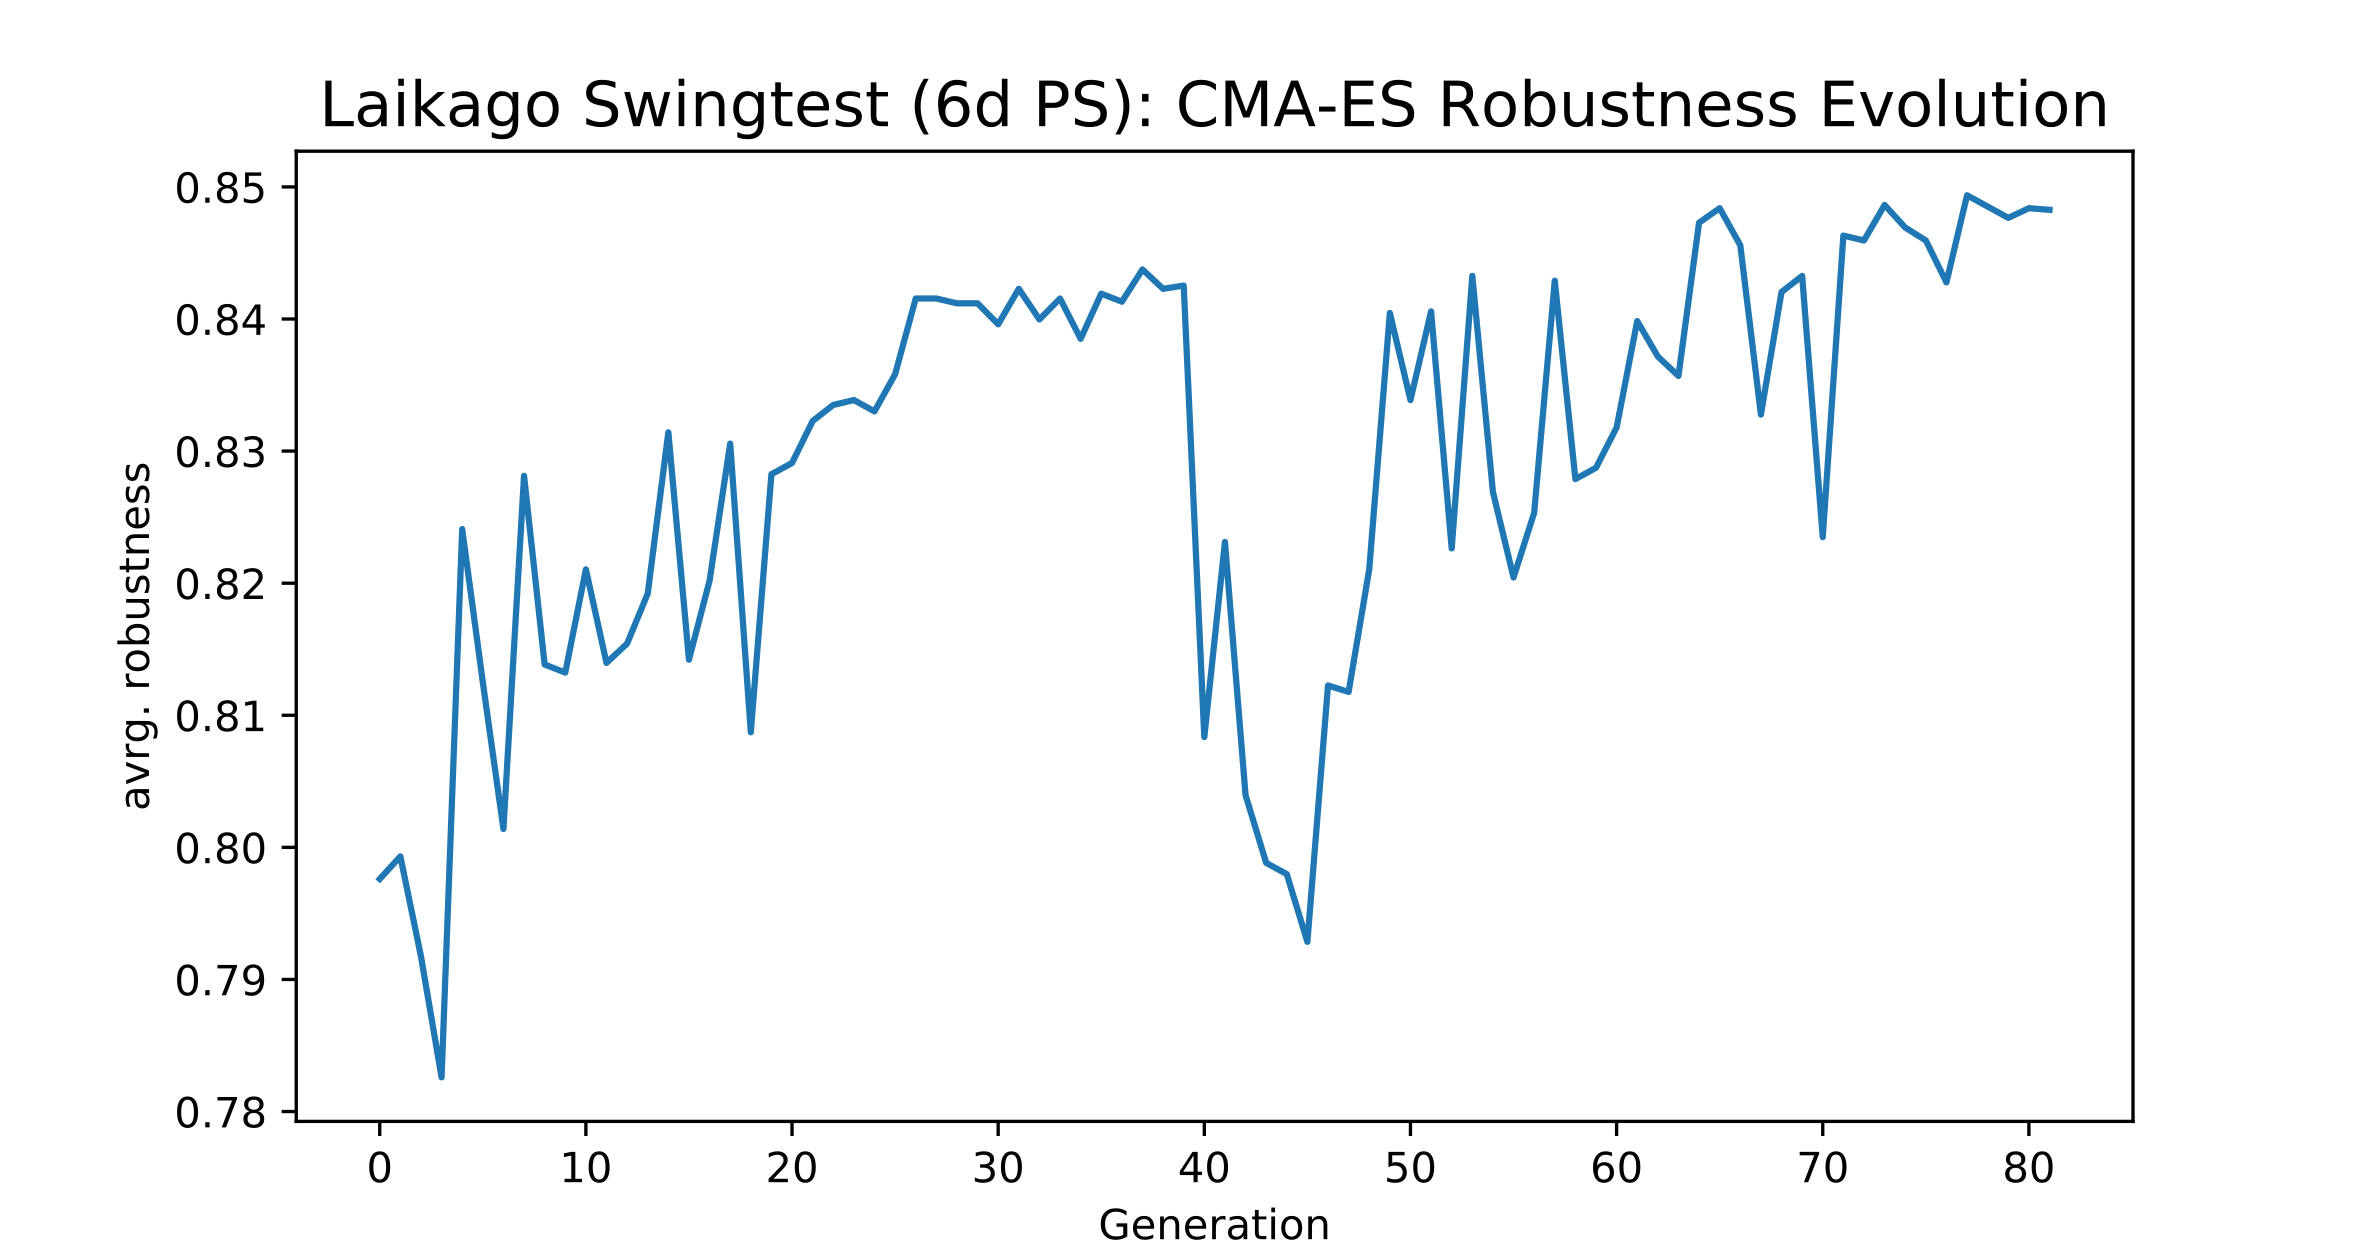
\includegraphics[width=\textwidth]{figures/swingtest_6d_cmaes.png} % second figure itself
            %\caption{second figure}
        \end{minipage}
    \caption[CMAES Evolution for 2d and 6d Parameter Spaces]{Average robustness measure for each generation of the CMAES algorithm. In the left figure stiffness and damping parameters that are equal for all motors are optimized, implying a 2d parameter space. On the right motors are grouped in three catergories, the stiffness and damping parameters of each category is taken individually in the optimization. In this 6d parameter space, slightly higher robustness measures are achieved.}
    \label{fig:cmaes}
    \end{figure}    

    The second option of optimization described in section \ref{opt} was tested here as well. Using the CMAES algorithm, comparable optimal robustness values were found, requiring less evaluations. Each "generation" of the algorithm required 4 evaluations, yielding a total of 80 revaluations before the algorithm leveled out (see figure \ref{fig:cmaes}). This corresponds to $\frac{2}{3}$ the amount of compuational effort compared to the exploration of the discretized space. 
    Here another attempt was made to increase robustness by grouping the three types of leg motors together and varying their paramters separately. This implies a 6 dimensional disturbance space $\mathsf{D}$, which would have needed $11^6=1771561$ evaluations when optimizing within the discretized space with equivalent resolution. The robustness acquired using the CMAES algorithm was marginally higher than in the 2d case, but only required approximately 280 evaluations.  






















%LEGACY


%The good thing of the conservative measure of the minimal Radius is has next to no requirements onto the shape of the attracting set of disturbances and can easily be implemented in different spaces. 

    %REF is not quite as general, as only the effects of isolated disturbances were taken into account. 

    %TRANSITION TO NEXT CHAPT

    %we ultimately want to optimize over robustness measure, so we need to look into that. 




    %The effects of disturbances on the system state can be split into three categories following nonlinear dynamical considerations:

    %1. The disturbed state still lies on the attractor. Here convergence is given immediately and the system will continue to behave as expected.

    %2. The disturbed state lies in the basin of attraction as defined in (\ref). In this case we know that the trajectory will converge and recover at some point in the future. If the BoA is not precisely know as is usually the case, this needs to be verified for every disturbance.

    %3. The disturbed state lies outsite the basin. Here the trajectory diverges and the system will not recover. As before, this needs to be checked generally. 

    %Again, for all these cases if further disturbances occur, the trajectory and therefore convergence needs to be reevaluated. 
    %Categories 1 and 2 describe desirable behaviour and 3 we want to avoid. 

    
    



    



    %In ref they used a method independent of the disturbances. 
     %NO matter what happens at any particular instace, convergence of the state trajectory long term denotes that the system will succeed in behaving as desired. 
     %These state changes bcause of disturbances  following nonlinear dynamical considerations:

    %either the new state is still part of the attractor 
    %If we start the system with an initial state that is an element of the attractor, we expect it to directly fall into the desired behaviour in form of a trajectory on the attractor.

    %or it is in the basin of attraction. As long as no further disturbances are applied, which is not very realistic for real world applications, we can immediately deduce convergence, else the further evolution of the trajectory 

    %Given a target behaviour of a system, such as holding of a pose or some periodic motion, the system fulfills that target if the state trajectory stays at the attractor long term. 

    %External disturbances acting on the system will inevitably change it's state in some way, disrupting the smooth trajectory in the phase space.  may change the system enough, convergence of a state trajectory can be interpreted as a successfull recovery from a disturbance. 
    %Looking at a set of disturbances, a larger portion of recoveries means a larger robustness within that set. This can be taken as a scalar measure of robustness within that set. If one could define a set of all possible disturbances, one could theoretically compute general robustness. At this point already one might notice that the set of disturbances may lie in a continuous space, making 

    %Here we want to do a nice drawing of initial conditions 

    %Choosing instantaneous external forces as disturbances, their effect on the system can be captured by a change on the systems state. Forces are directly related to the generalized accelerations $\ddot{\mathbf{q}}$ following Newton's second law, which in turn changes $\mathbf{q}$ and $\dot{\mathbf{q}}$ via the underlying differential equations. This implies that the set of disturbances in this case coincides with the elements of the phase space.
    %This is precisely the approch chosen for sampling of disturbances and measurement of robustness in (reference paper). A nice implications of this is that the set of disturbances from which the system recovers from coincides with the basin of attraction (defined previously). There exists literature analyzing . 
    %Also the scaling issue between q and qdot, maybe just reference it and go into detail later. 


    %However it also assumes that the system experiences a disturbance at exacltly one point and not after. This is of course quite limiting. Effects like resonance for example cannot be captured
    %Also all disturbances are treated equally. Good for generality, but one has no real control over the process (i.e. be robust to THAT thing in particular)
    %HOOWEVER


    %The disturbances are implied via the sampling of initial conditions in the phase space. Taking instantaneous External forces that act on a system will have via the underlying differntial equations a direct effect on the generalized positions and velocities $\mathbf{q}$ and $\dot{\mathbf{q}}$

    

    %Say we have a particular behaviour of our system that we want it to follow and we can define precisely. 

    %...
    %We will have a single or a set of states of our system that we have as a goal (= attractor). In the context of a quadruped this might be an upright standing position (fixed point) or a periodic walking gait. If the system is perturbed, it's state will inevitably be changed such that it is most likely not part of the attractor anymore. Finding the trajectory shows how the system will further evolve. Now convergence means that under the disturbance applied, in the long term, we will still return to and stay on the attroctor, or the system recovered, it is successful in compensating the disturbance. Divergence means something else happened, which we will just interpret as failure. So if the trajectory related to an initial condition caused by a particular disturbance converges to the attractor, the system is in a sense robust to that disturbance. 

    %If one wants to maximize robustness, really one wants to change the system or rather its parameters in such a manner that the set of disturbances which result in convergence of the state trajectory is maximized. This is the basic formulation. 

    %As detailed in REF and REF, evaluating the exact size of the set of convergiing disturbed systems, is often hard and sometimes misleading, which is why the more conservative measure of the minimal radius found with the help of random sampling is adopted (phrasing). This is in addition to the fact, that with the numerical solver at hand (ref section below), solving long trajectories and evaluating their convergence via a given attractor is much simpler to implement than the cell mapping methods detailed in previous work. 

    %This basic idea was proposed and implemented in REF, with a more focused choice of disturbance space. Disturbances themselves were disregarded and only their effects in the phase space taken into consideration. So here the goal was to maximize the set of converging inital conditions independent of their cause. However as the sampled inital conditions are just effects of disturbances, in the test we sampled and applied general disturbances, which can be thought of as subsets of the full phase space. Especially as we work with high dof systems, sampling disturbances in the full state space becomes infeasible very quickly. A generalization to disturbances as opposed to initial conditions allows us to explore more easily understandable examples where physical intuition can be applied. 


    %When referring to a system being robust to a disturbance, it means that it's trajectory in the phase space will return to the specified attractor under the influence of that particular disturbance. 

    %The size of this set can be interpreted as a measure of robustness, which was done in (REF) and is further described in.

    
    %The basic idea of robustness 

    %First explain the concept of the REF robustness measure, not how they actually compute it. 
    %Then expand to general disturbance spaces with a pointer to the meaning of DS = phase space

    
    %The goal aim of the robustness measure is to quantify the robustness of a system with a particular parameter constellation with respect to a set of distrubances. 
    %In REF, these disturbances were chosen to be initial conditions sampled from the phase space. They have a nice physical interpretation. However instantaneous forces are not the only kind of disturbance. Here we will apply the concept of the minimal Radius in REF described to some general disturbance space. This may concide with or be a subspace of the phase space, but it must not necessarily be the case. At the same time, evolution of the state trajectory and convergence will still be evaluated in the phase space. 
    

    %As in "REFERENCE", the basic idea is that the more disturbances the system can endure, i.e. it converges to the attractor, the more robust it is. Discretizing the DS and simply counting the total number of disturbances the system is robust to is impractiacal because of the possibly fractal nature of the boundary of the basin of attraction (ref) and the fact that the number of evaluations is $O((1/h)^d)$, meaning that higher resolution and a larger DS will drastically increase computational time. To remedy this issue, the in "REF" proposed minimal Radius is found which denotes the radius of the largest hypersphere that sill fits completely within the basin of attraction.

    
\chapter{Conclusion and Outlook}


physical explanation why there can't be that much optimization for swing and droptest

Implication that the system must be dynamical in nature (i.e. it must evolve). So a rudimentary control strategy must be implemented or outside forced must be applied. Don't quite know where to put this. 


further explore effects of combining disturbences of differnent sorts and the effects of the choice of bounds.

applying to systems of high dof with full phase space. Is it even possible? How much can the code be optimized?

apply to physical dimensions of systems (intuitively more drastic effects)

using the phase space as the disturbance space but heavily restricting it (actuator limits, improbable constellations etc)

Optimizing with limit cycles as attractors. 

solver (or rather finding the trajectories in general) will always be the largest bottleneck and finding methods to reduce number of trajectories to be evaluated or the computational time per trajectory would be very benefitial


Seems unlikely that this will ever be plug and play. Lots of tuning, lots of fiddling around. But there could definitely be applications, especially in novel systems where rigorous analysis is lacking. 

High complexity is still an issue. 


% ---- END MAIN PART ----


%\appendix
%\clearpage
%\renewcommand*{\chapterpagestyle}{myappendixpagestyle}

%\chapter{Information For The Few (Appendix)}

dot = f(q,qdot)
    qddot = g(q,qdot)

    order reduction:

    x = [q,qdot] => xdot = [qdot, qddot] = F(x) = [f(x), g(x)]


    q,qdot,qddot 

\section{Foo Bar Baz}


\section{Barontes}



\section{A Long Table with Booktabs}


{\scriptsize
\begin{longtable}{clccccccc}
\caption[Wordlist]{A sample list of words.}\\
\toprule
ID & Word & Word Length & WD & ETL & PTL &  WDplus \\
\midrule
\endfirsthead
\caption[]{(Continued)}\\
\toprule
ID & Word & Word Length & WD & ETL & PTL &  WDplus \\
\midrule
\endhead
\midrule
\multicolumn{9}{c}{continued on next page}\\
\bottomrule
\endfoot
%\bottomrule
\endlastfoot
\hline
1 & Eis & 3 & 4 & 0.42 & 1.83 & 0.19 \\ \hline
2 & Mai & 3 & 5 & 0.49 & 1.92 & 0.19 \\ \hline
3 & Art & 3 & 5 & 0.27 & 1.67 & 0.14 \\ \hline
4 & Uhr & 3 & 5 & 0.57 & 1.87 & 0.36 \\ \hline
5 & Rat & 3 & 5 & 0.36 & 1.71 & 0.14 \\ \hline
6 & weit & 4 & 6 & 0.21 & 1.65 & 0.25 \\ \hline
7 & eins & 4 & 6 & 0.38 & 1.79 & 0.26 \\ \hline
8 & Wort & 4 & 6 & 0.30 & 1.62 & 0.20 \\ \hline
9 & Wolf & 4 & 6 & 0.18 & 1.54 & 0.19 \\ \hline
10 & Wald & 4 & 6 & 0.31 & 1.63 & 0.19 \\ \hline
11 & Amt & 3 & 6 & 0.30 & 1.67 & 0.14 \\ \hline
12 & Wahl & 4 & 7 & 0.36 & 1.77 & 0.42 \\ \hline
13 & Volk & 4 & 7 & 0.45 & 1.81 & 0.20 \\ \hline
14 & Ziel & 4 & 7 & 0.48 & 1.78 & 0.42 \\ \hline
15 & vier & 4 & 7 & 0.38 & 1.81 & 0.42 \\ \hline
16 & Kreis & 5 & 7 & 0.26 & 1.62 & 0.33 \\ \hline
17 & Preis & 5 & 7 & 0.28 & 1.51 & 0.33 \\ \hline
18 & Re-de & 4 & 7 & 0.22 & 1.56 & 0.33 \\ \hline
19 & Saal & 4 & 7 & 0.75 & 2.10 & 0.43 \\ \hline
20 & voll & 4 & 7 & 0.48 & 1.82 & 0.24 \\ \hline
21 & weiss & 5 & 7 & 0.21 & 1.59 & 0.36 \\ \hline
22 & �r-ger & 5 & 7 & 1.16 & 2.69 & 0.59 \\ \hline
23 & bald & 4 & 7 & 0.18 & 1.56 & 0.19 \\ \hline
24 & hier & 4 & 7 & 0.40 & 1.70 & 0.43 \\ \hline
25 & neun & 4 & 7 & 0.17 & 1.52 & 0.26 \\ \hline
26 & sehr & 4 & 7 & 0.36 & 1.85 & 0.43 \\ \hline
27 & Jahr & 4 & 7 & 0.50 & 1.82 & 0.43 \\ \hline
28 & Gold & 4 & 7 & 0.04 & 1.35 & 0.20 \\ \hline
29 & T�-ter & 5 & 8 & 0.15 & 1.39 & 0.59 \\ \hline
30 & Tei-le & 5 & 8 & 0.30 & 1.71 & 0.46 \\ \hline
31 & Na-tur & 5 & 8 & 0.18 & 1.59 & 0.41 \\ \hline
32 & Feu-er & 5 & 8 & 0.30 & 1.71 & 0.45 \\ \hline
33 & Rol-le & 5 & 8 & 0.15 & 1.46 & 0.45 \\ \hline
34 & Rock & 4 & 8 & 0.29 & 1.68 & 0.25 \\ \hline
35 & Spass & 5 & 8 & 0.28 & 1.64 & 0.32 \\ \hline
36 & G�s-te & 5 & 8 & 0.49 & 1.75 & 0.66 \\ \hline
37 & En-de & 4 & 8 & 0.36 & 1.72 & 0.33 \\ \hline
38 & Kunst & 5 & 8 & 0.26 & 1.59 & 0.35 \\ \hline
39 & Li-nie & 5 & 8 & 0.45 & 1.88 & 0.63 \\ \hline
40 & B�u-me & 5 & 8 & 0.48 & 1.92 & 0.45 \\ \hline
41 & B�h-ne & 5 & 9 & 0.94 & 2.48 & 0.62 \\ \hline
42 & Bahn & 4 & 9 & 0.21 & 1.62 & 0.42 \\ \hline
43 & B�r-ger & 6 & 9 & 0.38 & 1.70 & 0.65 \\ \hline
44 & Druck & 5 & 9 & 0.60 & 2.03 & 0.31 \\ \hline
45 & zehn & 4 & 9 & 0.41 & 1.84 & 0.42 \\ \hline
46 & Va-ter & 5 & 9 & 0.36 & 1.78 & 0.40 \\ \hline
47 & Angst & 5 & 9 & 0.29 & 1.56 & 0.35 \\ \hline
48 & lei-der & 6 & 9 & 0.13 & 1.47 & 0.52 \\ \hline
49 & h�u-fig & 6 & 9 & 0.82 & 2.31 & 0.52 \\ \hline
50 & le-ben & 5 & 9 & 0.38 & 1.85 & 0.40 \\ \hline
51 & aus-ser & 6 & 9 & 1.20 & 2.26 & 0.57 \\ \hline
52 & be-vor & 5 & 9 & 1.28 & 2.75 & 0.39 \\ \hline
53 & Kai-ser & 6 & 9 & 0.92 & 2.37 & 0.53 \\ \hline
54 & Markt & 5 & 9 & 0.23 & 1.58 & 0.28 \\ \hline
55 & Os-ten & 5 & 9 & 0.21 & 1.54 & 0.48 \\ \hline
56 & Krieg & 5 & 9 & 0.33 & 1.67 & 0.50 \\ \hline
57 & Mann & 4 & 9 & 0.31 & 1.47 & 0.25 \\ \hline
58 & Hal-le & 5 & 9 & 0.24 & 1.65 & 0.45 \\ \hline
59 & heu-te & 5 & 9 & 0.44 & 1.87 & 0.46 \\ \hline
60 & in-nen & 5 & 10 & 0.36 & 1.80 & 0.45 \\ \hline
61 & Na-men & 5 & 10 & 0.28 & 1.72 & 0.41 \\ \hline
62 & jetzt & 5 & 10 & 0.70 & 2.07 & 0.32 \\ \hline
63 & kei-ner & 6 & 10 & 0.28 & 1.62 & 0.53 \\ \hline
64 & Schu-le & 6 & 10 & 1.02 & 2.12 & 0.48 \\ \hline
65 & Ar-beit & 6 & 10 & 0.34 & 1.70 & 0.52 \\ \hline
66 & An-teil & 6 & 10 & 0.27 & 1.63 & 0.53 \\ \hline
67 & di-rekt & 6 & 10 & 0.67 & 2.04 & 0.47 \\ \hline
68 & vor-her & 6 & 10 & 0.78 & 2.25 & 0.47 \\ \hline
69 & wol-len & 6 & 10 & 0.44 & 1.85 & 0.51 \\ \hline
70 & Kampf & 5 & 10 & 0.70 & 1.96 & 0.27 \\ \hline
71 & �n-dern & 6 & 10 & 1.18 & 2.62 & 0.65 \\ \hline
72 & lau-fen & 6 & 10 & 0.21 & 1.64 & 0.52 \\ \hline
73 & Eu-ro-pa & 6 & 10 & 0.23 & 1.53 & 0.66 \\ \hline
74 & statt & 5 & 10 & 1.61 & 2.86 & 0.39 \\ \hline
75 & Wes-ten & 6 & 10 & 0.29 & 1.60 & 0.54 \\
\bottomrule
\label{tab:wordlist}
\end{longtable}
}

%\clearpage
%\renewcommand*{\chapterpagestyle}{empty}

%\nocite{*}
\cleardoublepage
\phantomsection
\addcontentsline{toc}{chapter}{Bibliography}
\bibliography{references}

\end{document}
